%\documentclass[conference]{InputFiles/IEEEtran}
%\documentclass[10pt, journal]{InputFiles/IEEEtran}
%\documentclass{InputFiles/vldb}

\documentclass[sigconf, anonymous = true, screen = true, 10pt]{acmart}

%\documentclass[sigconf,10pt]{acmart} 

\settopmatter{printacmref=false} % Removes citation information below abstract
\renewcommand\footnotetextcopyrightpermission[1]{} % removes footnote with conference information in first column
\pagestyle{plain} % removes running headers
%\documentclass{InputFiles/sig-alternate-05-2015}
% % % % % % % % % % package starts...% % % % % % % % % % % % % % % % % % % % %
    \usepackage{indentfirst}
	\usepackage{graphicx} 
	\usepackage{balance}
	\usepackage{amssymb, amsmath}
%	\usepackage[thmmarks, amsmath, thref, amsthm]{ntheorem}%
%	\usepackage{amsfonts}
%	\let\proof\relax
%	\let\endproof\relax
	\usepackage{amsthm}
%	\renewcommand{\proofname}{\bf Proof}
	
	\usepackage{multirow, rotating, wasysym, url}
	\usepackage[tight]{subfigure}
	%\usepackage[retainorgcmds]{InputFiles/IEEEtrantools}
	\usepackage[ruled,linesnumbered,vlined]{algorithm2e}
	\usepackage{hyperref} %reference hyper links.
	\usepackage{color}
	\usepackage{soul}
	\usepackage{bbm}
%	\usepackage{caption2}
	\usepackage[margin=0.05in]{caption}
	\usepackage{enumerate}
	\usepackage{framed}
	\usepackage{lipsum}
	\usepackage[normalem]{ulem}
%	\captionsetup{size=footnotesize,
		%justification=centering, %% not needed
%		skip=5pt, position = bottom}
% % % % % % % % % % package ends...% % % % % % % % % % % % % % % % % % % % % %
\makeatletter
 \let\@copyrightspace\relax
\makeatother


\graphicspath{{./DrawingFigures/},{./EvaluateFigures/}, {./GraphPPT/}} 

% % % % % % % % % % New command starts...% % % % % % % % % % % % % % % % % % %
	\newcommand{\presec}{\vspace{-0.06in}}
	\newcommand{\postsec}{\vspace{-0.06in}}
	
	\newcommand{\presub}{\vspace{-0.06in}}
	\newcommand{\postsub}{\vspace{-0.06in}}
	\newcommand{\vvv}{\vspace{-0.03in}}
	\newcommand{\uuu}{\vspace{0.02in}}
	
	\newcommand{\pretablecaption}{\vspace{-0.0in}}
	\newcommand{\posttablecaption}{\vspace{-0.0in}}
	
	\newcommand{\prefig}{\vspace{-0.0in}}
	\newcommand{\postfig}{\vspace{-0.0in}}
	
	\newcommand{\prefigcaption}{\vspace{-0.0in}}
	\newcommand{\postfigcaption}{\vspace{-0.0in}}
	
	\newcommand{\adjustfigs}{\vspace{-0.0in}}
	\graphicspath{{./EvaluateFigures/}, {./GraphPPT/}, {./DrawingFigures/}}
	
%%%%%%%%%%%%%%%%%%%%%%%%%%%%%%%%%%%%%%%%%%%%%%%%%%%%%%%%%
%Only for Appendix
	\newcommand{\presecapp}{\vspace{-0.00in}}
	\newcommand{\postsecapp}{\vspace{-0.00in}}
	    
	\newcommand{\prefigapp}{\vspace{-0.0in}}
	\newcommand{\postfigapp}{\vspace{-0.0in}}
	
	\newcommand{\presubapp}{\vspace{-0.00in}}
	\newcommand{\postsubapp}{\vspace{-0.00in}}
	
	\newcommand{\prefigcaptionapp}{\vspace{-0.0in}}
	\newcommand{\postfigcaptionapp}{\vspace{-0.0in}}
%%%%%%%%%%%%%%%%%%%%%%%%%%%%%%%%%%%%%%%%%%%%%%%%%%%%%%%%%
	\newcommand{\ie}{\textit{i.e.}}
	\newcommand{\eg}{\textit{e.g.}}
	\newcommand{\etal}{\textit{et al.}}
	
	
	\newcommand{\subfigs}{\hspace{-0in}}
	\newcommand{\subfigsvert}{\vspace{-0in}}
	\newcommand{\preequation}{\vspace{-0in}}
	\newcommand{\postequation}{\vspace{-0in}}
	\newcommand{\pretheorem}{\vspace{-0in}}
	\newcommand{\posttheorem}{\vspace{-0in}}
	
		\mathchardef\Gamma="0100 \mathchardef\Delta="0101
\mathchardef\Theta="0102 \mathchardef\Lambda="0103
\mathchardef\Xi="0104 \mathchardef\Pi="0105
\mathchardef\Sigma="0106 \mathchardef\Upsilon="0107
\mathchardef\Phi="0108 \mathchardef\Psi="0109
\mathchardef\Omega="010A

\newcommand{\ovspace}[1]{\vspace{#1}}

\newcommand{\outline}[1]{}%{\textbf{#1}}

\newcommand{\dl}{\mbox{$\, [ \hspace*{-1.5pt} [\,$}}
\newcommand{\dr}{\mbox{$\, ] \hspace*{-1.5pt} ]\:$}}
\newcommand{\da}{\mbox{$\, A \hspace*{-6.75pt} A \,$}}
%\newcommand{\drightarrow}{\mbox{$\rightarrow \hspace*{-8pt} \rightarrow$}}

\newcommand{\BA}{\mbox{${\bm{a}}$}}
%\newcommand{\BB}{\mbox{${\bm{c}}$}}
\newcommand{\BC}{\mbox{${\bm{c}}$}}
\newcommand{\BD}{\mbox{${\bm{d}}$}}
\newcommand{\BE}{\mbox{${\bm{e}}$}}
\newcommand{\BO}{\mbox{${\bm{o}}$}}
\newcommand{\BP}{\mbox{${\bm{p}}$}}
\newcommand{\BQ}{\mbox{${\bm{q}}$}}
\newcommand{\BR}{\mbox{${\bm{r}}$}}
\newcommand{\BV}{\mbox{${\bm{v}}$}}
\newcommand{\BL}{\mbox{${\bm{l}}$}}
\newcommand{\BI}{\mbox{${\bm{i}}$}}
\newcommand{\BH}{\mbox{${\bm{h}}$}}
\newcommand{\BS}{\mbox{${\bm{s}}$}}
\newcommand{\BB}{\mbox{${\bm{k}}$}}

\newcommand{\wrapbox}[1]{\framebox{\begin{tabular}{c}#1\end{tabular}}}
\newcommand{\CodeIn}[1]{{\small\texttt{#1}}}
\newcommand{\Section}[1]{Section~\ref{sec:#1}}
\newcommand{\SFigure}[2]{Figure~\ref{fig:#1}(#2)}

%\usepackage{cite}
\usepackage{xspace}
\usepackage{url}
\usepackage{graphicx}
\usepackage{latexsym}
\usepackage{amssymb}
\usepackage{amsfonts}
%\usepackage{times}
\usepackage{psfrag}
%\usepackage{subfigure}
\usepackage{wrapfig}
\usepackage{comment}
%packages for algorithms
%\usepackage{algorithm}
%\usepackage{algorithmic}
\usepackage{alltt}
\usepackage{color}

\newtheorem{defn}{Definition}[section]
\newtheorem{exmp}{Example}[section]
\newtheorem{thrm}{Theorem}[section]
\newtheorem{prop}{Proposition}[section]
\newtheorem{lemm}{Lemma}[section]
\newtheorem{obsv}{Observation}[section]
\newtheorem{corr}{Corollary}[section]

%\addtolength{\textheight}{.23in} \addtolength{\textwidth}{.15in}
%\addtolength{\topmargin}{-.23in}
%\addtolength{\oddsidemargin}{.1in}
%\addtolength{\evensidemargin}{.1in}

\newtheorem{thm}{Theorem}
\newtheorem{dfn}{Definition}
\newtheorem{lem}{Lemma}
\newtheorem{cor}{Corollary}
%\newcommand{\ie}{\emph{i.e.}\xspace}
%\newcommand{\eg}{\emph{e.g.}\xspace}
\newcommand{\etc}{\emph{etc.}\xspace}
%\newcommand{\etal}{\frenchspacing{}\emph{et al{.}}\xspace}
%\newcommand{\etal}[1]{{\sl et al.{#1}}}

%%\newcommand{\thm}[1]{Theorem~\ref{thm:#1}}
%%\newcommand{\lem}[1]{Lemma~\ref{lemma:#1}}
%\newcommand{cor}[1]{Corollary~\ref{cor:#1}}
\newcommand{\fac}[1]{Fact~\ref{fact:#1}}
\newcommand{\Table}[1]{Table~\ref{tab:#1}}
\newcommand{\Figure}[1]{Figure~\ref{fig:#1}}

%\theoremstyle{plain}
\newtheorem{property}{Property}[section]
%\newtheorem{lemma}{Lemma}[section]
%\newtheorem{corollary}{Corollary}[section]
%\newtheorem{theorem}{Theorem}[section]

%\theoremstyle{definition}
\newtheorem{notation}{Notation}
\newtheorem{Definition}{Definition}[section]

%\theoremstyle{remark}
\newtheorem{fact}{Fact}[section]
\newtheorem{observation}{Observation}[section]
\newtheorem{insight}{Insight}[section]

%%\algorithmstyle{definition}
%\algsetup{indent=1em}
%\renewcommand{\algorithmicrequire}{\textbf{Input:  }}
%\renewcommand{\algorithmicensure}{\textbf{Output:}}
\newcommand{\factorial}{\ensuremath{\mbox{\sc Factorial}}}

\newcommand{\Comment}[1]{}

\renewcommand\floatpagefraction{0.999}
\renewcommand\topfraction{0.999}
\renewcommand\bottomfraction{0.999}
\renewcommand\textfraction{0.001}
\setcounter{totalnumber}{5}

		\newcommand{\Proc}{Proc. }
		\newcommand{\Conf}{Conf. }
		\newcommand{\Inte}{Int. }
		\newcommand{\Symp}{Symp. }
	\newcommand{\tabincell}[2]{\begin{tabular}{@{}#1@{}}#2\end{tabular}}
	
	\newcommand{\para}{\vspace{0.03in}\noindent\textbf}
	
	\newcommand{\figwidthdraw}{0.45\textwidth}
	\newcommand{\figwidtheva}{0.4\textwidth}
	
	\newcommand{\bm}[1]{\mbox{\boldmath{$#1$}}}
	
	\definecolor{lbq}{RGB}{0,166,0}
	\definecolor{reder}{RGB}{255,0,0}

	\definecolor{zyd}{RGB}{0,0,255}
	\definecolor{lar}{RGB}{0,100,255}
	\definecolor{xy}{RGB}{100,100,0}
	\definecolor{gray}{rgb}{0.6,0.6,0.6}
	\definecolor{shadecolor}{rgb}{0.92,0.92,0.92}
	\definecolor{jj}{HTML}{01A2FF}
% Define color used for revision
    \definecolor{reviewA}{HTML}{0000FF}
    \definecolor{reviewB}{HTML}{FF0000}
    \definecolor{reviewC}{HTML}{FF00FF}
	\definecolor{reviewD}{HTML}{00CC00}

	
	\newcommand{\ppp}{\noindent\textbf}
	\newcommand{\lbq}{\textcolor{lbq}}
	\newcommand{\zyd}{\textcolor{zyd}}
	\newcommand{\lar}{\textcolor{lar}}
	\newcommand{\xy}{\textcolor{xy}}
	\newcommand{\yt}{\textcolor{lbq}}
	
	\newcommand{\aname}{InterestSketch}
	%\newcommand{\ss}{Super-Spreader}
	
	\newcommand{\ii}{$\mathcal{I}$}
	\newcommand{\iii}{\mathcal{I}}
	
	
	
	\clubpenalty=10000
	\widowpenalty = 10000
% % % % % % % % % % New command ends...% % % % % % % % % % % % % % % % % % % %
% % % % % % % % % % Backup starts... % % % % % % % % % % % % % % % % % % % % %  
	%\clubpenalty=10000
	%\widowpenalty = 10000
	%\usepackage{caption2} %fo setlength
	%\setlength{\parskip}{0.1\baselineskip}
	%\setlength{\abovecaptionskip}{-1pt}
	%\vfill\eject % force going to next page
% % % % % % % % % % Backup ends... % % % % % % % % % % % % % % % % % % % % % %
%	

% DOI
%\acmDOI{10.475/123_4}

% ISBN
%\acmISBN{123-4567-24-567/08/06}

%Conference
\acmConference[SIGMOD'18]{}{June 10 - 15, 2018}{Houston, TX, USA} 
%\acmYear{1997}
%\copyrightyear{2016}

%\acmPrice{15.00}

\begin{document}

\title{Finding Interesting Items in Data Streams}

\author{
	Paper ID: 637. 14+4 pages.
	%	Yang Zhou, Peng Liu, Hao Jin, Tong Yang, Xiaoming Li \\
	%	Department of Computer Science and Technology, Peking University, China
	%	\IEEEauthorblockN{Yang Zhou, Peng Liu, Hao Jin, Tong Yang, Xiaoming Li}\\
	%	\IEEEauthorblockA{Department of Computer Science and Technology, Peking University, China}\\
}

\sloppy

	\begin{abstract}
	In high-speed data streams, a small fraction of items that have specific characteristics are often the focus, such as frequent items, heavy changes,
    %those source IP addresses with the most destination IP addresses (often known as Super-Spreaders), 
    Super-Spreaders, or persistent items. We call them interesting items.
	Most existing algorithms are designed for only one specific characteristic/interest, and use different data structures for different interests.
%	No previous work has so far considered the four characteristics above together. 
	%Another issue with existing algorithms is that, when memory space is limited, they can hardly guarantee both a high accuracy and a high speed at the same time. 
%Existing algorithms can be divided into two kinds. The first kind records all information of the stream, and thus is not memory efficient.
%The second kind manages to only record the interesting items, but it is challenging to differentiate interesting items from others.
	This paper generalizes these characteristics into one aspect, which we call finding interesting items in data streams. 
	%
	To find interesting items, we propose a generic framework, InterestSketch. 
	%
InterestSketch manages to record only interesting items.
To address the challenge of differentiating interesting items from others, we propose a key technique called Probabilistic Replacement and then Increment (PRI).
	%PRI is designed to record only interesting items with high accuracy and high speed, using limited memory space. 
	%The key idea of PRI is as follows. To insert a new item, we \textit{replace the current smallest item in the min-heap with a dynamic probability $\mathcal{P}$}. \textit{If the replacement is successful, the smallest interest (\eg, frequency) is incremented.}
%
	%Otherwise, we do not change the smallest item, but increase the probability $\mathcal{P}$.
	%
	Our theoretical proofs show that when replacement is successful, with high probability, the new item has a higher interest than the current smallest interest. 
	We conduct extensive experiments on three real datasets and one synthetic dataset, on four definitions of interesting items.
	Our experimental results show that compared with the state-of-the-art, for each definition of interest, our algorithm increases the insertion speed $2.2\sim 7.7$ times and decreases the error $74\sim 3207$ times.
	%
	All related code and datasets are open-source and available at Github anonymously \cite{opensource}.
\end{abstract}
	\maketitle
	
	%\vvv\vvv
\vvv\vvv
\presec
\section{Introduction} \postsec
\label{sec:intro}
\uuu
\subsection{Motivation} \postsub

%In the study of Big Data, data stream is often the representation form of data.
%
%Data stream contains consecutive items whose time of appearances might be zero, one or more. 
%
%However, under most circumstances, only a small section of data is cared in researches. 
%
%For instance, people are likely to cared about the items with the highest frequencies. 
%
%There is another likelihood that the most persistent items are the ones to study. For another example, in security, people want to find the items who are Super-Spreaders. 


Big data often comes in the form of high-speed data streams.
%
%A data stream is composed of a series of items, and each item could appear more than once.
%
A data stream is made of continuously arriving items, each of which appearing one or multiple times.
%
Although there are typically many items, people are often interested in a very limited number of them with some special characteristics, such as frequent items \cite{frequent,frequent2,frequentstream,countsketch}, heavy changes\cite{kary,revsketch, flowradar},  Super-Spreaders \cite{superspreader}, or persistent items \cite{persistentsketch,persisitem}.
In this paper, we call them \textit{interesting items}.

Finding interesting items is not new. For instance, the problem of finding frequent items is an old but still active topic in fields such as data bases and data mining. Finding Super-Spreaders and heavy changes are critical problems in security \cite{security}. Finding persistent items on the other hand is relatively recent. Note that interest can be defined in other ways. For example, to find the destination IP addresses with a large number of source IP addresses is fundamental in DDoS detection. 
%Another example is to find important items, namely to pick the items with high frequencies as well as high priority. 
% Steve: The previous example is not clear at all. What does priority refer to?

Finding interesting items is challenging, mainly because of the high speed of the data streams.
%
Therefore, it is often impossible to find interesting items without errors.
%
Fortunately, small and controllable errors are often acceptable in practice.
%
This is why sketches, a type of probabilistic data structure, have recently been used for such problems~\cite{asketch,opensketch,unbiasedsketch,coldfilter,gsketch,persistentsketch}.


\vvv
\presub
\subsection{Prior Art and Their Limitations} \postsub
\label{sec:intro:priorart}

Existing sketches often focus on one specific type of interest. 
%
For different interests, existing solutions use different data structures.
%
\hl{There are typically four definitions of interest, corresponding to four tasks: finding frequent items, finding heavy changes, finding Super-Spreaders, and finding persistent items.} For each of the four tasks, existing algorithms can be divided into two types. 
The first is called \texttt{record all}: recording all information of the stream. 
The second records a part of information of the stream, recording only \textbf{\textit{hot items}} or relying on sampling. 
In this paper, we call the items with high interest \textbf{\textit{hot items}} and the items with low interest \textbf{\textit{cold items}}.
\hl{Here we only introduce the prior art in finding frequent items and the rest three are provided in Appendix {\ref{sec:relatedwork}}.}

%\ppp{1) Finding Frequent Items:}
\ppp{Finding Frequent Items:}
Interest is defined as \textit{frequency}, \ie, the number of appearances of an item.
%
The task is to find items with large frequencies.
%
To find frequent items, two types of solutions exist. The first type, \texttt{record all}, records the frequencies of all items.
%{\color{jj}For this task, \texttt{record all} algorithms record  the frequencies of all items.}
Typical algorithms are made of a sketch (\eg, sketches of CM~\cite{cmsketch}, CU~\cite{cusketch}, and Count \cite{countsketch}) plus a min-heap, and ASketch~\cite{asketch}. Recording the frequencies of cold items is unnecessary. The second kind only records hot items: the information of items with large frequencies. Typical algorithms are SpaceSaving~\cite{spacesaving}, Unbiased SpaceSaving~\cite{unbiasedsketch}, Lossy Counting \cite{losscounting}, and Cold filter~\cite{coldfilter}.
%The third kind is called \texttt{hybrid} in this paper, which adds a filter to filter cold items before recording the information of items with large frequencies. The typical algorithm is called .
%
SpaceSaving and the Unbiased SpaceSaving use a min-heap-like data structure to record hot items. 
When the min-heap is full, the smallest frequency is incremented by one irrespective of the incoming item being cold or hot. However, in practice, there are many cold items that have a \textit{negative impact} on the recorded frequencies, leading to relatively poor accuracy.
%
Our algorithm belongs to the second kind, but manages to minimize this negative impact without using any additional data structure. 

%\ppp{2) Finding Heavy Changes:}
%Here, a data stream is equally divided into $n$ periods (also known as time windows or intervals). We define interest as \textit{change of frequency}, \ie, the difference of frequency of an item in two adjacent periods.
%
%Again, the first type of solution is to \texttt{record all}, including k-ary \cite{kary}, the reversible sketch \cite{revsketch}, and FlowRadar \cite{flowradar}. 
%They build one data structure to record all items in each period, and then manage to decode and report heavy changes. 
%
%The second kind manages to record only hot items, and the typical algorithm being Cold filter \cite{coldfilter}.
%Cold filter first uses a filter to filter cold items, and then focuses on hot items. We aim to achieve a higher accuracy than Cold filter without any additional data structure.


%\ppp{3) Finding Super-Spreaders:}
%Each item is a packet with a source IP address and a destination IP address. We define interest as \textit{connections}, \ie, the number of destination IP addresses for a given source IP address. The problem is to find source IP addresses with large number of connections.
%
%Again, two kinds of solutions exist. The first, \texttt{record all}, records the information of all packets. Typical algorithms are Two-dimension bitmap \cite{twodimensional} and OpenSketch \cite{opensketch}. 
%The second kind, \texttt{record samples}, samples packets before recording the information of packets. Sampling achieves memory efficiency at the cost of poor accuracy.
%The typical algorithms here are called one-level filtering \cite{superspreader} and two-level filtering \cite{superspreader}. We aim to record only Super-Spreaders without sampling, to achieve a higher accuracy. 

%\ppp{4) Finding Persistent Items:}
%Here, a data stream is equally divided into $n$ periods. 
%
%We define interest as \textit{persistency}, \ie, the number of periods in which the item appears.
%
%In each period of the stream, the persistency of an item is incremented only once or not changed. 
%
%The problem is to find items with high persistency.
%
%Again, two types of solutions exist. The first, \texttt{record all}, records the information of all packets. The typical algorithm is PIE \cite{persisitem}. The second kind, \texttt{record samples}, samples before recording the information of items. The typical algorithm is small-space \cite{smallspace}. 
%
%We aim to record only persistent items to achieve a higher accuracy. 

%In contrast, we aim to design a generic framework, which can be used for finding any interesting items with high speed and high accuracy at the same time.


 
\presub \uuu
\subsection{Our Solution} 
\postsub \uuu \uuu
%
In this paper, we propose a generic framework, named \aname, to find interesting items, such as frequent items, heavy changes, Super-Spreaders, and persistent items.
%

Now we use a simple example to explain our key idea of differentiating hot items from others. Consider the following problem: given a data stream, how to find the most frequent item with only one bucket?
%
The bucket has two fields: item ID and frequency.
%
The key operation lies in the following situation: the incoming item $e_1$ is different from \texttt{the original item} $e_0$ with frequency $f_0$ kept in the bucket. 
%
The most widely used algorithm, SpaceSaving \cite{spacesaving}, just replaces $e_0$ with $e_1$, and increments the frequency from $f_0$ to $f_0+1$.
%
In contrast, our technique is called \textit{\textbf{Probabilistic Replace then Increment (PRI)}}: replacing $e_0$ with the incoming item $e_1$ with a replacement probability $\mathcal{P}$.
%
If $e_1$ successfully replaces $e_0$, we increment $f_0$ by $\lfloor t_{fail}/f_0\rfloor $ and reset $t_{fail}$ to 0, where $t_{fail}$ is the number of replacement failures. Otherwise, we increment $t_{fail}$ by 1.
%when the number of replacement failures is small, we keep $f_0$ unchanged; if $e_1$ replaces $e_0$ when the number of replacement failures is large, \yt{we increment $f_0$ by 2;} and in other cases, we increment $f_0$ by 1.
After each unsuccessful replacement, the replacement probability $\mathcal{P}$ increases.
%
Further, to make replacement as correct as possible, \ie, given that we want only hot items to replace cold items, \textit{the value of $\mathcal{P}$ decreases as $f$ increases.}
%
More details about $\mathcal{P}$ are provided in Section \ref{sub:findinterest}.


\ppp{Analysis:} 
%lbq.. suppose
SpaceSaving supposes the incoming item is always hotter than the original item in the bucket. At the end, the item kept in the bucket must be the last incoming one and the interest is the sum of the interests of all distinct items in the data stream. 
The unbiased SpaceSaving \cite{unbiasedsketch} first increments the frequency and then tries replacement, achieving unbiased error at the cost of poor accuracy.
%
In contrast, we differentiate hot and cold items by using PRI. Compared with cold items, hot items have a higher probability of replacing the original item.
%
After each successful replacement, incrementing the frequency is reasonable.
%
%In this way, we divide the data stream into two parts: with high probability, hot items are maintained and cold items are discarded.
%
%In this way, with high probability, we keep hot items and discard cold items.





%Given a specific definition of interest, \aname{} can find interesting items quickly and accurately.

\ppp{Main Experimental Results:}
We compare our \aname{} with the state-of-the-art algorithms in each of the aforementioned four tasks.
In finding frequent items, \aname{} reduces the error $74\sim 3207$ times and improves the insertion speed $2.2\sim 7.7$ times. In finding heavy changes, \aname{} improves the precision $3.6\sim 6.2$ times when using only 1/20 of the memory size of other algorithms and improves the insertion speed $2.1\sim 3.0$ times. In finding Super-Spreaders, \aname{} reduces the error $18\sim 31$ times. In finding persistent items, \aname{} reduces the error $115\sim 50212$ times when using only 1/20 of the memory size of other algorithms and increases the insertion speed $1.4\sim 4$ times.
% Suppose that there is one bucket with record of the ID and frequency of the item. For a incoming data stream, we want to store the most frequent item in the bucket. 
% %
% We keep the Id and frequency $f$ of the first incoming item in the bucket. 
% %
% When the next item comes, in Space-Saving, the original item is replaced by the incoming item and the frequency is added by one anyway.
% %
% In contrast, we replace the original item with the new item with a probability of $1/(f+1)$. If replacing successfully, the frequency is added by one. Otherwise, the frequency remains unchanged.
% %
% In Space-Saving, the item kept in the bucket must be the last incoming one in the data stream and the frequency is the number of items in the stream. In our algorithm, the larger frequency the item has, the higher probability the item will be kept in the bucket.  


%\presub
%\vvv\vvv
%\subsection{Key Contribution} %\postsub

\ppp{Key Contributions:}

1) We propose a generic framework called InterestSketch, which can find interesting items with high accuracy and high speed using small memory.

	2) To verify the generality of our framework, we apply the framework to four specific tasks, including finding frequent items, finding heavy changes, finding Super-Spreaders, and finding persistent items.

3) We derive the error bounds and several theoretical properties of InterestSketch.
% Steve: reasonable means absolutely nothing for a proof.

	4) We conduct extensive experiments on three real datasets and one synthetic dataset. Our results show that InterestSketch significantly outperforms all existing algorithms in terms of both accuracy and speed.



% \begin{itemize}
% 	\item We propose a generic framework called InterestSketch, which can find interesting items with high accuracy and high speed using small memory.
% 	\item To verify the generality of our framework, we apply the framework to four specific tasks, including finding frequent items, finding heavy changes, finding Super-Spreaders, and finding persistent items.
% 	\item We derive the error bounds and several theoretical properties of InterestSketch.
% % Steve: reasonable means absolutely nothing for a proof.
% 	\item We conduct extensive experiments on three real datasets and one synthetic dataset. Our results show that InterestSketch significantly outperforms all existing algorithms in terms of both accuracy and speed.
% \end{itemize}


% \ppp{Roadmap:} Section \ref{sec:relatedwork} surveys the related work.
% We present our algorithms in Section \ref{sec:basicAlgorithm}.
% The algorithm is optimized in Section \ref{sec:optimization}. 
% We apply the algorithm to four tasks in Section \ref{sec:application}. 
% We derive proofs of our algorithms in Section \ref{sec:proof}.
% The experimental results are showed in Section \ref{sec:experiments}.
% The conclusion of this paper is in Section \ref{sec:conclusion}.




	
	%\presec
%\section{Background and Related Work} \postsec
%\label{sec:relatedwork}

%There are the four typical problems related to finding interesting items: 1) finding frequent items; 2) finding heavy changes; 3) finding Super-Spreaders; and 4) finding persistent items. In this section, we first state the considered problems. Then, we introduce the typical algorithms for each of them respectively.

\presec
\section{Problem Statement} \vvv
%This section show the definitions of typical tasks, and the related work briefly introduced in the Introduction is described in detail in Appendix \ref{sec:relatedwork}.

{\color{reviewA}
\ppp{Finding Interesting Items:}
\hl{A data stream $\mathcal{S}$, either limited or unlimited, consists of items, where each item can appear more than once. We can use ``interest'' to describe one property of concern. Finding interesting items means to report all the items with interests larger than a given threshold.
%
Different definitions of interest correspond to different tasks of data streams. The size of each item can vary according to the definitions. Next, we show four typical tasks.
}}

{\color{reviewA}
\ppp{Finding Frequent Items:}
\hl{In finding frequent items, the interest is defined as \textbf{frequency}, i.e., the number of appearances of each item. Finding frequent items includes two problems: heavy hitter and top-k. The difference is that heavy hitter is to find items whose frequencies are larger than a given threshold, while top-$k$ is to find top-$k$ frequent items. Since the two problems are similar, we will focus on the problem of heavy hitter.}}

\ppp{Finding Heavy Changes:}
Given a data stream, we divide it into equal-sized periods. 
In finding heavy changes, the interest is defined as \textbf{change of frequency}, \ie, the change of frequency of an item in two adjacent periods.
%Given two adjacent periods, each item has a frequency. 
The frequencies of some items could drastically change between two adjacent periods. \hl{Reporting and Analyzing such changes is important in security} \cite{flowradar,revsketch}. \hl{Finding heavy changes is to find items whose changes of frequency are larger than a given threshold.}


\hl{\noindent\textbf{Finding Super-spreaders:}
In computer networks, each item is a packet with a source IP address and a destination IP address. A specific source IP address can send packets to many destination IP addresses. Super-spreaders are those source IP addresses that have more destination IP addresses than a given threshold. When the interest is defined as \textbf{connections}, i.e., the number of destination IP addresses for a given source IP address, the problem will be finding super-spreaders. In other words, super-spreaders are the most influential individuals spreading information, because they have more connections than a given threshold. }


\noindent\hl{\textbf{Finding Persistent Items:}
Again, given a data stream, we equally divide it into equal size periods. For a specific item, its \textbf{persistency} indicates the number of periods in which the item appears. 
No matter an item appears either once or more in a period, its persistency is incremented by one because there exists this item in this period. When we define interest as persistency, the problem will be to find persistent items. In other words, we want to find the items whose persistency is more than a given threshold.
}



\noindent\textcolor{reviewA}{\textbf{Other problems:} \hl{While we focus on the above four problems, there are also some other problems with different definitions of interest.
1) Finding DDoS victims. This is similar to finding Super-Spreaders. In this problem, interest is defined as connections. This problem is to find those destination IP addresses that have more source IP addresses than a given threshold. 
2) Finding Advance Persistent Threats (APT). This problem needs to find items that are persistent but not frequent.
3) Finding both frequent and persistent items. In some application, one may need to find items that are both frequent and persistent items.} }







\begin{comment}
\ppp{Finding Super-spreaders:}
In computer networks, each item is a packet with a source IP address and a destination IP address. A specific source IP address can send packets to many destination IP addresses. When the interest is defined as \textbf{connections}, i.e., the number of destination IP addresses for a given source IP address, the problem will be about finding super-spreaders.


\ppp{Finding Persistent Items:}
Again, given a data stream, we equally divide it into equal size periods. 
%
For a specific item, its \textbf{persistency} indicates the number of periods in which the item appears. 
%
In each period, if an item appears, either once or more, its persistency is incremented by one. 
%
When we define interest as persistency, the problem will be to find persistent items.
\end{comment}
	

	\presec
\section{InterestSketch: Basics} \postsec
\label{sec:basicAlgorithm:frequent}

In this section, we first present our generic framework -- InterestSketch, and then show how to use our framework to find frequent items, heavy changes, super-spreaders, and persistent items.

%  Safe replacement...
%1. 大流成功replace概率高
%2. 不会一直不成功
%3. 进一步降低小流成功replace的概率。preparation cell
%4. 末尾淘汰制。。
%5. 开始预备cell宁愿空着。
%6. ID 太长可以用指纹代替。
%7. 用概率的方法替换可以提高大流成功替换的概率,但总有各种不同形式的不合理的替换,我们用 预备cell的方法就是为了努力消除各种不合理替换,从而提高accuracy。












%












    			\presub
\subsection{The InterestSketch Framework}
\postsub
\label{sub:findinterest}
%
\begin{figure}[htbp]
	\centering
	\prefig
	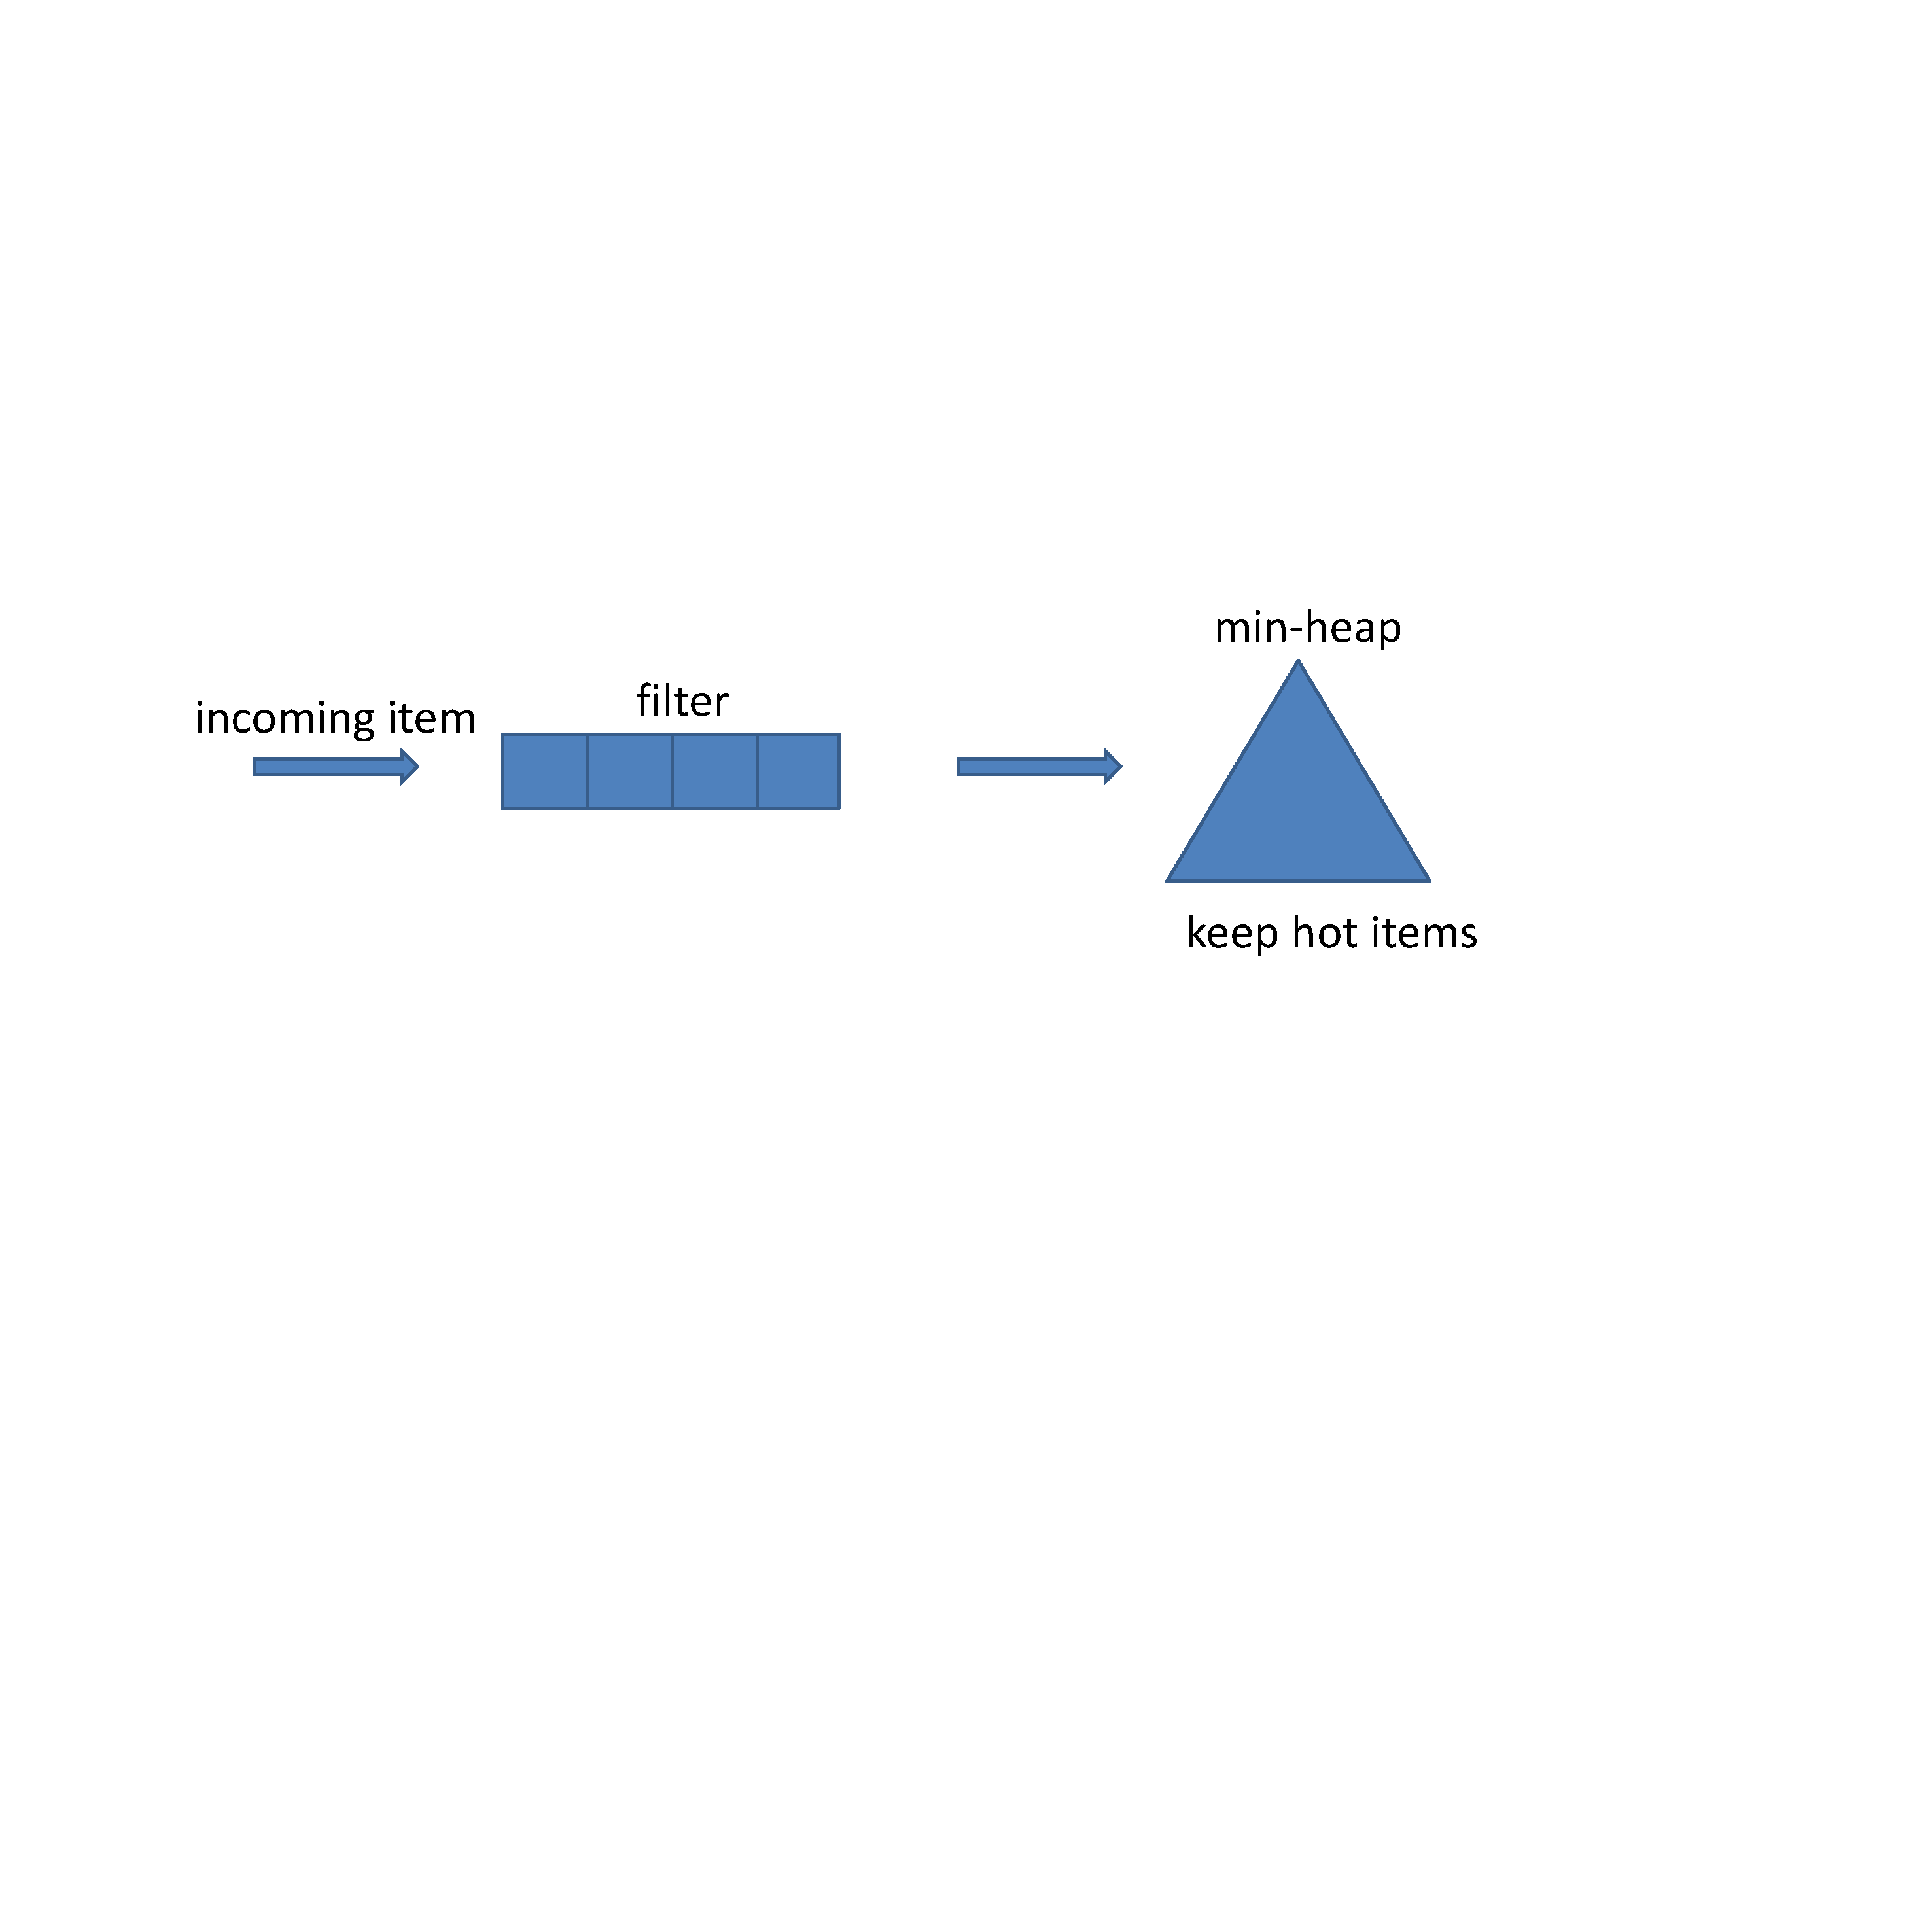
\includegraphics[width=0.45\textwidth]{framework}
	\prefigcaption \vspace{-0.05in} \vspace{-0.05in}
	\caption{The \aname{} framework.}
	\label{draw:interestframework}
	\postfig \vspace{-0.05in}
\end{figure}
%
To make our novelty clear, we first show the basic framework. It is simple: a filter (optional) and a min-heap. ``Optional'' means that some tasks do not need the filter.
%
Our key novelty is \textbf{\textit{the PRI technique}}.
%
In next Section (Section \ref{sec:optimization}), we will replace the min-heap to minimize the overhead of both time and space.

%achieve both memory efficiency and space efficiency.

\ppp{Data Structure (Figure \ref{draw:interestframework}):} 
The \aname{} framework consists of two parts. The first is a Bloom filter~\cite{BF1970}, used to remove duplicates in the incoming items. 
%
%Different definitions of interest has different operations of items in the Bloom filter. 
Duplicates removal is necessary because the interest \ii might not be incremented for every incoming item. For example, when finding persistent items, in each period, each incoming item can only increment the corresponding persistency by one, even though it might appear more than once in that period. 
%
The second part is a min-heap keeping hot items. In the min-heap, each node stores the information of an item, including item ID and interest \ii. The root node stores the item with the smallest interest. 

A Bloom filter~\cite{BF1970} is a compact data structure consisting of a number of bits and is often used when judging whether an item exists in a set or not. 
%
It is associated with $z$ hash functions.
%
There are mainly two operations for this data structure. 
%
The first is to insert an item $e$. 
%
The $z$ hash functions are first computed to pick out $z$ bits in the Bloom filter, and then all the $z$ bits are set to 1.
%
The second operation is to judge whether an item belongs to the set. The same $z$ hash functions are first computed to get the $z$ bits, and only if all the $z$ bits are 1, the Bloom filter reports true; otherwise, it reports false.
%
If the item is indeed in the set, true is always reported, \ie, it has no false negative error. 
%
In some cases, when an item does not belong to the set, the Bloom filter might also report true, which is called as false positive. However, the probability of false positive is often small enough to be acceptable in practice. 
%
Therefore, Bloom filters are used in various fields, especially in approximate data stream processing.


%%
\ppp{Insertion:}
Given an incoming item $e$, we first check the Bloom filter to judge whether $e$ is a duplicate: if the Bloom filter reports true, which means $e$ is a duplicate, and then $e$ is discarded. Otherwise, $e$ is inserted into the Bloom filter, and then we insert $e$ in the min-heap. There are two cases:

\textit{Case 1:} The item $e$ is in the min-heap. In this case, we increment the interest \ii{} by one.

\textit{Case 2:} $e$ is not in the min-heap. If the min-heap is not full, we insert $e$ into the min-heap. If the min-heap is full, we propose a technique named Probabilistic Replacement and then Increment (PRI for short) to \textit{probabilistically judge whether the incoming item is hot or cold.}

%%
\ppp{Probabilistic Replacement and then Increment (PRI):} This technique is the key novelty in this paper. Our PRI works as follows.
Suppose that the root node of the min-heap stores item $e_{min}$ with interest $\iii_{min}$.
Given an incoming item $e$ which is not in the min-heap, we replace $e_{min}$ with incoming item $e$ with a probability
%
$$\mathcal{P}=\frac{1}{2*\iii_{min}-
t_{fail}+1}$$
where $t_{fail}$ is the number of replacement failures.
%
If $e_{min}$ is successfully replaced by $e$, indicating that the interest of $e$ is likely to be larger than $e_{min}$, we increment the interest of $e_{min}$ from $\iii_{min}$ to $\iii_{min}+\lfloor t_{fail}/\iii_{min}\rfloor$ and set $t_{fail}$ to 0. 
%
Otherwise, $t_{fail}$ is incremented by 1.
%
For convenience, $\iii_{min}+\lfloor t_{fail}/\iii_{min}\rfloor$ is abbreviated to  $\iii_{min}+ t_{fail}/\iii_{min}$ in this paper.

{\color{reviewD}\hl{
\noindent\textbf{Designing the Expression of $\mathcal{P}$:}
We carefully design the expression of $\mathcal{P}$ to meet the following five properties. 
1) To successfully replace the original item, the value of $t_{fail}$ should reach an expectation of $\iii_{min}$.
%
2) The larger $\iii_{min}$ is, the less likely it is to be replaced.
3) The more replacement failures there are, the more likely the replacement will happen. 
4) When the number of replacement failures reaches $2*\iii_{min}$, the probability $\mathcal{P}$ increases to 1. This can avoid too many replacement failures.
5) When the replacement happens when number of replacement failures is small, $t_{fail}/\iii_{min}$ =0, we do not increase the smallest frequency. When the replacement happens when number of replacement failures is large, $t_{fail}/\iii_{min}$ =2, we increase the smallest frequency by 2. In other cases, we increase the smallest frequency by 0 or 1. 
}}


%
%We find that when the expression of $\mathcal{P}$ meets the above five properties, the accuracy is high and varies slightly.
%
%For example, we can use $\mathcal{P}=1/(3*\iii_{min}-t+1)$, or $i/(2*\iii)$, or.


%Analysis: In setting the probability of replacement, different probability leads to different accuracy. There are several alternatives: ({\color{red}$1/(\iii_{min}+1)$, $1/\iii_{min}$, $1/\iii_{min}^2$, $1/\lambda*\iii_{min}$, $1/2^{\iii_{min}}$, \textit{etc}.}) $1/(\iii_{min}+1)$, $1/\iii_{min}^2$, $1/(\lambda*\iii_{min})$, $1/c^{\iii_{min}}$, \textit{etc}. 
%Finally, we choose $1/(\iii_{min}+1)$ for two reasons. First, to successfully replace the original item, the number of new incoming items should reach an expectation of $\iii_{min}+1$.
%Second, the results of experiments show that the accuracy is the highest when the probability is  $1/(\iii_{min}+1)$ compared with all the other alternatives. 
%Otherwise, the interest $\iii_{min}$ remains unchanged.


%%
\ppp{Report:}
To report the items above a given threshold $\mathcal{T}$, we simply traverse the min-heap to return the items with interests larger than $\mathcal{T}$. 
%(see Algorithm \ref{alg:basic}).
\begin{comment}

Every time the interest of the item changes in the min-heap, we should adjust the min-heap. Therefore, we adjust the min-heap in lines $8^{th}$, $12^{th}$, and $18^{th}$.
%
Lines $14$ to $20$ of Algorithm \ref{alg:basic} are the implementation of the PRI technique.
%
Besides, in line $14$, we calculate the probability $\mathcal{P}$ by producing a random number between 0 and 1, because the probability that the random number is less than $\frac{1}{2*f_{min}-t_{fail}+1}$ is approximately equal to $\mathcal{P}$.
\end{comment}

\begin{comment}

\begin{algorithm}
	%	\SetLine
	\KwIn{An item $e_i$}
	$random()\in [0,1]$\\
	\eIf{$e_{i} \in$ Bloom\_filter}
	{
	    $return$\;
	}
	{
	$Bloom\_filter.insert(e_i)$\;
	\eIf{$e_{i} \in min\_heap$}
	{
		$Interest(e_{i})++$\;
		$min\_heap.adjust()$\;
	}
	  {
        \eIf{$min\_heap$ has empty buckets}
	        {
	        $min\_heap.insert(e_{i})$\;	
	        $min\_heap.adjust()$\;
	        }
	   {
	       \eIf{$random() \leqslant \frac{1}{2*\iii_{min}-
t_{fail}+1}$}
              {
	           $v_{min} \gets e_i$\;
	           $\iii_{min} \gets \iii_{min} + \frac{t_{fail}}{\iii_{min}}$\;
	           $t_{fail} \gets 0$\;
	           $min\_heap.adjust()$\;
	          }
	          {
	          $t_{fail}++$\;
	          }
	   }
	  }
	}
	\caption{Insertion process of InterestSketch.}
	\label{alg:basic}
\end{algorithm}
\end{comment}

%
\begin{figure}[htbp]
	\centering
	\prefig
	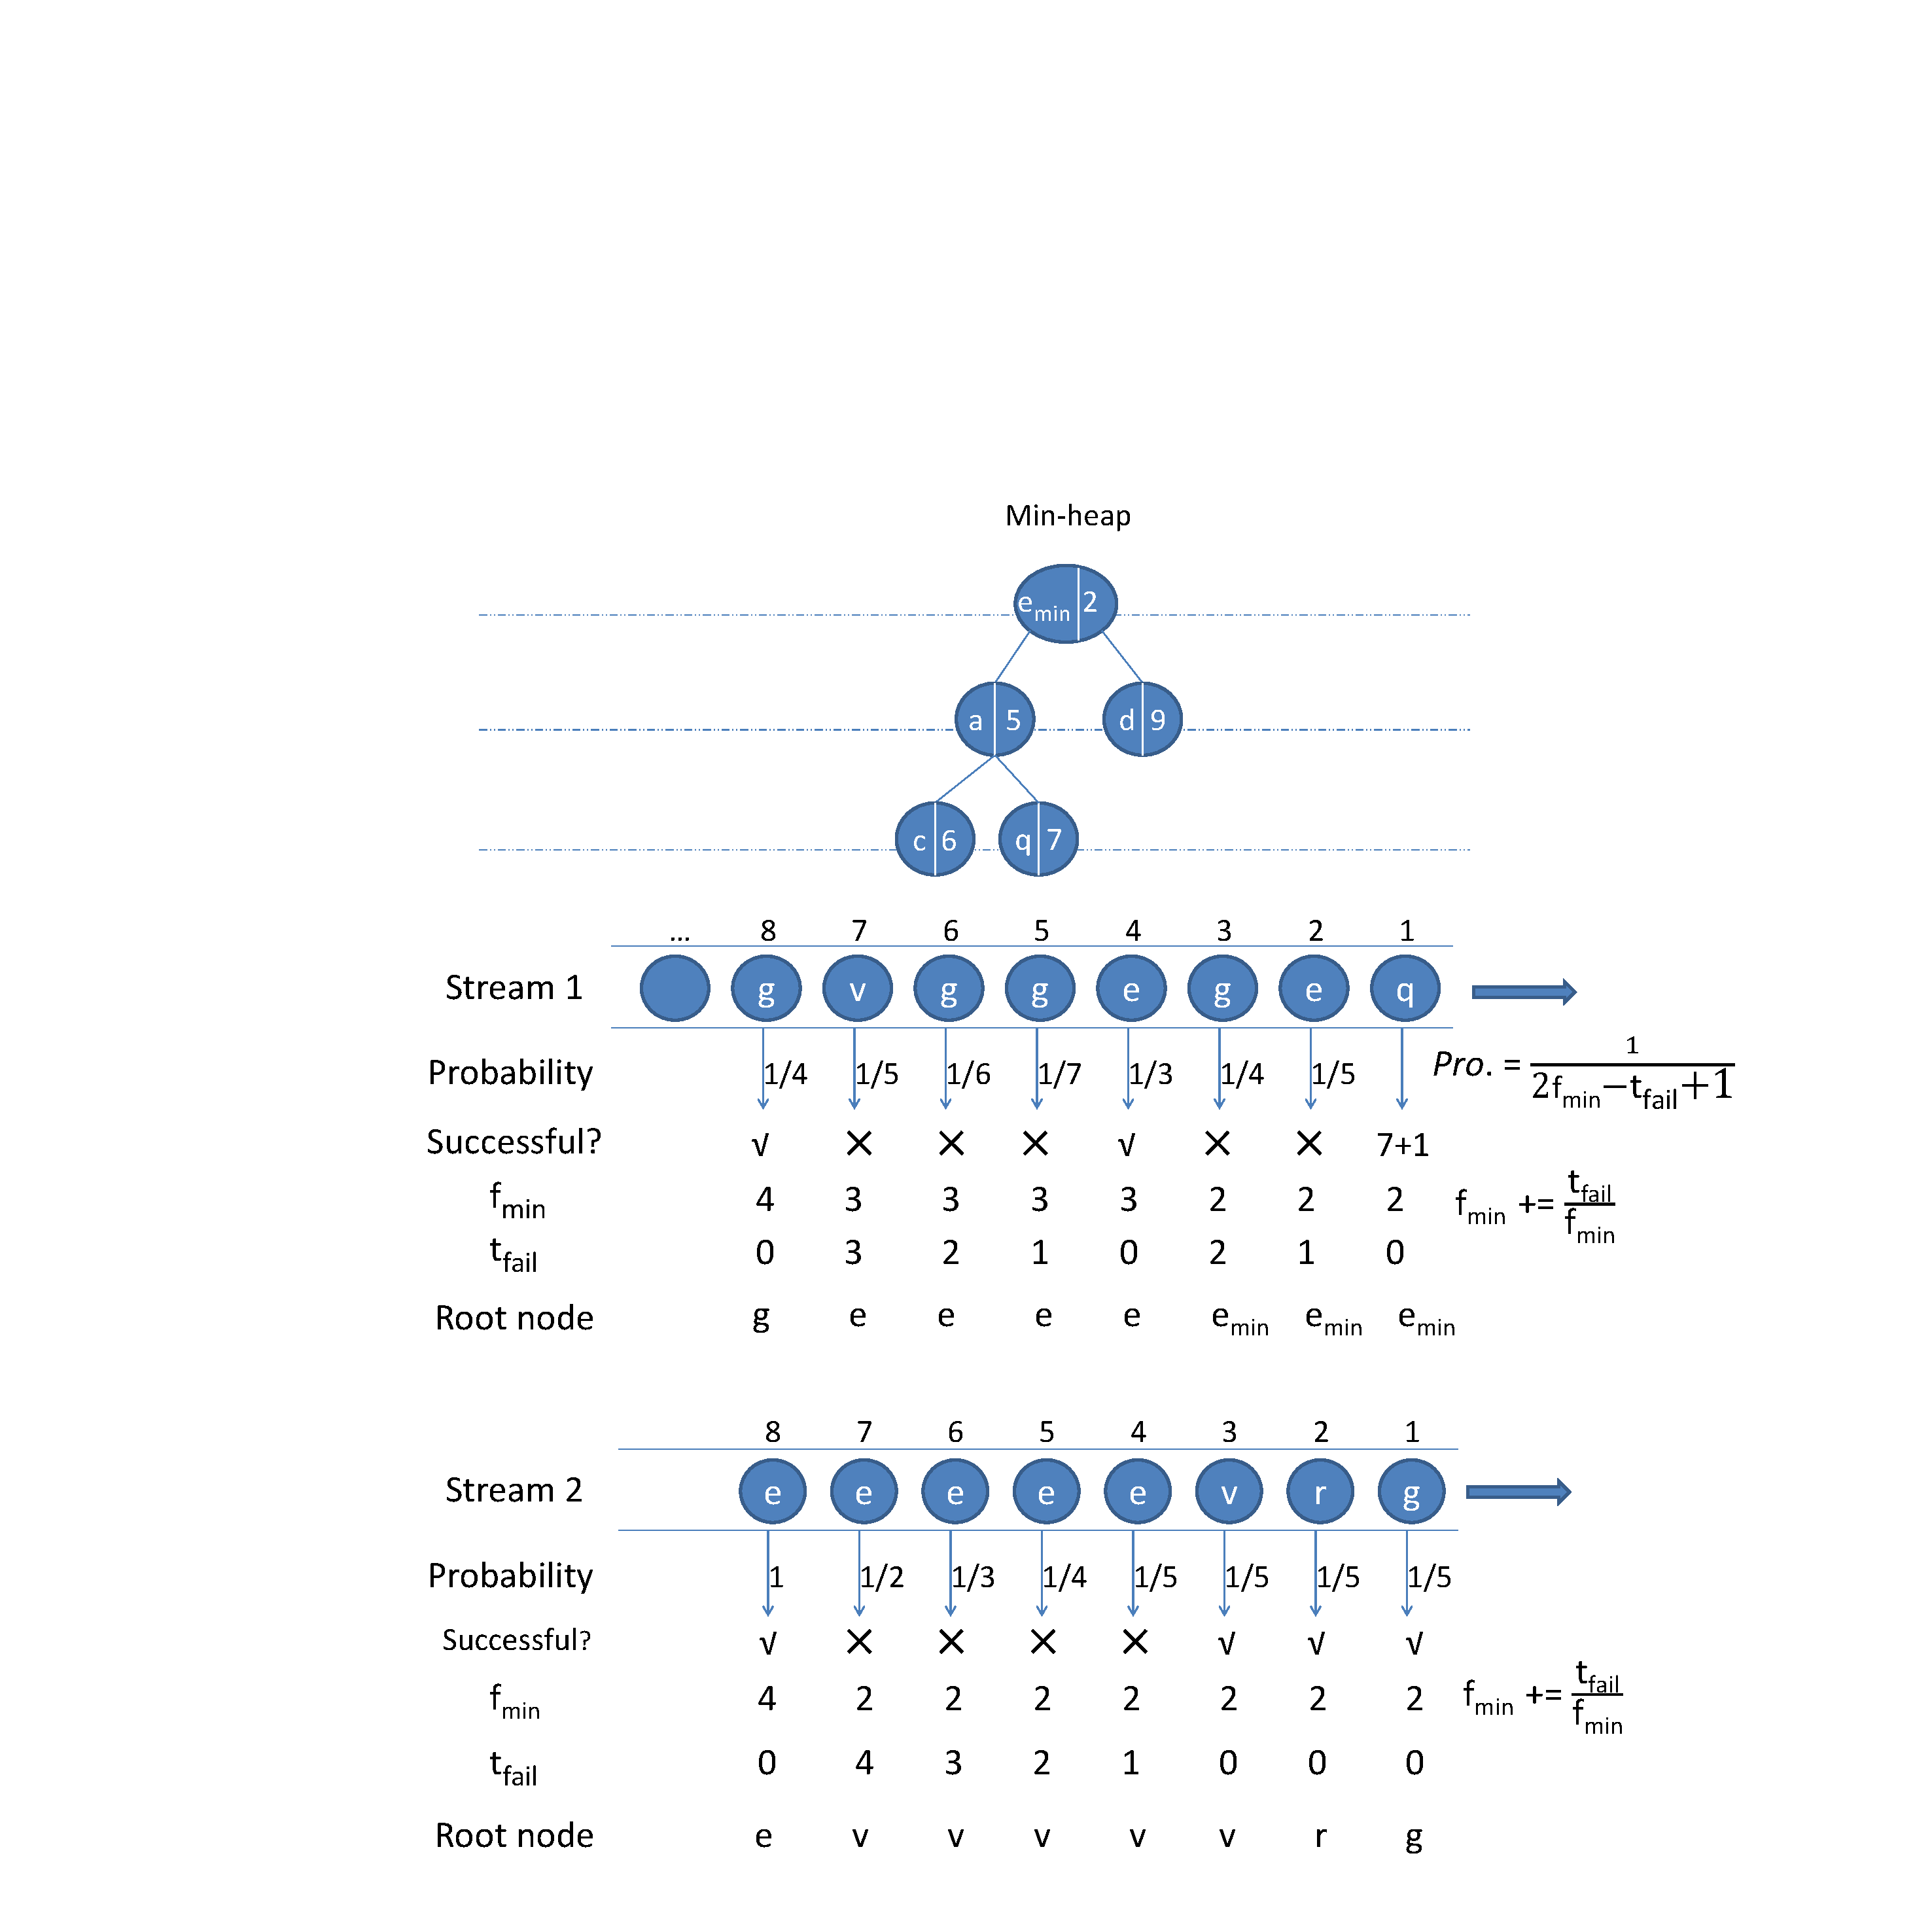
\includegraphics[width=0.5\textwidth]{GraphPPT/example_freq}
	\prefigcaption \vvv\vvv
	\caption{\hl{Examples of PRI when Interest is frequency.}
    }
	\label{draw:freq}
	\postfig \vvv\vvv
\end{figure}
%

\hl{
To clearly show the advantage of PRI, we give two common running examples to show how PRI works. 
Without loss of generality, in these two examples, we let frequency be the interest of items.}
%
\hl{
\mbox{\noindent\textbf{Example 1 (Figure~\ref{draw:freq}):}}
Given a data stream (stream 1): $q,e,g,e,g,g,v,g$, for the first incoming item $q$, we increment the frequency of $q$ in the min-heap by one.
For the following two items $e$ and $g$, replacements fail, and thus $t_{fail}$ is incremented to 1 and then 2. 
The probability increases to 1/3 for the fourth item $e$.
Then $e_{min}$ is successfully replaced by the fourth item $e$ in the root node, and the frequency $f_{min}$ is incremented by $\frac{t_{fail}}{f_{min}}=1$, from 2 to 3, and  $t_{fail}$ is reset to 0.
Since the actual frequency of item $e$ is 2 at present but we record it as 3, the frequency is slightly overestimated.
Then the following 3 items ($g$, $g$, $v$) arrive and replace $e$ with probabilities 1/7, 1/6, and 1/5, but all fail. 
Finally, the eighth item $g$ successfully replaces $e$ and the frequency $f_{min}$ is incremented from 3 to 4, which is exactly the frequency of item $g$ by now in data stream 1. }

\noindent\textbf{\hl{Example 2 (Figure} \ref{draw:freq}):}\hl{
Given another data stream (stream 2): $g, r, v, e, e, e, e, e$, suppose that each of the first three items successfully replaces the root node with the same probability of 1/5, and increments the frequency $f_{min}$ by $\frac{t_{fail}}{f_{min}}(=0)$ each time. 
%
Then item $e$ arrives five times in succession. 
After four unsuccessful replacements with probabilities 1/5, 1/4, 1/3, and 1/2, the eighth item $e$ replaces item $v$ in the root node with probability 1, and increments the frequency $f_{min}$ by $\frac{t_{fail}}{f_{min}}(=2)$, from 2 to 4. 
The frequency $f_{min}$ is slightly underestimated, since item $e$ has appeared 5 times in the data stream by now. 
The first three replacements are wrong, but do not bring a large error to the final value of $f_{min}$. }

\hl{
From the two examples, we see that in our algorithm, the frequency $f_{min}$ might be overestimated or underestimated.
Fortunately, an item might be overestimated at first, but it could be underestimated later, and finally the estimate of the item is probably very close to its true value.
Moreover, successful replacement of infrequent items hardly impact the final result of $f_{min}$.
}

%\xy{$t_{fail}$ of the last e should be 0}

Next, we apply our framework to four specific problems in the following sections.
{
\color{reviewD}
For each problem, we describe the data structure, insertion, and report. Note that we focus only on the variations across the approaches in the specific subsections.
%variation of each problem from the InterestSketch framework.
}



				\presub
\subsection{Finding Frequent Items} \postsub
\label{sub:findfreq}

\ppp{Data Structure (Figure \ref{draw:freq}):}
\aname{} for finding frequent items only uses a min-heap. No filter is necessary since there is no need to remove duplicates. Here the interest is the frequency, \ie, the number of appearances of an item. 

%%
{
\color{reviewD}
\ppp{Insertion:}
The insertion process of the min-heap is exactly the same as that of our framework (see Section \ref{sub:findinterest}).
%The difference is that there is no Bloom filter.
%Given an incoming item, we check whether it is in the min-heap. If the item is in the min-heap, we increment the corresponding frequency by one. Otherwise, if the min-heap is not full, we insert the item into the min-heap. If the min-heap is full, we use the PRI technique.
}

%%
{
\color{reviewD}
\ppp{Report:}
The report process of finding frequent items is exactly the same as that of our framework (see Section \ref{sub:findinterest}).
%To report the items above a given threshold $\mathcal{T}$, we traverse the min-heap to return the items with frequencies larger than $\mathcal{T}$.
}
%
%\begin{figure}[htbp]
%	\centering
%	\prefig
%	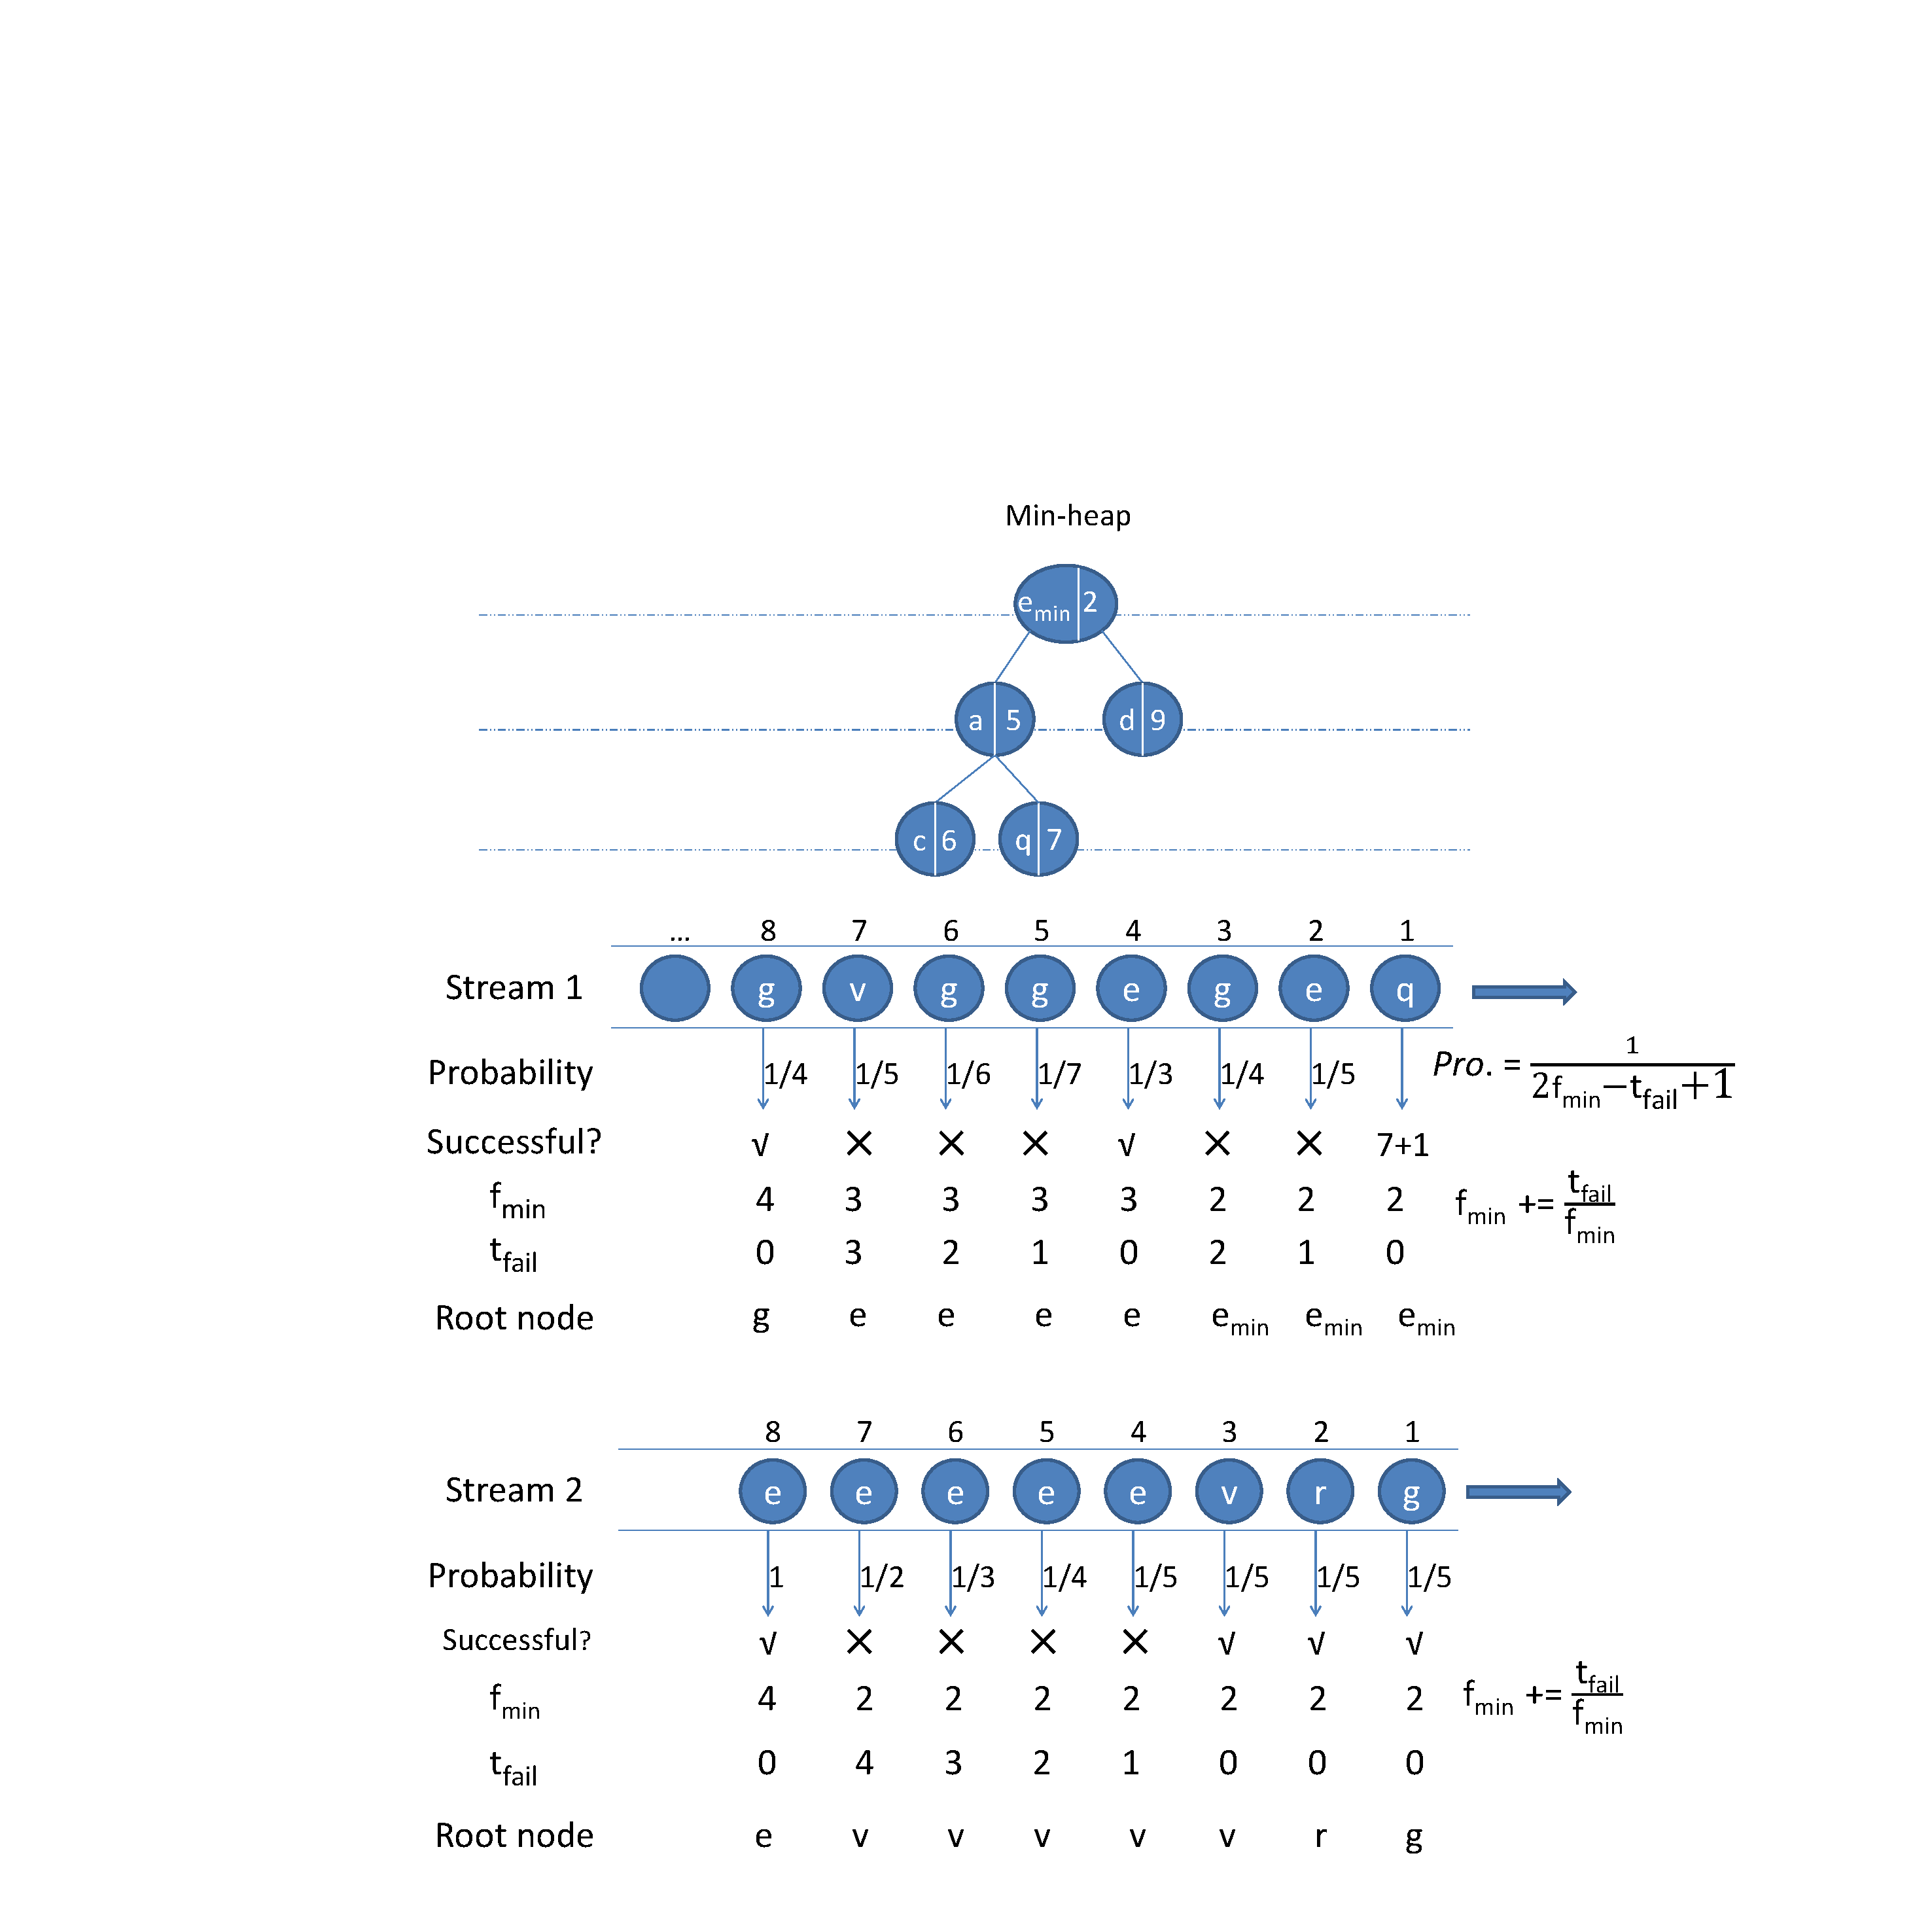
\includegraphics[width=0.5\textwidth]{GraphPPT/example_freq}
%	\prefigcaption \vvv\vvv
%	\caption{\aname{} for finding frequent items.
%
%	\label{draw:freq}
%	\postfig \vvv\vvv
%\end{figure}


%%
%\ppp{Example 1 (Figure~\ref{draw:freq}):}
%%
%Given a data stream (stream 1): $q,e,g,e,g,g,v$ \lar{,g}, for the first incoming item $q$, we increment the frequency of $q$ in the min-heap by one.
%
%For the following two items $e$ and $g$, replacements fail, and thus $t_{fail}$ is incremented to 1 and then 2. The probability increases to 1/3 for the fourth item $e$.
%
%Then $e_{min}$ is successfully replaced by the fourth item $e$ in the root node, and the frequency $f_{min}$ is incremented by $\frac{t_{fail}}{f_{min}}=1$, from 2 to 3, and  $t_{fail}$ is reset to 0.
%
%Since the actual frequency of item $e$ is 2 at present but we record it as 3, the frequency is slightly overestimated.
%
%Then the following 3 items ($g$, $g$, $v$) arrive and replace $e$ with probabilities 1/7, 1/6, and 1/5, but all fail. 
%
%Finally, the eighth item $g$ successfully replaces $e$ and the frequency $f_{min}$ is incremented from 3 to 4, which is exactly the frequency of item $g$ by now in data stream 1. 

%%
%\ppp{Example 2 (Figure \ref{draw:freq}):}
%
%Given another data stream (stream 2): $g, r, v, e, e, e, e, e, e$, \lar{one redundant e} suppose that each of the first three items successfully replaces the root node with the same probability of 1/5, and increments the frequency $f_{min}$ by $\frac{t_{fail}}{f_{min}}(=0)$ each time. \xy{$t_{fail}$ of the last e should be 0}
%
%Then item $e$ arrives five times in succession. 
%
%After four unsuccessful replacements with probabilities 1/5, 1/4, 1/3, and 1/2, the eighth item $e$ replaces item $v$ in the root node with probability 1, and increments the frequency $f_{min}$ by $\frac{t_{fail}}{f_{min}}(=2)$, from 2 to 4. 
%
%The frequency $f_{min}$ is slightly underestimated, since item $e$ has appeared 5 times in the data stream by now. 
%
%The first three replacements are wrong, but do not bring a large error to the final value of $f_{min}$. 

%%
%From the two examples, we see that in our algorithm, the frequency $f_{min}$ might be overestimated or underestimated.
%
%Fortunately, an item might be overestimated at first, but it could be underestimated later, and finally the estimate of the item is probably very close to its true value.
%
%%the average value of the estimator is almost accordant with the actual value, indicating a good unbiasedness of our algorithm. 
%
Moreover, successful replacement of infrequent items hardly impact the final result of $f_{min}$.

%
%%The algorithm is shown in Algorithm~\ref{alg:fre} in Appendix~\ref{sec:appendix}.
%The detailed description of the algorithm is similar to Algorithm \ref{alg:basic}.

                \presub
\subsection{Finding Heavy Changes}
\postsub

\ppp{Rationale:} 
Both heavy changes and frequent items are related to the frequencies of items.
%
One typical approach for finding heavy changes is to build two data structures for frequent items in two periods respectively.
%
Our algorithm also uses this approach.
%
%The accuracy of this method highly depends on the accuracy of heavy hitters.


\ppp{Data Structure:}
For each period, we only build a min-heap, and do not use the filter. This min-heap is used to record frequent items.

{
\color{reviewD}
\ppp{Insertion:} For each period,
the insertion process of the min-heap is exactly the same as that of our framework (see Section \ref{sub:findinterest}).
}


\ppp{Report:} For two adjacent periods, we traverse all items: for each item, we query its frequency in the two min-heaps, and get two frequencies. If the difference of the two frequencies is larger than a predefined threshold, the item is reported as a heavy change. Note that if an item only appears in one min-heap, the queried frequency of the other min-heap is 0.

\ppp{Analysis:}
All algorithms for finding frequent items can be used for finding heavy changes.
%
There are three metrics for finding frequent items: precision, recall, and the accuracy of the estimate of the reported items.
Only if all three metrics are high, the error of heavy changes is small. Fortunately, InterestSketch is accurate in terms of all three metrics, and thus can achieve very high accuracy for finding heavy changes.
%
%However, some algorithms for frequent items only focus on the precision or recall, but the accuracy for frequency 








				\vvv\vvv\vvv
\presec
\subsection{Finding Super-spreaders} \postsec
\label{sec:basicAlgorithm:SS}

\ppp{Data Structure:}
In the data structure of InterestSketch for finding super-spreaders, both of the filter and the min-heap are used.  

For a given source IP address, we need to count the number of connections, \ie, the number of different destination IP addresses. 
%
If the source IP address sends more than one packet to a specific destination IP address, we increment the value of connection for only the first packet (but not for the other packets as these are duplicates in this case).
%
{
\color{reviewD}
%The Bloom filter is used for de-duplication before inserting items into the min-heap. 
We remind readers that details about Bloom filters are provided in Section~\ref{sub:findinterest}.
}


%
Each node in the min-heap stores two fields: the source IP address (ID) as key, and the \textit{connection} as value. 
%
The root node in the min-heap stores the source IP with the smallest connections.

{\color{reviewD}
\ppp{Insertion:}
The insertion process of finding Super-Spreaders is similar to that of our framework (Section \ref{sub:findinterest}).
%Given an incoming packet $e$, there are two steps. First we check the Bloom filter to judge whether $e$ is a duplicate. Second, if the Bloom filter reports true, $e$ is discarded. Otherwise, we try to insert $e$ into the min-heap.
There are two differences.
First, when checking or querying the Bloom filter, the item ID is the source IP address plus the destination IP address.
Second, when checking or updating the min-heap, the item ID is the source IP address only.
%Specifically, given an incoming packet $e$ (with ID of source+destination), we first check the Bloom filter by calculating the $z$ hash functions and get $z$ \textbf{\textit{hashed bits}}. 
%If all the $z$ hashed bits are 1, the packet is probably not the first one sent from the source to the specific destination, and it is discarded. 
%If the $z$ hashed bits are not all 1s, $e$ is definitely the first packet from the source to the destination. In this case, we first set all the $z$ bits to 1, and then try to insert $e$ (with ID of source only) into the min-heap. There are two cases: 1) If the source IP address of the packet is in the min-heap, we increment the corresponding connection. 2) Otherwise, if the min-heap is not full, we simply insert this source IP address into the min-heap. If the min-heap is full, we try to insert the source IP address into the root node by using our PRI algorithm.
}

{\color{reviewD}
\ppp{Report:}
The process of reporting Super-Spreaders is similar to that of Section \ref{sub:findinterest}.
%To report the source IP addresses above a given threshold $\mathcal{T}$, we traverse the min-heap to pick the source IP addresses with connection larger than $\mathcal{T}$.
}

\begin{comment}
\begin{figure}[htbp]
	\centering
	\prefig
	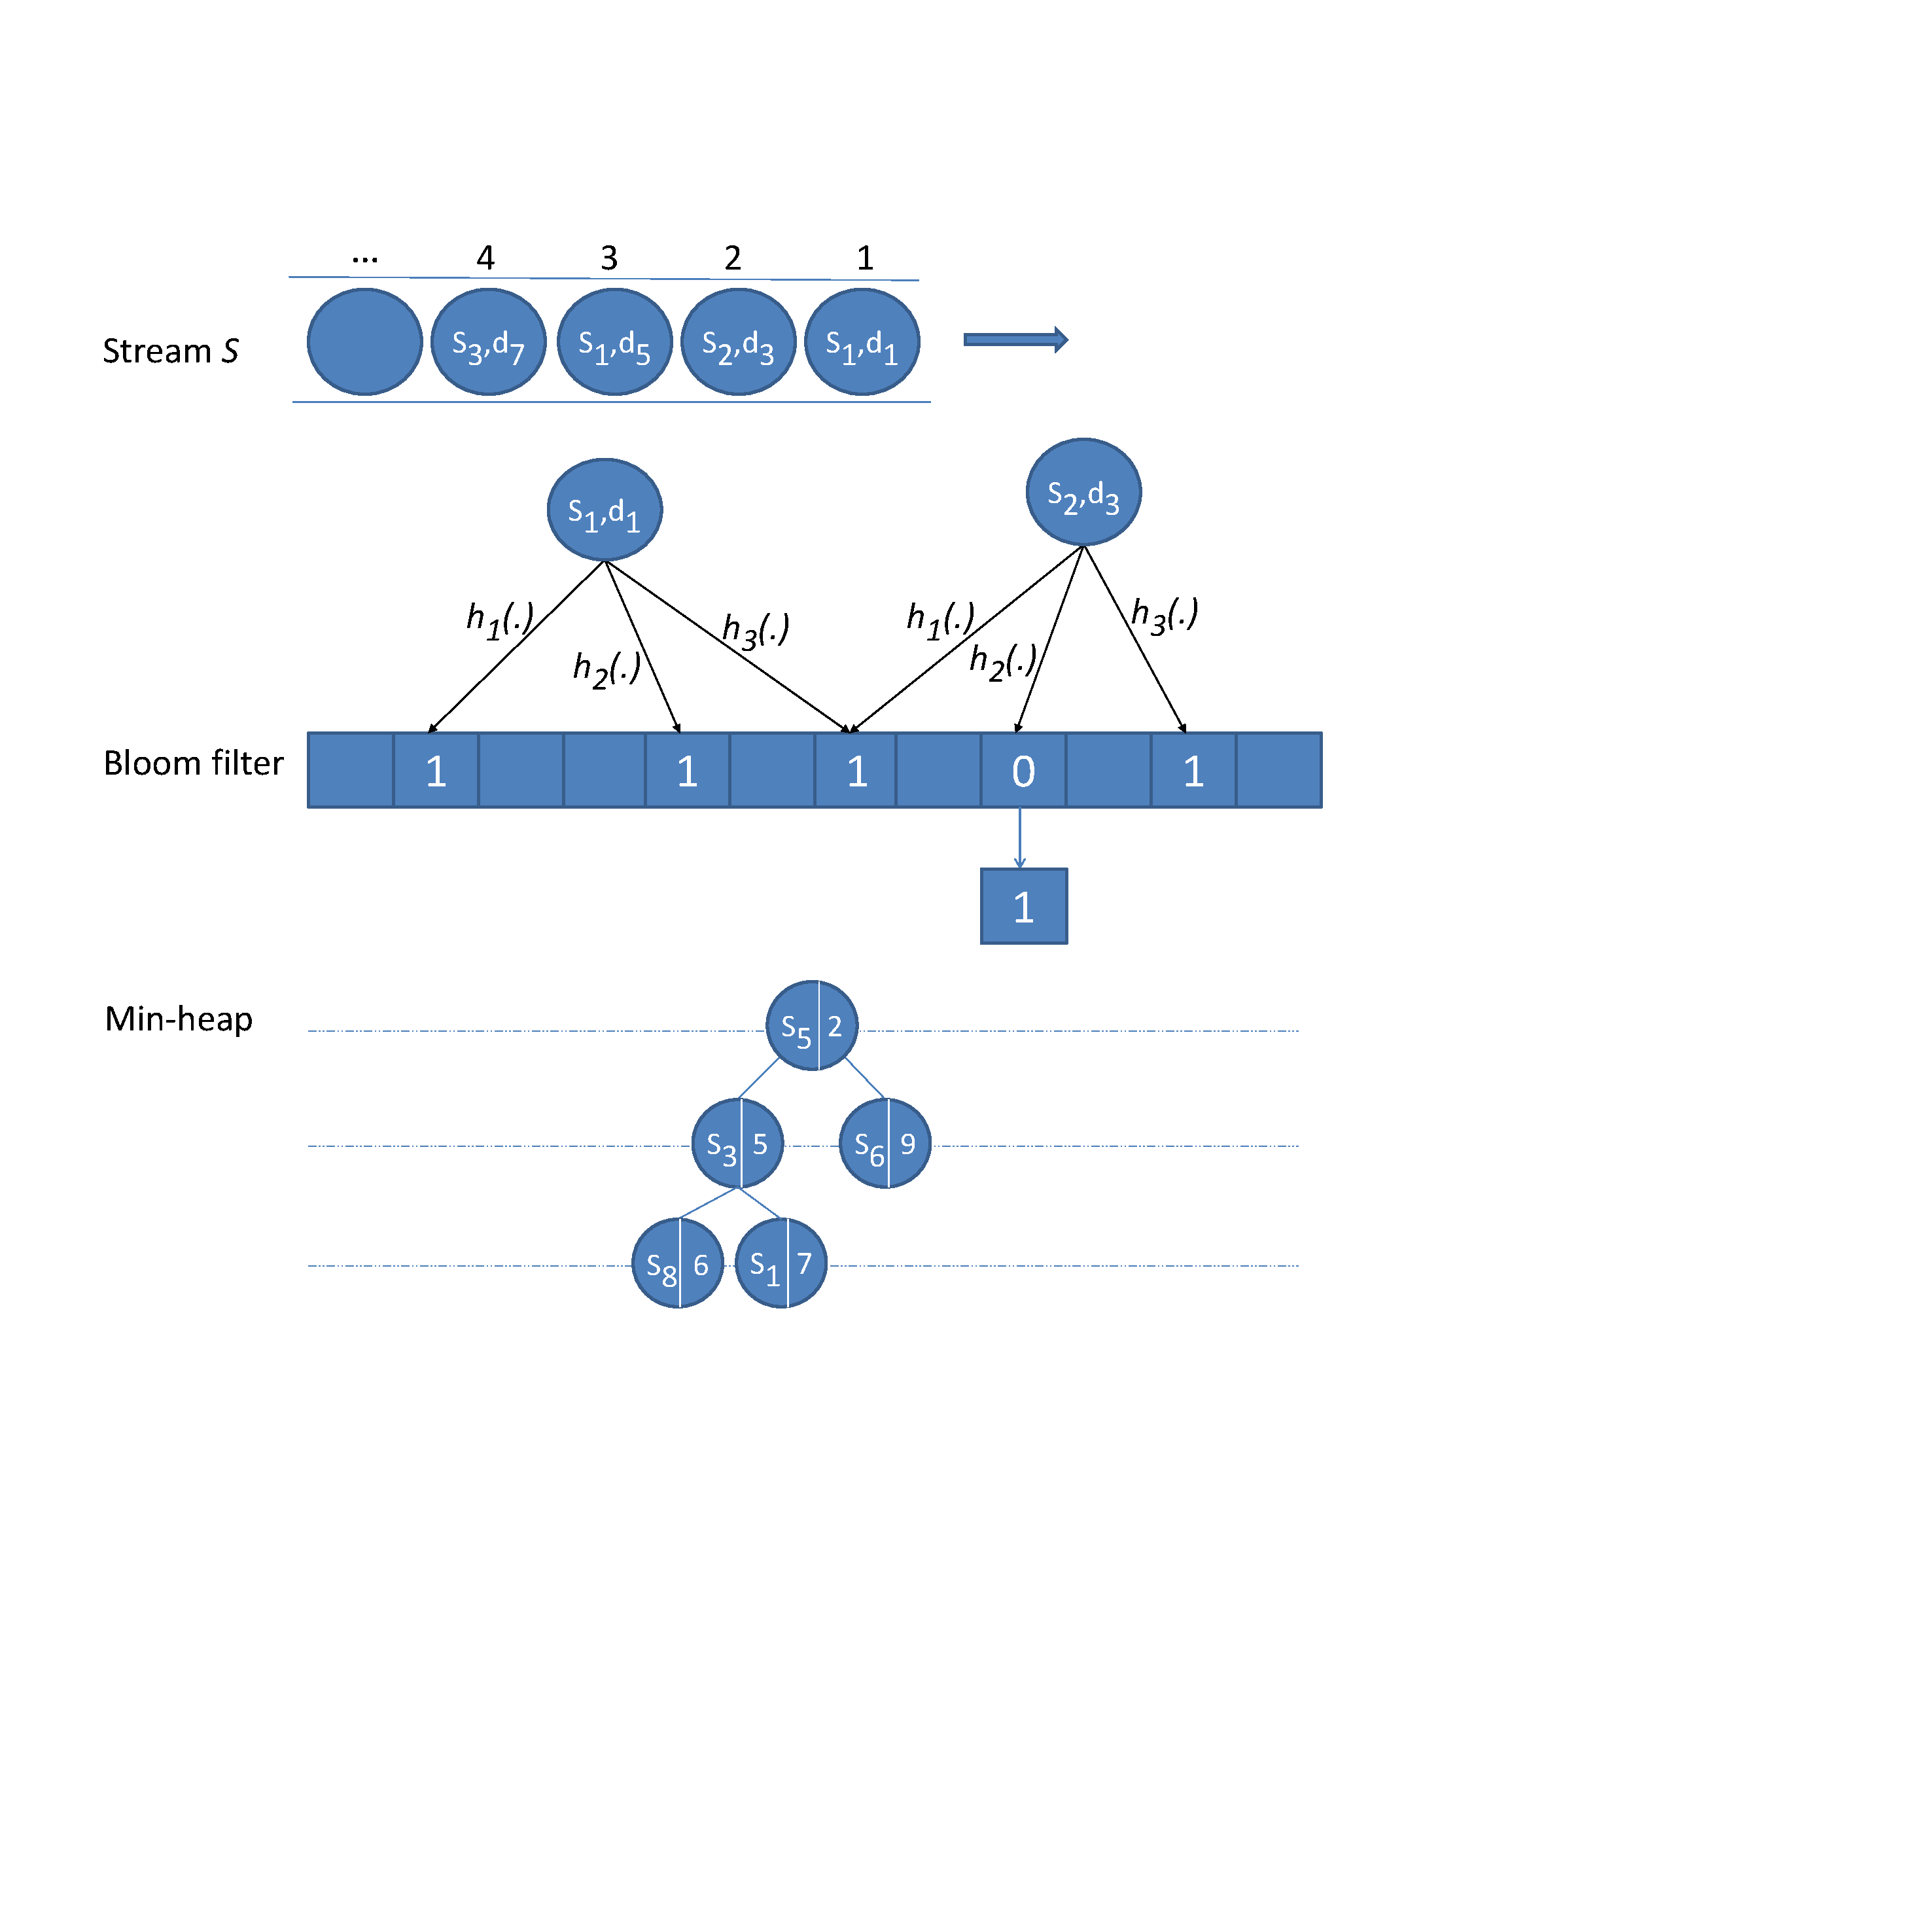
\includegraphics[width=0.5\textwidth]{GraphPPT/example_SS}
	\prefigcaption \vvv\vvv\vvv
	\caption{\aname{} for finding super-spreaders.}
	\label{draw:SS}
	\postfig \vvv\vvv \vvv\vvv
\end{figure}

\ppp{Example:}
As shown in Figure~\ref{draw:SS}, in the min-heap, the source IP address is stored in each node as the item ID. 
%
Given a network stream, each packet has a source IP address ($s_i$) and a destination IP address ($d_i$). 
%
For the first incoming packet with ($s_1,d_1$), we calculate three hash functions $h_1(s_1,d_1),h_2(s_1,d_1),~and~h_3(s_1,d_1)$. 
%
If all of three \textit{hashed bits} are $1$, indicating that this packet is not the first one sent from $s_1$ to $d_1$, we discard it. 
%
When the second packet with ($s_2$, $d_3$) arrives, one of the three hashed bits is $0$, indicating that this packet is the first one sent from $s_1$ to $d_3$ and $s_1$ is not in the min-heap. 
%
We change the second hashed bit from $0$ to $1$ in the Bloom filter and then insert $s_2$ into the min-heap, by applying our PRI algorithm (see Section \ref{sub:findfreq}). 
%
In this way, the source IP addresses with the largest connection (\ie, number of destination IP addresses) are recorded in the min-heap. 
%
%The algorithm is shown in Algorithm~\ref{alg:sup} in Appendix~\ref{sec:appendix}.
%
The detailed description of the algorithm is similar to the basic Algorithm.
%~\ref{alg:basic}.

\end{comment}
				\vvv\vvv\vvv
\presec
\subsection{Finding Persistent Items} \postsec
\label{sec:basicAlgorithm:persistent}

{\color{reviewD}
\ppp{Data Structure:}
The data structure of \aname{} of finding persistent items is exactly the same as that of our framework (Section \ref{sub:findinterest}): a Bloom filter and a min-heap. 
%The Bloom filter is used to remove duplicates in each period. 
%Each node of the min-heap stores an item ID and the corresponding persistency. 
%The root node stores the item with the smallest persistency. 
}


{\color{reviewD}
\ppp{Insertion:}
The insertion process of finding persistent items is similar to that of our Framework (see Section \ref{sub:findinterest}).
Here Bloom filter is used to check whether the item has probably been recorded in the current period.
The only difference is that we need to periodically empty the Bloom filter in this task.
%Given an incoming item, we first check the Bloom filter by calculating the $d$ hash functions. If the $d$ hashed bits are all 1, indicating that the item has probably been recorded in this period, we just discard the item. If the $d$ hashed bits are not all 1, we first set all the $d$ bits to 1. 
%
%Then, there are two cases: 1) If the item is in the min-heap, we increment the corresponding persistency by one. 2) Otherwise, the item is not in the min-heap, and if the min-heap is not full, we insert this item into the min-heap. If the min-heap is full, we try to insert the item into the root node using our PRI algorithm.
}


\ppp{Periodically Emptying:}
At the end of each period, we empty the Bloom filter by setting all bits to 0. In other words, the Bloom filter is used to indicate whether an item appears in the current period only.


{\color{reviewD}
\ppp{Report:}
The process of reporting persistent items is exactly the same as that of our framework (Section \ref{sub:findinterest}).
%To report all the items above a given threshold $\mathcal{T}$, we traverse the min-heap to pick out the items with persistencies larger than $\mathcal{T}$.
}

\begin{comment}

\begin{figure}[htbp]
	\centering
	\prefig
	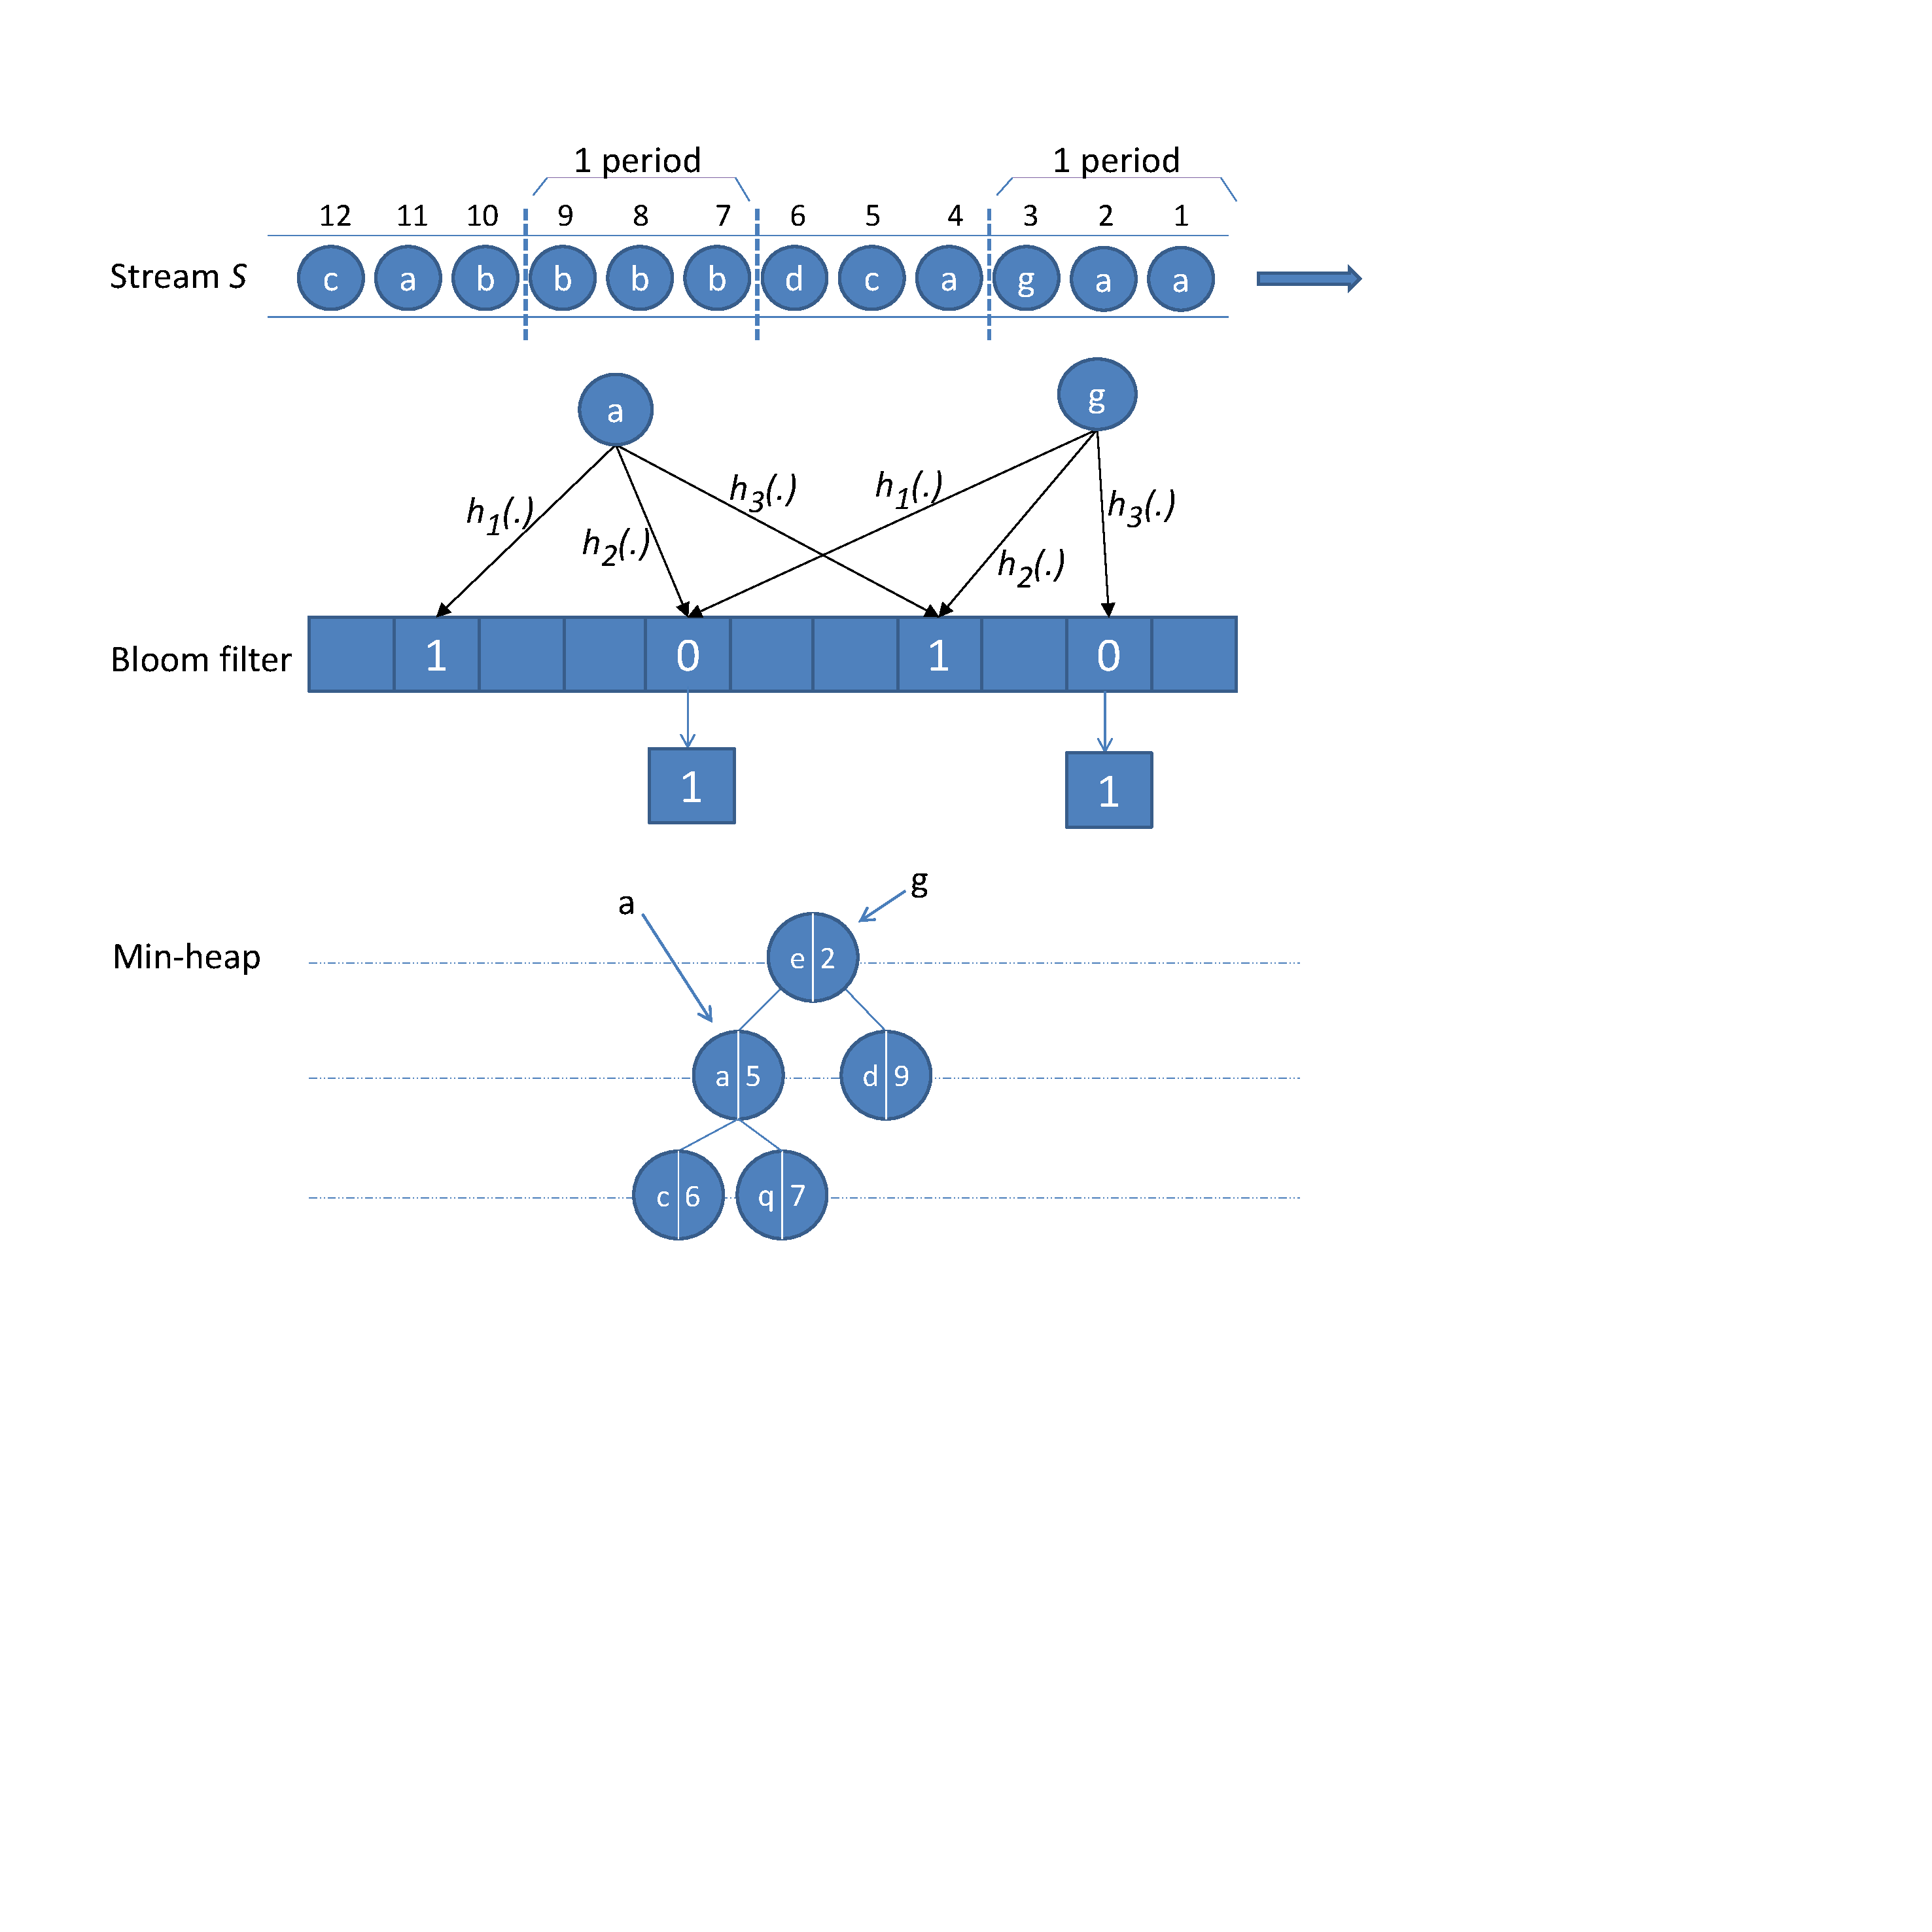
\includegraphics[width=0.5\textwidth]{example_per}
	\prefigcaption\vvv\vvv
	\caption{\aname{} for finding persistent items.}
	\label{draw:persistency}
	\postfig \vvv\vvv
\end{figure}

\ppp{Example:}
As shown in Figure \ref{draw:persistency}, for a given data stream, we divide them into multiple equal-sized periods. 
%
For the first incoming item $a$, we get the three hashed bits ($1,0,1$), which means that item $a$ has not been recorded in the min-heap in this period. 
%
Therefore, we change the hashed bit from $0$ to $1$ in the Bloom filter and increment the persistency of $a$ by one in the min-heap. 
%
Next we calculate three hash functions $h_1(a),h_2(a),h_3(a)$ for the second incoming item $a$. 
%
The three hashed bits are all $1$, which indicates that $a$ has been recorded in this period and thus the second item $a$ is discarded. 
%
When the third item $g$ arrives, the third hashed bit is $0$, so we insert $g$ into the min-heap and change the third hashed bit from $0$ to $1$.
%
Since $g$ is not in the min-heap, we try to insert it into the root node by applying our PRI algorithm. 
%
At the end of each period, we empty the Bloom filter by setting all bits to $0$. 
%
In this way, when the fourth item $a$ arrives in the next period, the persistency of $a$ in the min-heap can be incremented by one regardless of the record in the previous period.
\end{comment}

%
%The algorithm is shown in Algorithm~\ref{alg:per} in Appendix~\ref{sec:appendix}.
%
%The detailed description of the algorithm is similar to Algorithm~\ref{alg:basic}.

\presub
\subsection{{\color{reviewD}For Hopping Windows and Sliding Windows}}
\postsub


{\color{reviewD}
Our algorithm can also be used for hopping windows and sliding windows.
%handle the problems with a small change. 
As for hopping windows, we need a InterestSketch for each window. As for the overlap between the windows, an item may need to be checked in many InterestSketchs. Once a window runs out of time, the InterestSketch should be immediately set to zero, and it can be used for a new window. Therefore, the memory overhead will be $k-1$ more InterestSketch than the original algorithm. The sliding window is a special case of hopping window with a very large $k$. We also can handle the sliding window with more memory overhead.}



\vvv
\presub
\subsection{Shortcomings of the Basic Version}
\postsub

Our basic version has the following two shortcomings.
%
%First, when judging whether an item is in the min-heap, the whole heap should be traversed with the time complexity of $O(k)$, where $k$ is the number of items in the min-heap. 
%
First, we need to check whether every incoming item is in the min-heap, and the time complexity is $O(k)$, where $k$ is the number of items in the min-heap. 
%
This problem can be solved by adding a hash table. However, the hash table will inevitably bring hash collisions and a waste of memory space. 
%
Second, when updating the min-heap, the time complexity is $O(logk)$. Since the speed of data streams is often high, we wish to reduce the time complexity from $O(logk)$ to $O(1)$.
	\presec \vvv
\section{Optimizations: Final Version} \postsec
\label{sec:optimization}
\label{sec:final}

To address the two shortcomings of our basic version, we propose an optimization method. 
For convenience, and without loss of generality, \textit{we assume the interest is frequency in this section}. When interest is defined as change of frequency, persistency or connection, the optimization remains unchanged. 
%In practice, we recommend using our final version of storing multiple items in one bucket, because it overcomes all shortcomings of the previous versions.
%(see Section \ref{sec:final}).
%^and related experiments are shown in Appendix~\ref{eva_para}.


\begin{comment}

%\presub \vvv\vvv
%\subsection{Using Stream-Summary}
\postsub

The basic version of our algorithm is slow with insertions. 
%
To address this, we accelerate our algorithm by replacing the min-heap with Stream-Summary\cite{spacesaving} and a hash table. 
%
Stream-Summary is a data structure proposed by the authors of SpaceSaving~\cite{spacesaving}. 
%
It can achieve $O(1)$ time complexity for both updating the heap and returning the smallest item. 
%
Stream-Summary is a double-directional linked list consisting of nodes.
%
Each node stores a unique frequency. 
%
For a given node with frequency $f$, it has a linked list storing all the items whose frequency is exactly $f$.
%
In the hash table, the key is the flow ID, and the value is a pointer to the corresponding node in the min-heap.
%
The hash table is used to check whether the incoming flow is in the Stream-Summary, and if so, the corresponding frequency will be incremented by 1.


However, this optimization has inevitable drawbacks.
%
First, Stream-Summary consumes a relatively large amount of memory, since it is a double-directional linked list and each node has four or six pointers. 
%
Second, the hash table also requires a significant amount of memory space to minimize the hash collision rate. 
%
Third, the update process is relatively slow because multiple pointers need to be modified for each update.
\end{comment}

\begin{comment}
\presub
\subsection{Using Multiple Arrays} \postsub
\label{sec:multi:array}

To solve the problem of memory space consumption in the previous optimization, we propose another optimization using multiple arrays. 

\begin{figure}[htbp]
	\centering
	\prefig
	%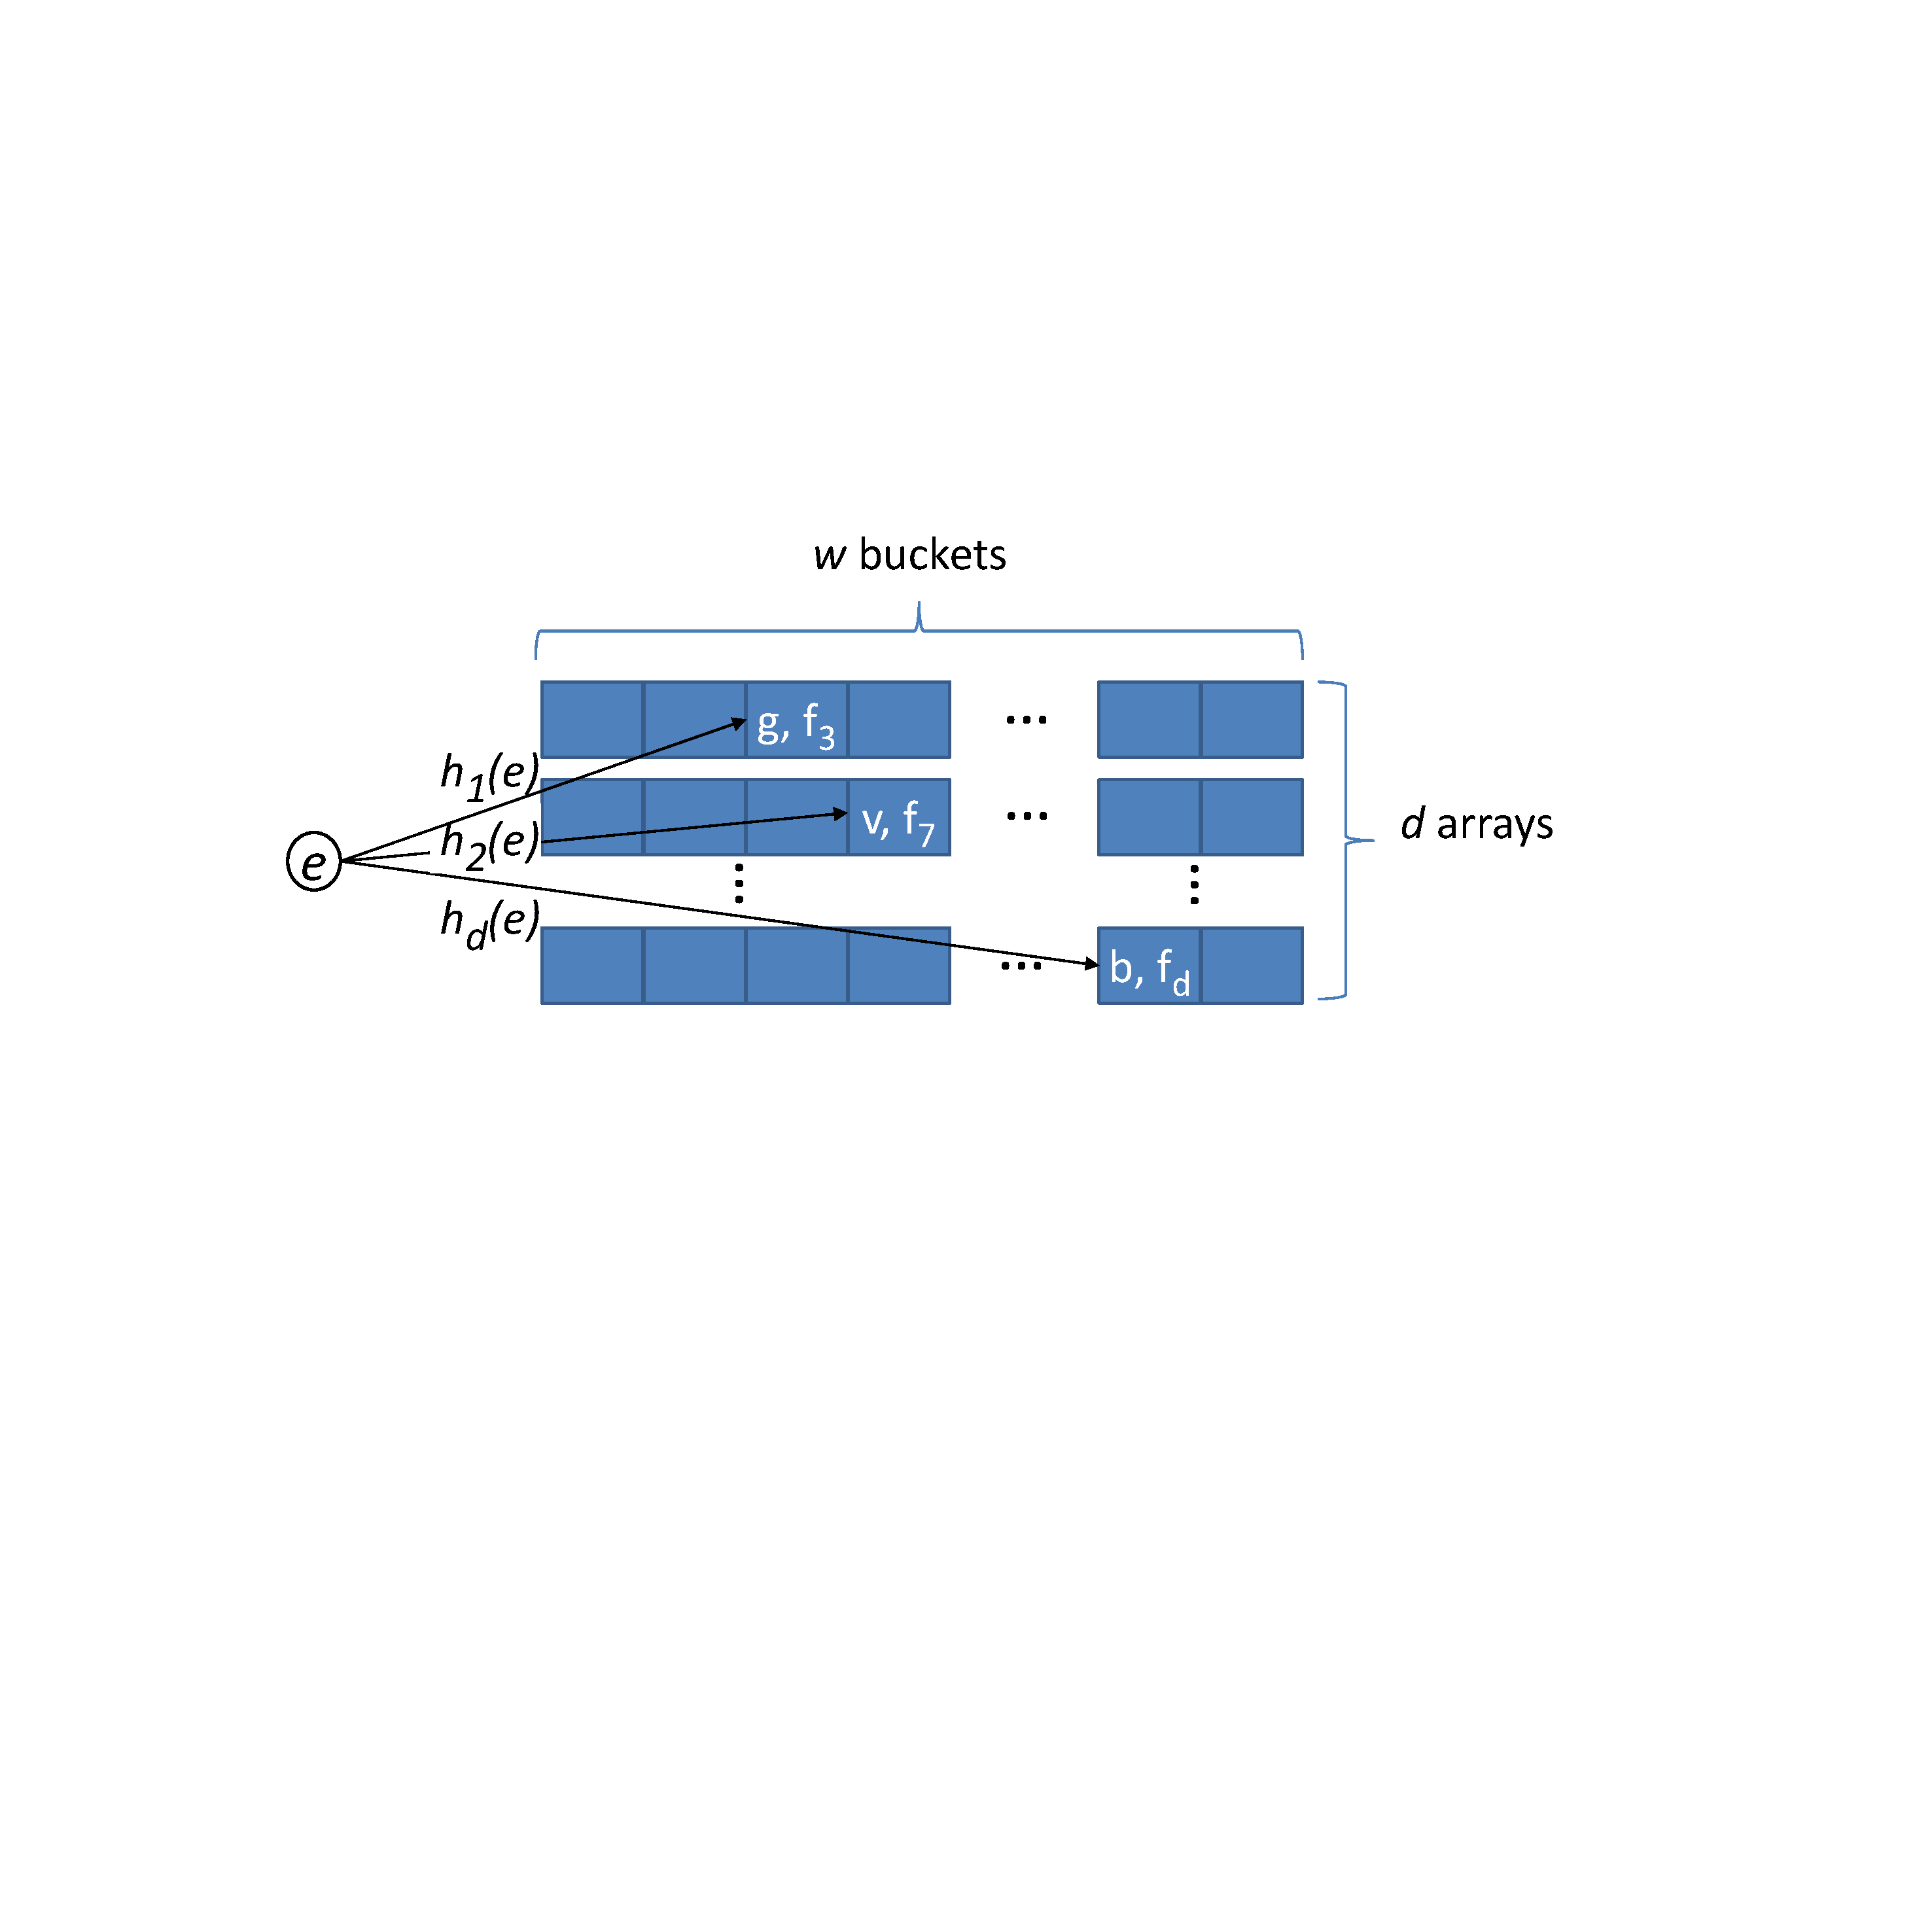
\includegraphics[width=0.49\textwidth]{mul_array}
	\prefigcaption
	\caption{\aname{} using multiple arrays.}
	\label{draw:mul_array}
	\postfig
\end{figure}

\ppp{Data Structure (Figure~\ref{draw:mul_array}):}
There are $d$ arrays in total and each array corresponds to a hash function. 
%
Each array consists of $w$ buckets and each bucket stores the ID and frequency of an item. Every bucket has its own $t_{fail}$.

\ppp{Insertion:}
%For an incoming item $e$, we calculate $d$ hash functions and pick the corresponding $d$ buckets.
%
There are three cases. First, if one of the $d$ buckets stores the item with the same ID as the incoming item $e$, we increment the frequency in that bucket. 
%
Second, if there is no item with the same ID as $e$ but there are empty buckets, we just store $e$ in the first empty bucket. 
%
Third, if there is neither item with the same ID nor empty buckets, we select the bucket with the smallest frequency and replace the original item with the incoming one using our PRI algorithm. 

 \ppp{Query:}
 For a given item $e$, to find its frequency, we just calculate $d$ hash functions and pick out the corresponding $d$ buckets.
% %
 If there is an item with the same ID as $e$ in any one of the $d$ buckets, the frequency stored in that bucket is returned. Otherwise, we report false.

\ppp{Report:}
%To return the items with frequency larger than a predefined threshold $\mathcal{T}$, we traverse the $d$ arrays. 
%
If the frequency stored in a bucket is larger than $\mathcal{T}$, the corresponding item is reported.

 \ppp{Deletion:}
 Given the ID of an item, to delete that item from our data structure, we calculate $d$ hash functions. If the item with the same ID exists, we decrement the frequency by one. Otherwise, the data structure remains unchanged.

\ppp{Advantages and Disadvantages:}
Compared with the memory hungry Stream-Summary, using multiple arrays minimizes the memory usage thanks to the following two reasons.
%
First, there is no pointer in this data structure. Second, since the number of items is far larger than that of buckets, there are few, if any, empty buckets.
%
Given the same memory space, using multiple arrays outperforms Stream-Summary to a large extent in terms of accuracy.  
%
However, the time complexity of insertions is $O(d)$, where $d$ is the number of arrays. 
%
Although $d$ can be small (\eg, 3 or 4), we still wish to reduce the time complexity to $O(1)$, without sacrificing accuracy or memory efficiency. 
%
Therefore, we propose the final optimization in the following subsection.
\end{comment}

%\presub\vvv
%\subsection{Final Version: Storing Multiple Items in one Bucket} \postsub

%\ppp{Final Version: Storing Multiple Items in one Bucket}
%We recommend this final version for finding interesting items, because it overcomes all shortcomings of the previous versions.
 
 \begin{figure}[htbp]
	\centering
	\prefig \vspace{-0.05in}
	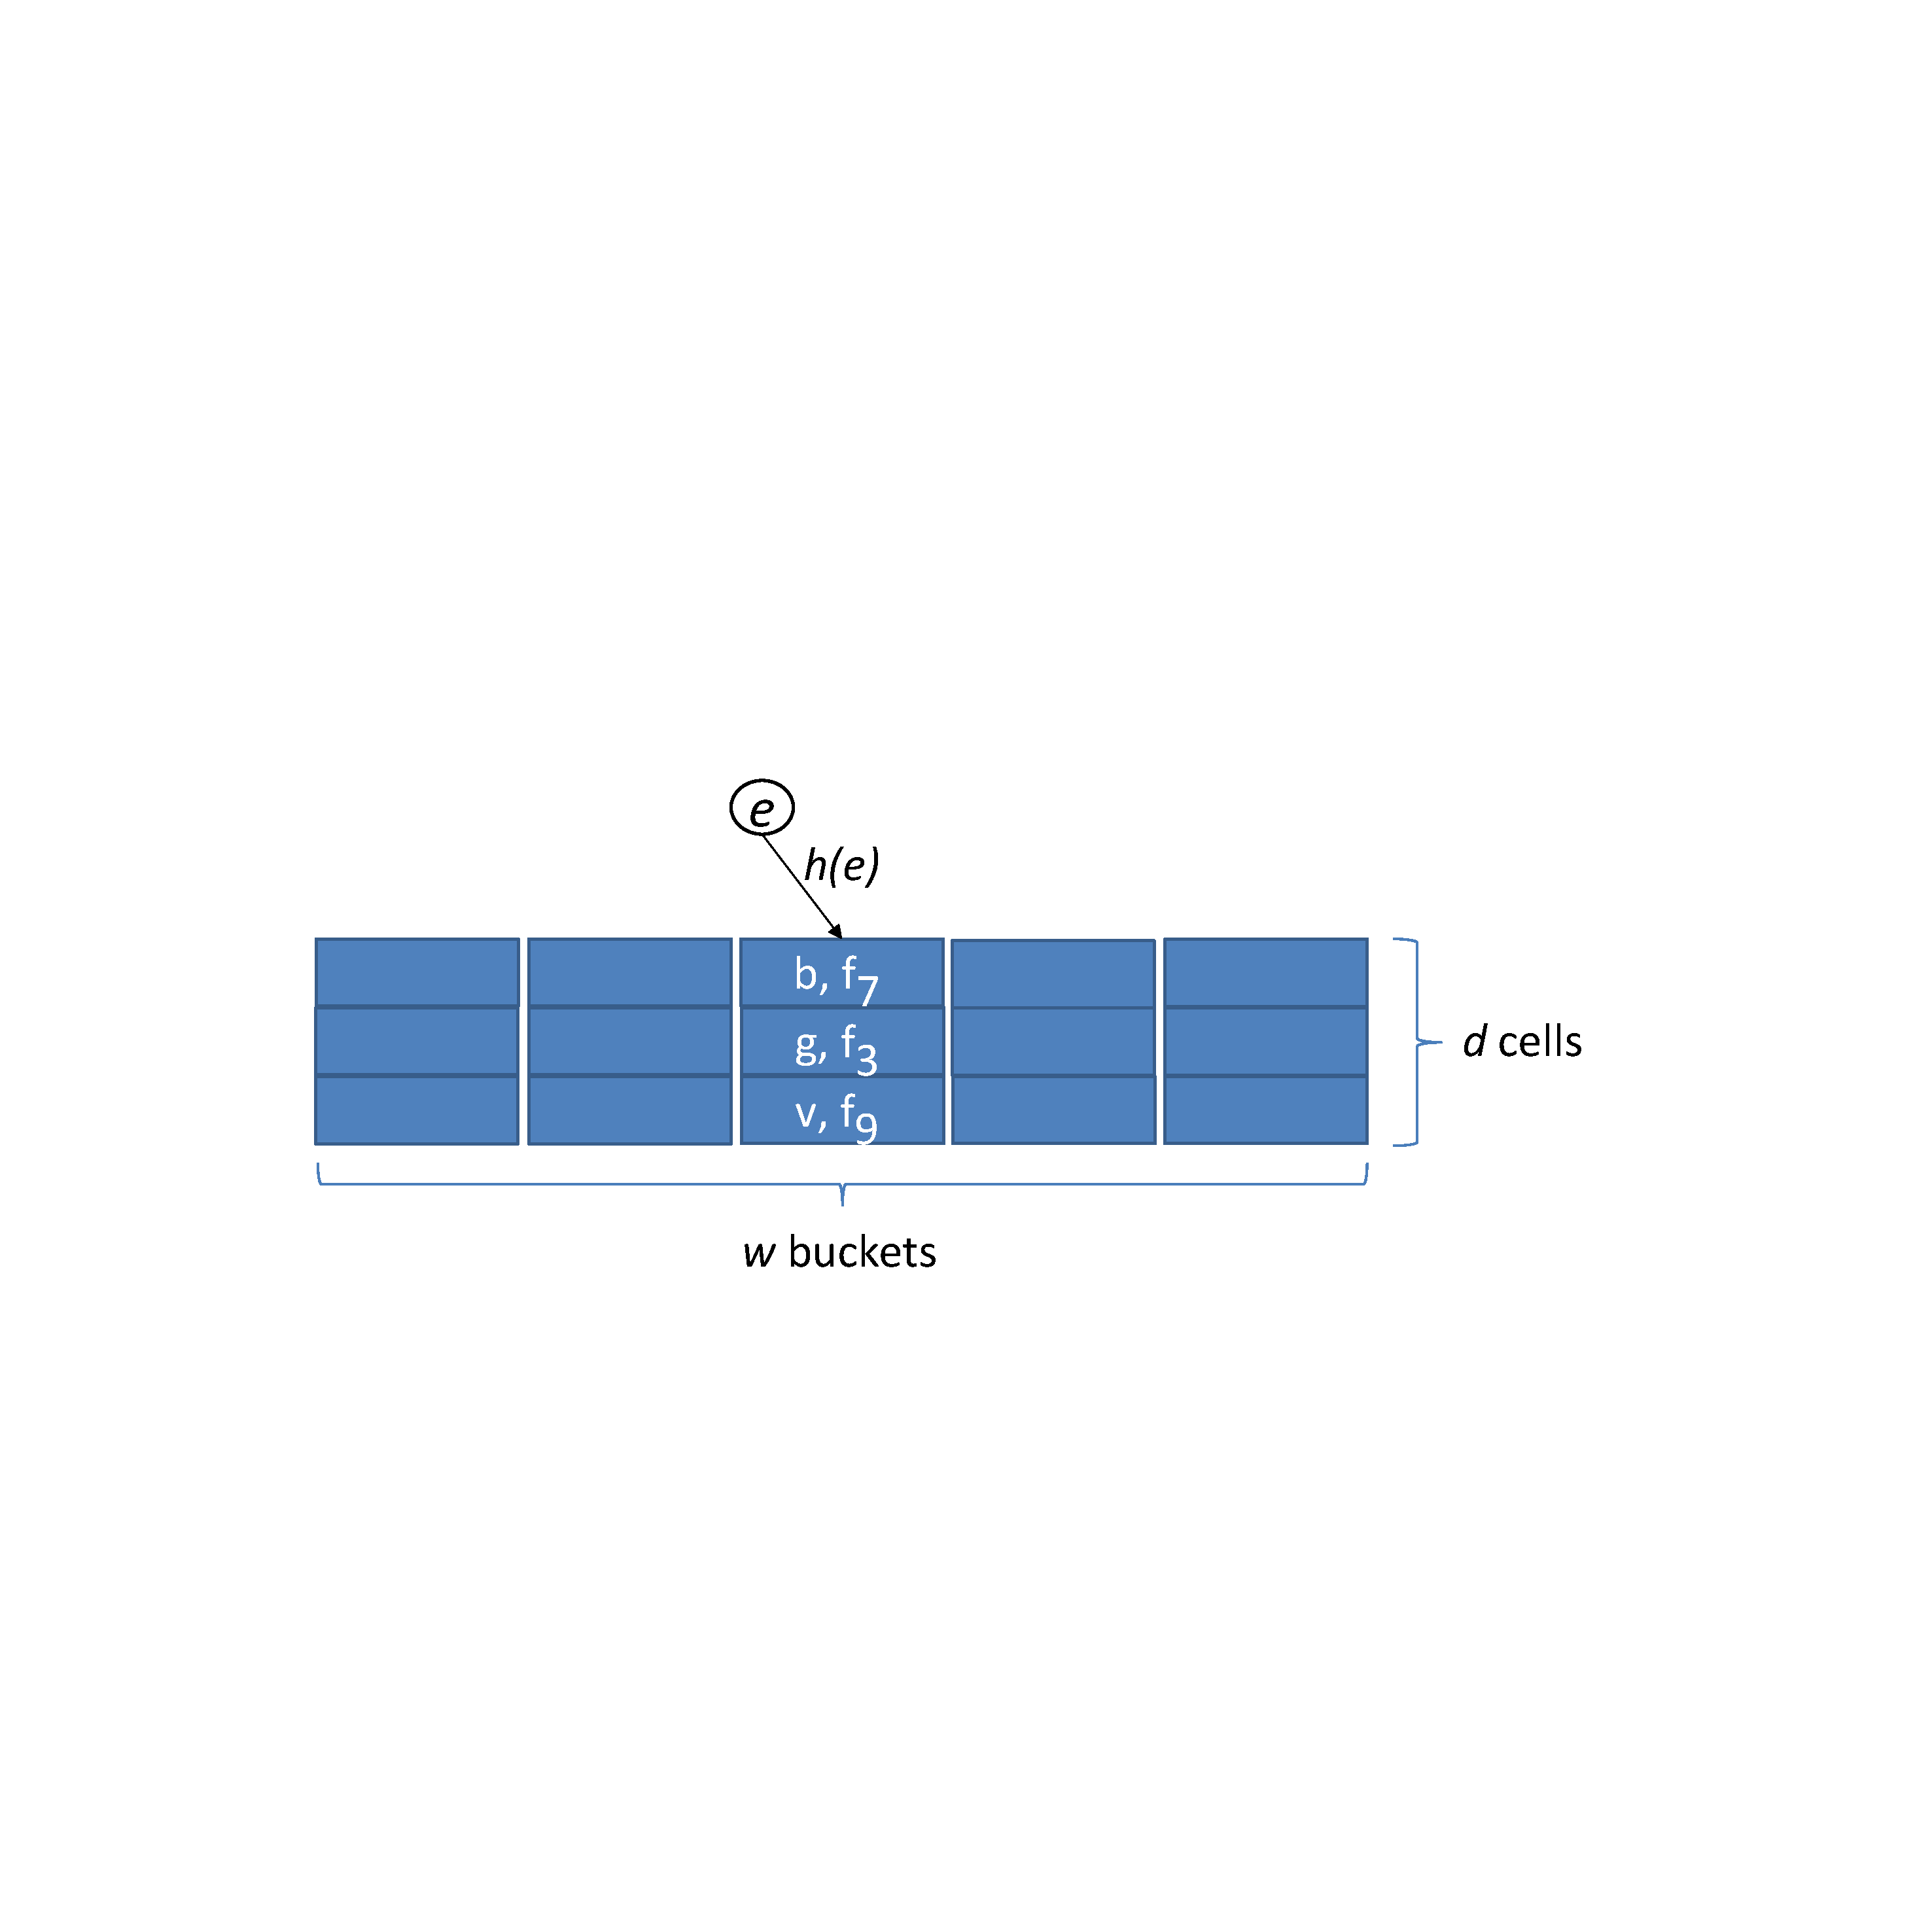
\includegraphics[width=0.48\textwidth]{mul_cell}
	\prefigcaption \vspace{-0.05in} \vspace{-0.05in}
	\caption{\aname{} using multiple cells in every bucket.}
	\label{draw:mul_cell}
	\postfig \vspace{-0.05in}
\end{figure}

\ppp{Data Structure:}
As shown in Figure~\ref{draw:mul_cell}, there is one array which consists of $w$ buckets. 
%
Each bucket has $d$ cells storing the ID and frequency of an item. Every bucket has also its own $t_{fail}$.

\ppp{Insertion:}
Given an incoming item $e$, we calculate the hash function and pick the corresponding bucket.  
%
There are three cases. First, if one of the items in the bucket has the same ID as the incoming item $e$, we increment the frequency of that item by 1. 
%
Second, if there is no item with the same ID as $e$ but the bucket is not full, we store $e$ in the first empty cell in that bucket. 
%
Third, if there is no item with the same ID nor empty cell, we select the item $e_{min}$ with the smallest frequency $f_{min}$ in the corresponding bucket and replace $e_{min}$ with the incoming one $e$ using our PRI algorithm: we replace $e_{min}$ with the item $e$ with a probability of $1/(2f_{min}-t_{fail}+1)$. If replacing is successful, we increment the frequency from $f_{min}$ to $f_{min}+t_{fail}/f_{min}$. Otherwise, the frequency remains unchanged. 

% \ppp{Query:}
% For a given item $e$, to find its frequency, we just calculate the hash function and pick out the corresponding bucket with $d$ cells. 
% %
% If there is an item with the same ID as $e$ in one of the $d$ cells, the frequency stored in that cell is returned. Otherwise, we report false.

\ppp{Report:}
To return the items with frequency larger than a predefined threshold $\mathcal{T}$, we traverse the $w$ buckets and $d$ cells in each bucket, and report all appropriate items. 

%If the frequency stored in a cell in any bucket is larger than $\mathcal{T}$, the corresponding item is reported.

% \ppp{Deletion:}
% Given the ID of an item, to delete that item from our data structure, we calculate the hash function and pick out the corresponding bucket.
% %
% Then all cells in that bucket is traversed. 
% %
% If the item with the same ID exists in any cell, we decrement the corresponding frequency by one.
% %
% Otherwise, we report that the item does not exist.


\ppp{Analysis:}        
The final version has the following advantages.
%
First, this data structure has high memory efficiency, since it neither applies pointers nor has many empty cells. Second, by applying our PRI algorithm, it reaches a much higher accuracy compared with SpaceSaving. 
Third, the time complexity for processing each packet is reduced to $O(1)$, because each insertion only needs to probe one bucket.
%
%The algorithm is shown in Algorithm~\ref{alg:mul}.


\begin{comment}
\begin{algorithm}
	%	\SetLine
	\KwIn{An item $e_i$}
	$random()\in [0,1]$\\
	$b_i \gets b[h(e_i)\%w]$\;
	\eIf{$e_{i}\in b_i$}
	{
		$Interest(e_{i})++$\;
	}
	  {
        \eIf{$b_i$ has empty cells }
	        {
	        $b_i.insert(e_{i})$\;	
	        }
	   {
	       \eIf{$random() \leqslant \frac{1}{2*\iii_{min}-
t_{fail}+1}$}
              {
	           $e_{min} \gets e_i$\;
	           $\iii_{min} \gets \iii_{min} + \frac{t_{fail}}{\iii_{min}}$\;
	           $t_{fail} \gets 0$\;
	          }
	          {
	          $t_{fail}++$\;
	          }
	   }
	  }
	\caption{Insertion process for the final version.}
	\label{alg:mul}
\end{algorithm}

\end{comment}




	
%\section{Extensions and Discussions}

%1.. range,,,,适用范围。。。

%For example, to find the destination IP addresses with the largest number of source IP addresses is important in DDoS detection. Another example is to find important items, that is to say, to pick out the items with large frequencies as well as high priorities. 

%2.. parallel

	%\presec
\section{Proofs} \postsec
\label{sec:proof}

In this section, we first derive the error bounds of the basic version of InterestSketch, then derive some theoretical properties of our technique - PRI, {\color{reviewC}finally we will compare two significant factors (memory cost and $I_{min}$) to the Space Saving and show the advantage of PRI.}


\presub
\subsection{Error Bounds of InterestSketch}
\postsub

For the basic version of InterestSketch, we first prove that $t_{fail}$, the number of replacement failures defined in Section \ref{sub:findinterest}, is bounded.

\begin{theorem}
	\label{theo:zero}
	$0 \leqslant t_{fail} \leqslant 2\cdot\iii_{min}$.
\end{theorem}

\begin{proof}
When there are still empty buckets in the min-heap, we do not use PRI. At that time, $t_{fail} = 0, \iii_{min} = 0$.

When there is no empty bucket in the min-heap, $t_{fail}$ increases by 1 for each unsuccessful replacement. When $t_{fail}$ reaches $2\cdot\iii_{min}$, the probability $\mathcal{P} = \frac{1}{(2\cdot\iii_{min}-t_{fail}+1)}$ increases to 1, and then the coldest item $e_{min}$ is replaced, and $t_{fail}$ is set to 0.
%which will make $e_{min}$ be replaced and set $t_{fail}$ to 0. 
Therefore,
$0 \leqslant t_{fail} \leqslant 2\cdot\iii_{min}$.

\end{proof}

Now we derive the deterministic upper bounds for the estimation error of InterestSketch.

\begin{theorem}
	\label{theo:first}
	Let $\iii_x$ be the true interest of $x$, let $\hat{\iii_x}$ be the estimated interest of $\iii_x$, and let $\iii_{min}$ be the minimum counter in the min-heap. We have
	\begin{equation}
	\begin{aligned}
    \centering
    \hat{\iii_x} \leqslant \iii_x + \iii_{min} + 1
	\end{aligned}
	\end{equation}
\end{theorem}

\begin{proof}
Let $\iii_x^\prime$ be the interest of $x$ after processing by the Bloom filter. Because of the false positives of the Bloom filter, some items which are supposed to be inserted to the min-heap will be discarded, which makes $\iii_x^\prime \leqslant \iii_x$.

We assume that $x$ was inserted to the min-heap at time $t$. 
Let $\iii_{min}^t$ be the minimum counter in the min-heap before time $t$, $t_{fail}^t$ the number of replacement failures before time $t$, and $\hat{\iii_x}^t$ the estimated interest of $x$ at time $t$. If there are still empty buckets in the min-heap before time $t$, $\hat{\iii_x}^t = 1, \iii_{min}^t = 0$. 
Otherwise, $\hat{\iii_x}^t = \iii_{min}^t + \frac{t_{fail}^t}{\iii_{min}^t}$.
According to Theorem~\ref{theo:zero}, $t_{fail}^t \leqslant 2\cdot\iii_{min}^t$. 
Therefore, at that point, $\hat{\iii_x}^t \leqslant \iii_{min}^t + 2$.

Since the value of the minimum counter monotonically increases over time, which means that $\iii_{min}^t \leqslant \iii_{min}$. Assume $x$ arrived $n$ times after $t$. 
$n$ must be no larger than $\iii_x^\prime - 1$.
Therefore,
\begin{equation}
\begin{aligned}
\centering  
\hat{\iii_x} &= \hat{\iii_x}^t + n\\
&\leqslant \iii_{min}^t + 2 + \iii_x^\prime - 1\\ 
&= \iii_{min}^t + \iii_x^\prime + 1 \\
&\leqslant \iii_x + \iii_{min} + 1
\end{aligned}
\end{equation}
\end{proof}

\presub
\subsection{Theoretical Properties of PRI}
\postsub
Below, we provide some theoretical properties of PRI during replacements. 

\begin{theorem}
	\label{theo:second}
	Assume that there is no empty bucket in the min-heap. At this time, we begin to use PRI. We also assume that the minimum counter does not increase during the replacement and $t_{fail} = 0$. Let $\iii_{min}$ be the the minimum counter in the min-heap, let $C_i$ be the collections of the next $2\cdot\iii_{min} + 1$ repeatable items which are not in the min-heap and not discarded, and let $P_i$ be the probability that $e_{min}$ will be replaced by the $i_{th}$ item in $C_i$. Then, 
	\begin{equation}
    \begin{aligned}
    %\centering  
    P_i = \frac{1}{2\cdot\iii_{min}+1} \ \left(1 \leqslant i \leqslant 2\cdot\iii_{min}+1\right)
    \end{aligned}
    \end{equation}
    %This is regardless of the stream permutation.

This holds irrespective of the stream permutation.
The probability of replacing $e_{min}$ with each distinct item in $C_i$ is proportional to the frequency of each distinct item in $C_i$.
\end{theorem}

\begin{proof}
When $e_{min}$ is replaced by the $i_{th}$ item in $C_i$, $t_{fail} = i - 1$, which means that the first $i-1$ items in $C_i$ all fail to replace $e_{min}$.
Therefore, 
\begin{equation}
\begin{aligned}
\centering  
P_i &= \frac{1}{2\cdot\iii_{min}-\left(i-1\right)+1} \times \prod_{j=0}^{i-2} \frac{2\cdot\iii_{min}-j}{2\cdot\iii_{min}-j+1}\\
&= \frac{1}{2\cdot\iii_{min}-i+2} \times \frac{2\cdot\iii_{min}-i+2}{2\cdot\iii_{min}-i+3} \times
\cdots \times \frac{2\cdot\iii_{min}}{2\cdot\iii_{min}+1}\\
&= \frac{1}{2\cdot\iii_{min}+1} \ \left(1 \leqslant i \leqslant 2\cdot\iii_{min}+1\right)
\end{aligned}
\end{equation}

Because the probability of replacement is all the same, if there are $k$ items in $C_i$, the probability of replacement is $k\cdot \frac{1}{2\cdot I_{min}+1}$, which is proportional to its frequency.
\end{proof}

\begin{theorem}
	Fixing $I_{min}$ for the min-heap, on average after $I_{min}$ attempts, $e_{min}$ will be replaced by the new item.
\end{theorem}

\begin{proof}
   If a new item $e_i$ appears in the min-heap, nothing happens to the $t_{fail}$, but if the item $e_i$ does not appears in the min-heap, it may replace $e_{min}$, after up to $2\cdot I_{min}+1$ trials, $e_{min}$ must be replaced. According to Theorem~\ref{theo:second}, the probability of $e_min$ being replaced by the $i$th element is identical and equal to $\frac{1}{2\cdot I_{min}+1}$.
   Therefore, the average of $t_{fail}$:
\begin{equation}
\begin{aligned}
\centering  
\mathbb{E}\left(t_{fail}\right) &= \Sigma_{i=0}^{2I_{min}}{\frac{i}{2\cdot I_{min}+1}} \\
&= \frac{1}{2\cdot I_{min}+1} \cdot \Sigma_{i=0}^{2I_{min}}i \\
&= \frac{1}{2\cdot I_{min}+1} \cdot \frac{1}{2} \cdot \left({2I_{min}}\right) \cdot \left({2I_{min}+1}\right)\\
&= I_{min}
\end{aligned}
\end{equation}   
\end{proof}

\presub
\subsection{Advantages of PRI}
\postsub

In this subsection, we will focus on i.i.d(independent identical distribution) streams and we will compare memory cost and $I_{min}$ with the SS(Space Saving) algorithm.
To clearly show the math properties of PRI and SS, we choose Zipf stream with skew $\alpha$ to illustrate. Zipf stream with a finite Domain $U = \{1, 2, ..., D\}$ has the following properties:\\

$f_i$ is the arrival probability of elements of rank i out of population of D elements.
\begin{equation}
\begin{aligned}
\centering  
f_1 &> f_2 > f_3 > ... > f_D \\ 
f_i &= \frac{i^{-\alpha}}{\Sigma_{n=1}^D{n^{-\alpha}}}
\end{aligned}
\end{equation}
And we define:
\begin{equation}
\begin{aligned}
\centering  
F_i &= \Sigma_{n=1}^i{f_n}\\
\Sigma_\alpha^D &= \Sigma_{n=1}^D{n^{-\alpha}}
\end{aligned}
\end{equation}

We start with the analysis of finding top-k frequent items problem, and other problems are the variants of top-k. 
Formally, we define the algorithm can successfully identify the top-k elements when $lim_{t\to\infty} P_{m, k}(t) = 1$(m is the number of entry in min-heap, k is the number of the most frequent elements we need, and t means after processing t items). 
We call the largest $k$ counters in the min-heap head counters and the other $m-k$ counters tail counters.

%In the SS algorithm, every time when an item $e_i$ appears, it first checks whether the item is in the min-heap. If so, the counter of $e_i$ will increase by 1, otherwise, the $e_{min}$ will be replaced by the $e_i$ and inherit the previous counter number and then increase by 1. 
In order to make $lim_{t\to\infty} P_{m, k}(t) = 1$, we must guarantee that the increment rate of tail counters must below all the increment of head counters. Because the increment rate of the counter of the $k_{th}$ item is the slowest among all head counters. We only need to guarantee the increment rate of tail counters is below the the increment rate of the counter of the $k_{th}$ item.
We compare to the Space Saving algorithm and find that it can solve top-k with less memory compared to previous algorithm. 

% \begin{comment}
\begin{theorem}
	To solve the top-k problem with i.i.d Zipf stream and skew $\alpha$ < 1, for any fixed $k$, Space Saving requires $O(D^{1-\alpha})$ counteres.
\end{theorem}

\begin{proof}
   Firstly, we focus on the increment rate of tail counters, any items that are not top-k will increase the tail counters by 1, therefore the increment rate of tail counters is equal to $\frac{\Sigma_{n=k+1}^D{f_i}}{m-k}$ (because the m-k counters will divide the speed of increment). Secondly, the increment rate of counter with $k_{th}$ element is $f_k$(because to solve top-k, Space Saving must guarantee the $k_{th}$ element resides in the min-heap).
   Space Saving must guarantee:
\begin{equation}
\begin{aligned}
\centering
    \label{equ:1}
    f_k  &> \frac{\Sigma_{n=k+1}^D{f_i}}{m-k} = \frac{1-F_k}{m-k}\\
    \Rightarrow m &> k + \frac{1-F_k}{f_k} = k + \frac{1-\frac{\Sigma_\alpha^k}{\Sigma_\alpha^D}}{\frac{k^{-\alpha}}{\Sigma_\alpha^D}}\\
    \Rightarrow m &> k + k^\alpha \left(\Sigma_\alpha^D-\Sigma_\alpha^k\right)
\end{aligned}
\end{equation}

The data of the Zipf distribution has the following mathematical properties:\\
\begin{equation}
\begin{aligned}
\centering
    \label{equ:2}
    \Sigma_\alpha^D &= \frac{D^{1-\alpha}}{1-\alpha} + O\left(1\right)\quad\alpha \in \left(0, 1\right)
%    \Sigma_1^D &= log\left(1.78D\right) + o\left(1\right)\\
%    \Sigma_2^{+\infty} &\approx 1.645
\end{aligned}
\end{equation}
Therefore, from equation (\ref{equ:1}),(\ref{equ:2}), we can derive that the complexity of m is $O(D^{1-\alpha})$.

\begin{equation}
\begin{aligned}
\centering
\label{equ:3}
k + k^\alpha \left(\Sigma_\alpha^D-\Sigma_\alpha^k\right) &= k + k^\alpha\cdot \frac{D^{1-\alpha}-k^{1-\alpha}}{1-\alpha} \\
&= O\left(D^{1-\alpha}\right)
\end{aligned}
\end{equation}

\end{proof}
% \end{comment}

\begin{theorem}
	To solve the top-k problem with i.i.d Zipf stream and skew $\alpha$ = 1, for any fixed $k$, Space Saving requires $O(logD)$ counteres.
\end{theorem}

\begin{proof}
\begin{equation}
\begin{aligned}
\centering  
    m &> k + k^\alpha \left(\Sigma_\alpha^D-\Sigma_\alpha^k\right)\\
    \Rightarrow m &> k + k\left(\Sigma_1^D-\Sigma_1^k\right)
\end{aligned}
\end{equation}

The data of the Zipf distribution has the following mathematical properties:\\
\begin{equation}
\begin{aligned}
\centering
%    \Sigma_\alpha^D &= \frac{D^{1-\alpha}}{1-\alpha} + O\left(1\right)\quad\alpha \in \left(0, 1\right)
    \Sigma_1^D &= log\left(1.78D\right) + o\left(1\right)
%    \Sigma_2^{+\infty} &\approx 1.645
\label{zipf:1}
\end{aligned}
\end{equation}

Therefore, from equation (\ref{equ:2}),(\ref{equ:3}),(\ref{zipf:1}) we can derive that the complexity of m is $O(logD)$.

\begin{equation}
\begin{aligned}
\centering
\label{equ:4}
k + k\left(\Sigma_1^D-\Sigma_1^k\right) &= k + k \cdot log\left(\frac{D}{k}\right)\\
&= O\left(logD\right)
\end{aligned}
\end{equation}

\end{proof}

% \begin{comment}
\begin{theorem}
	To solve the top-k with i.i.d Zipf stream and skew $\alpha$ $\in(\frac{1}{3},1)$, PRI requires $O(D^\frac{1-\alpha}{1+\alpha})$ counters for any fixed $k$.
\end{theorem}

\begin{proof}
As for PRI, there are two situations in the change of tail counters, every time when an item appears, if the rank of item is $\in[k+1,m]$, approximately one of tail counter increase by 1. But if the rank of item is $\in[m+1,D]$, the smallest counter will be replaced with probability $\Tilde{\mathcal{P}}$.
Therefore, the increment rate of tail counters is:
\begin{equation}
\begin{aligned}
\centering
    \label{equ:5}
    \frac{\Sigma_{i=k+1}^m{f_i}+\Tilde{\mathcal{P}}\cdot\Sigma_{i=m+1}^D{f_i}}{m-k}
\end{aligned}
\end{equation}   
PRI must guarantee:
\begin{equation}
\begin{aligned}
\centering  
    f_k &> \frac{\Sigma_{i=k+1}^m{f_i}+\Tilde{\mathcal{P}}\cdot\Sigma_{i=m+1}^D{f_i}}{m-k}\\
        &= \frac{\Sigma_\alpha^m-\Sigma_\alpha^k+\Tilde{\mathcal{P}}\cdot\left(\Sigma_\alpha^D-\Sigma_\alpha^m\right)}{m-k}\\
    \Rightarrow m &> k + k^\alpha\left(\Sigma_\alpha^m-\Sigma_\alpha^k+\Tilde{\mathcal{P}}\cdot\left(\Sigma_\alpha^D-\Sigma_\alpha^m\right)\right)
\end{aligned}
\end{equation}

we impose a stronger restriction for equation(\ref{equ:4}) 
\begin{equation}
\begin{aligned}
\centering
    \label{equ:6}
    \Rightarrow m &> k + k^\alpha\left(\Sigma_\alpha^m-\Sigma_\alpha^k+\Tilde{\mathcal{P}}\cdot\Sigma_\alpha^D\right)
\end{aligned}
\end{equation} 

For the sake of fluency, firstly we give the conclusion $\Tilde{\mathcal{P}} = O\left(D^{\frac{\alpha^2-\alpha}{1+\alpha}}\right)$(later we'll give the proof)
\begin{equation}
\begin{aligned}
\centering  
    m &> k + k^\alpha\cdot\frac{m^{1-\alpha}-k^{1-\alpha}+O\left(1\right)+D^\frac{1-\alpha}{1+\alpha}\cdot \left(D^{1-\alpha}+O\left(1\right)\right)}{1-\alpha}\\
    &= \frac{k^\alpha\left(m^{1-\alpha}+D^\frac{1-\alpha}{1+\alpha}\right)-\alpha k+O\left(D^\frac{1-\alpha}{1+\alpha}\right)}{1-\alpha}\\
    &= O\left(D^\frac{1-\alpha}{1+\alpha}\right)
\end{aligned}
\end{equation} 

Now, we will prove $\Tilde{\mathcal{P}} = O\left(D^{\frac{\alpha^2-\alpha}{1+\alpha}}\right)$

First we suppose $K$ is the total number of the items. We must guarantee the least frequent item will appear. Therefore,
\begin{equation}
\begin{aligned}
\centering  
    K\cdot\frac{D^{-\alpha}}{\Sigma_\alpha^D}&\geq1\\
    \Rightarrow K&\geq\frac{\Sigma_\alpha^D}{D^{-\alpha}}  
\end{aligned}
\end{equation}

Then, we consider $\Tilde{\mathcal{P}}$, which is relative to $I_{min}$ and the number of the $m$th frequent item. Also, we also need the conclusion of the $m$.
\begin{equation}
\begin{aligned}
\centering  
\mathcal{P}&=\frac{1}{(2\cdot\iii_{min}-t_{fail}+1)}\\
&=O\left(\frac{1}{I_{min}}\right)\\
&=O\left(\frac{m^{-\alpha}}{\Sigma_\alpha^D}\cdot K\right)^{-1}=O\left(\frac{m^{-\alpha}}{\Sigma_\alpha^D}\cdot \frac{\Sigma_\alpha^D}{D^{-\alpha}}\right)^{-1}\\
&=O\left(\frac{D^{\frac{1-\alpha}{1+\alpha}}}{D}\right)^\alpha\\
&=O\left(D^{\frac{-2\alpha^2}{1+\alpha}}\right)\leq O\left(D^{\frac{\alpha^2-\alpha}{1+\alpha}}\right)~for~any~ \alpha \in \left(\frac{1}{3},1\right)
\end{aligned}
\end{equation}
\end{proof}
% \end{comment}

\begin{theorem}
	To solve the top-k problem with i.i.d Zipf stream and skew $\alpha$ = 1, for any fixed $k$, PRI requires $O(\sqrt{logD})$ counters.
\end{theorem}

\begin{proof}
From equation(\ref{equ:6}), we can get:
\begin{equation}
\begin{aligned}
\centering 
\label{equ:7}
m &> k + k\left(\Sigma_1^m-\Sigma_1^k+\Tilde{\mathcal{P}}\cdot\Sigma_1^D\right)
\end{aligned}
\end{equation}

For the sake of fluency, firstly we give the conclusion $\Tilde{\mathcal{P}}=O\left(\sqrt{\frac{1}{logD}}\right)$(later we will give the proof) and simplify the equation(\ref{equ:7}) based on equation(\ref{zipf:1}) to:
\begin{equation}
\begin{aligned}
\centering  
m &> k + k\left(log1.78\frac{m}{k} + \sqrt{\frac{1}{logD}}\cdot log1.78D\right)\\ 
&= O\left(\sqrt{logD}\right)
\end{aligned}
\end{equation}

Now, we will prove $\Tilde{\mathcal{P}}=O\left(\sqrt{\frac{1}{logD}}\right)$

First we suppose $K$ is the total number of the items. We must guarantee the least frequent item will appear. Therefore,
\begin{equation}
\begin{aligned}
\centering  
    K\cdot\frac{D^{-1}}{\Sigma_1^D}&\geq1\\
    \Rightarrow K&\geq\frac{\Sigma_1^D}{D^{-1}}  
\end{aligned}
\end{equation}

Then, we consider $\Tilde{\mathcal{P}}$, which is relative to $I_{min}$ and the number of the $m$th frequent item. Also, we need the conclusion of the $m$.
\begin{equation}
\begin{aligned}
\centering  
\mathcal{P}&=\frac{1}{(2\cdot\iii_{min}-t_{fail}+1)}\\
&=O\left(\frac{1}{I_{min}}\right)\\
&=O\left(\frac{m^{-1}}{\Sigma_1^D}\cdot K\right)^{-1}=O\left(\frac{m^{-1}}{\Sigma_1^D}\cdot \frac{\Sigma_1^D}{D^{-1}}\right)^{-1}\\
&=O\left(\frac{\sqrt{logD}}{D}\right)\leq O\left(\frac{1}{\sqrt{logD}}\right)
\end{aligned}
\end{equation}
\end{proof}

In terms of memory overhead, PRI has a clear advantage over Space Saving and then we focus on the size of $I_{min}$. After a series of mathematical derivations, we can see the obvious advantages of PRI.

% \begin{comment}
\begin{theorem}
	To solve the top-k problem with i.i.d Zipf stream and skew $\alpha$ $\in(\frac{1}{3},1)$, $\frac{I_{min}-SS}{I_{min}-PRI}$=O($D^\frac{\alpha(1-\alpha)}{1+\alpha}$) for any fixed $k$.(using same number of counters.) 
\end{theorem}
\begin{proof}
We allocate $D^{1-\alpha}$ counters so that both algorithms can solve the top-k problem. And the final $I_{min}$ is equal to the increment rate of tail counters times the number of items. So $\frac{I_{min}-SS}{I_{min}-PRI}$ is equal to the ratio of increment rate of tail counters.
From equation(\ref{equ:1}),(\ref{equ:2}),(\ref{equ:5}) and we already get $\Tilde{\mathcal{P}}=O\left(D^{\frac{\alpha^2-\alpha}{1+\alpha}}\right)$:
\begin{equation}
\begin{aligned}
\centering  
\label{equ:8}
\frac{I_{min}-SS}{I_{min}-PRI} &= \frac{1-F_k}{O\left(\Tilde{\mathcal{P}}\cdot\left(\Sigma_\alpha^D-\Sigma_\alpha^m\right)+\Sigma_\alpha^m-\Sigma_\alpha^k\right)}\\
&=\frac{\Sigma_\alpha^D-\Sigma_\alpha^k}{O\left(D^{\frac{\alpha^2-\alpha}{1+\alpha}}\cdot\left(\Sigma_\alpha^D-\Sigma_\alpha^m\right)+\Sigma_\alpha^m-\Sigma_\alpha^k\right)}\\
&=\frac{D^{1-\alpha}-k^{1-\alpha}}{O\left(D^{\frac{\alpha^2-\alpha}{1+\alpha}}\cdot\left(D^{1-\alpha}-m^{1-\alpha}\right)+m^{1-\alpha}-k^{1-\alpha}\right)}\\
&= \frac{D^{1-\alpha}}{O\left(D^\frac{1-\alpha}{1+\alpha}+D^{\left(1-\alpha\right)^2}\right)}
\end{aligned}
\end{equation}

For any $\alpha$ $in$ $(\frac{1}{3},1)$ $D^{\frac{1-\alpha}{1+\alpha}}$>$D^{(1-\alpha)^2}$, therefore $D^{(1-\alpha)^2}$ = O($D^{\frac{1-\alpha}{1+\alpha}}$)
\begin{equation}
\begin{aligned}
\centering  
\frac{D^{1-\alpha}}{O\left(D^\frac{1-\alpha}{1+\alpha}+D^{\left(1-\alpha\right)^2}\right)} &= \frac{D^{1-\alpha}}{O\left(D^{\frac{1-\alpha}{1+\alpha}}\right)}\\
&= O\left(D^\frac{\alpha\left(1-\alpha\right)}{1+\alpha}\right)
\end{aligned}
\end{equation}
\end{proof}
% \end{comment}

\begin{theorem}
	To solve the top-k problem with i.i.d Zipf stream and skew $\alpha$ = 1, for any fixed $k$, $\frac{I_{min}-SS}{I_{min}-PRI}$=O($\sqrt{logD}$)(using same number of counters.) 
\end{theorem}


\begin{proof}
We allocate $logD$ counters so that both algorithms can solve the top-k problem.
From equation(\ref{equ:2}),(\ref{zipf:1}),(\ref{equ:8}) and we already get $\Tilde{\mathcal{P}}=O\left(\sqrt{\frac{1}{logD}}\right)$:
\begin{equation}
\begin{aligned}
\centering  
\frac{I_{min}-SS}{I_{min}-PRI} &=\frac{\Sigma_\alpha^D-\Sigma_\alpha^k}{O\left(\Tilde{\mathcal{P}}\cdot\left(\Sigma_\alpha^D-\Sigma_\alpha^m\right)+\Sigma_\alpha^m-\Sigma_\alpha^k\right)}\\
&=\frac{logD-logk}{O\left(\sqrt{\frac{1}{logD}}\cdot\left(logD-logm\right)+logm-logk\right)}\\
&=\frac{logD}{O\left(\sqrt{\frac{1}{logD}}\cdot logD + logm\right)}\\
&=\frac{logD}{O\left(\sqrt{logD}+loglogD\right)}\\
&=\frac{logD}{O\left(\sqrt{logD}\right)}\\
&=O\left(\sqrt{logD}\right)
\end{aligned}
\end{equation}

\end{proof}
We have shown that PRI has a clear advantage over SS when comparing the two significant indicators(memory cost and $I_{min}$)
	\presub
\section{Mathematical Proofs of PRI}
\postsub

In this section, we first derive the error bounds of the basic version of InterestSketch, then derive some theoretical properties of our technique - PRI, {\color{reviewC}finally we compare two significant factors (memory cost and $I_{min}$) to the Space Saving and show the advantage of PRI.}

\presub
\subsection{Error Bounds of InterestSketch}
\postsub

For the basic version of InterestSketch, we first prove that $t_{fail}$, the number of replacement failures defined in Section \ref{sub:findinterest}, is bounded.

\begin{theorem}
	\label{theo:zero}
	$0 \leqslant t_{fail} \leqslant 2\cdot\iii_{min}$.
\end{theorem}

\begin{proof}
When there are still empty buckets in the min-heap, we do not use PRI. At that time, $t_{fail} = 0, \iii_{min} = 0$.

When there is no empty bucket in the min-heap, $t_{fail}$ increases by 1 for each unsuccessful replacement. When $t_{fail}$ reaches $2\cdot\iii_{min}$, the probability $\mathcal{P} = \frac{1}{(2\cdot\iii_{min}-t_{fail}+1)}$ increases to 1, and then the coldest item $e_{min}$ is replaced, and $t_{fail}$ is set to 0.
%which will make $e_{min}$ be replaced and set $t_{fail}$ to 0. 
Therefore,
$0 \leqslant t_{fail} \leqslant 2\cdot\iii_{min}$.

\end{proof}

%Now we derive the deterministic upper bounds for the estimation error of InterestSketch.

\begin{theorem}
	\label{theo:first}
	Let $\iii_x$ be the true interest of $x$, let $\hat{\iii_x}$ be the estimated interest of $\iii_x$, and let $\iii_{min}$ be the minimum counter in the min-heap. We have
	\begin{equation}
	\begin{aligned}
    \centering
    \hat{\iii_x} \leqslant \iii_x + \iii_{min} + 1
	\end{aligned}
	\end{equation}
\end{theorem}

\begin{proof}
Let $\iii_x^\prime$ be the interest of $x$ after processing by the Bloom filter. Because of the false positives of the Bloom filter, some items which are supposed to be inserted to the min-heap will be discarded, which makes $\iii_x^\prime \leqslant \iii_x$.

We assume that $x$ was inserted to the min-heap at time $t$. 
Let $\iii_{min}^t$ be the minimum counter in the min-heap before time $t$, $t_{fail}^t$ the number of replacement failures before time $t$, and $\hat{\iii_x}^t$ the estimated interest of $x$ at time $t$. If there are still empty buckets in the min-heap before time $t$, $\hat{\iii_x}^t = 1, \iii_{min}^t = 0$. 
Otherwise, $\hat{\iii_x}^t = \iii_{min}^t + \frac{t_{fail}^t}{\iii_{min}^t}$.
According to Theorem~\ref{theo:zero}, $t_{fail}^t \leqslant 2\cdot\iii_{min}^t$. 
Therefore, at that point, $\hat{\iii_x}^t \leqslant \iii_{min}^t + 2$.

Since the value of the minimum counter monotonically increases over time, which means that $\iii_{min}^t \leqslant \iii_{min}$. Assume $x$ arrived $n$ times after $t$. 
$n$ must be no larger than $\iii_x^\prime - 1$.
Therefore,
\begin{equation}
\begin{aligned}
\centering  
\hat{\iii_x} &= \hat{\iii_x}^t + n\\
&\leqslant \iii_{min}^t + 2 + \iii_x^\prime - 1\\ 
&= \iii_{min}^t + \iii_x^\prime + 1\\ &\leqslant \iii_x + \iii_{min} + 1
\end{aligned}
\end{equation}
\end{proof}


\presub
\subsection{Theoretical Properties of PRI}
\postsub
%`Below, we provide some theoretical properties of PRI during replacements. 


\begin{theorem}
	\label{theo:second}
	Assume that there is no empty bucket in the min-heap. At this time, we begin to use PRI. We also assume that the minimum counter does not increase during the replacement and $t_{fail} = 0$. Let $\iii_{min}$ be the the minimum counter in the min-heap, let $C_i$ be the collections of the next $2\cdot\iii_{min} + 1$ repeatable items which are not in the min-heap and not discarded, and let $P_i$ be the probability that $e_{min}$ will be replaced by the $i_{th}$ item in $C_i$. Then, 
	\begin{equation}
    \begin{aligned}
    P_i = \frac{1}{2\cdot\iii_{min}+1} \ \left(1 \leqslant i \leqslant 2\cdot\iii_{min}+1\right)
    \end{aligned}
    \end{equation}

This holds irrespective of the stream permutation.
The probability of replacing $e_{min}$ with each distinct item in $C_i$ is proportional to the frequency of each distinct item in $C_i$.
\end{theorem}

\begin{proof}
When $e_{min}$ is replaced by the $i_{th}$ item in $C_i$, $t_{fail} = i - 1$, which means that the first $i-1$ items in $C_i$ all fail to replace $e_{min}$.
Therefore, 
\begin{equation}
\begin{aligned}
\centering  
P_i &= \frac{1}{2\cdot\iii_{min}-\left(i-1\right)+1} \times \prod_{j=0}^{i-2} \frac{2\cdot\iii_{min}-j}{2\cdot\iii_{min}-j+1}\\
&= \frac{1}{2\cdot\iii_{min}-i+2} \times \frac{2\cdot\iii_{min}-i+2}{2\cdot\iii_{min}-i+3} \times
\cdots \times \frac{2\cdot\iii_{min}}{2\cdot\iii_{min}+1}\\
&= \frac{1}{2\cdot\iii_{min}+1} \ \left(1 \leqslant i \leqslant 2\cdot\iii_{min}+1\right)
\end{aligned}
\end{equation}

{\color{reviewC}
Because the probability of replacement is all the same, if there are $k$ items in $C_i$, the probability of replacement is $k\cdot \frac{1}{2\cdot I_{min}+1}$, which is proportional to its frequency.
}\end{proof}

{\color{reviewC}
\begin{theorem}
	Fixing $I_{min}$ for the min-heap, on average after $I_{min}$ attempts, $e_{min}$ will be replaced by the new item.
\end{theorem}

\begin{proof}
   If a new item $e_i$ appears in the min-heap, nothing happens to the $t_{fail}$, but if the item $e_i$ does not appears in the min-heap, it may replace $e_{min}$, after up to $2\cdot I_{min}+1$ trials, $e_{min}$ must be replaced. According to Theorem~\ref{theo:second}, the probability of $e_min$ being replaced by the $i$th element is identical and equal to $\frac{1}{2\cdot I_{min}+1}$.
   Therefore, the average of $t_{fail}$:
\begin{equation}
\begin{aligned}
\centering  
\mathbb{E}\left(t_{fail}\right) &= \Sigma_{i=0}^{2I_{min}}{\frac{i}{2\cdot I_{min}+1}} \\
%&= \frac{1}{2\cdot I_{min}+1} \cdot \Sigma_{i=0}^{2I_{min}}i \\
&= \frac{1}{2\cdot I_{min}+1} \cdot \frac{1}{2} \cdot \left({2I_{min}}\right) \cdot \left({2I_{min}+1}\right)\\
&= I_{min}
\end{aligned}
\end{equation}   
\end{proof}

}

{\color{reviewC}
\presub
\subsection{Advantages of PRI}
\postsub

In this subsection, we will focus on i.i.d(independent identical distribution) streams and we will compare memory cost and $I_{min}$ with the SS(Space Saving) algorithm.
To clearly show the math properties of PRI and SS, we choose Zipf stream with skewness $\alpha$ to illustrate. Zipf stream with a finite Domain $U = \{1, 2, ..., D\}$ has the following properties:\\

$f_i$ is the arrival probability of elements of rank i out of population of D elements.
\begin{equation}
\begin{aligned}
\centering  
f_1 &> f_2 > f_3 > ... > f_D \\ 
f_i &= \frac{i^{-\alpha}}{\Sigma_{n=1}^D{n^{-\alpha}}}
\end{aligned}
\end{equation}
And we define:
\begin{equation}
\begin{aligned}
\centering  
F_i &= \Sigma_{n=1}^i{f_n}\\
\Sigma_\alpha^D &= \Sigma_{n=1}^D{n^{-\alpha}}
\end{aligned}
\end{equation}

The data of the Zipf distribution has the following mathematical properties:\\
\begin{equation}
\begin{aligned}
\centering
    \label{equ:2}
    % \Sigma_\alpha^D &= \frac{D^{1-\alpha}}{1-\alpha} + O\left(1\right)\quad\alpha \in \left(0, 1\right)
    \Sigma_1^D &= log\left(1.78D\right) + o\left(1\right)\\
    % \Sigma_2^{+\infty} &\approx 1.645
\end{aligned}
\end{equation}

We start with the analysis of finding top-k frequent items problem, and other problems are the variants of top-k. 
Formally, we define the algorithm can successfully identify the top-k elements when $lim_{t\to\infty} P_{m, k}(t) = 1$(m is the number of entry in min-heap, k is the number of the most frequent elements we need, and t means after processing t items). 
We call the largest $k$ counters in the min-heap head counters and the other $m-k$ counters tail counters.

%In the SS algorithm, every time when an item $e_i$ appears, it first checks whether the item is in the min-heap. If so, the counter of $e_i$ will increase by 1, otherwise, the $e_{min}$ will be replaced by the $e_i$ and inherit the previous counter number and then increase by 1. 
In order to make $lim_{t\to\infty} P_{m, k}(t) = 1$, we must guarantee that the increment rate of tail counters must below all the increment of head counters. Because the increment rate of the counter of the $k_{th}$ item is the slowest among all head counters. We only need to guarantee the increment rate of tail counters is below the the increment rate of the counter of the $k_{th}$ item.
We compare to the Space Saving algorithm and find that it can solve top-k with less memory compared to previous algorithm. 


\begin{theorem}
	To solve the top-k problem with i.i.d Zipf stream and skewness $\alpha$ = 1, for any fixed $k$, Space Saving requires $O(logD)$ counteres.
\end{theorem}

\begin{proof}
\begin{equation}
\begin{aligned}
\centering  
m &> k + k\left(\Sigma_1^D-\Sigma_1^k\right)
\end{aligned}
\end{equation}

Therefore, from equation (\ref{equ:2}) we can derive that the complexity of m is $O(logD)$.

\begin{equation}
\begin{aligned}
\centering
\label{equ:4}
k + k\left(\Sigma_1^D-\Sigma_1^k\right) &= k + k \cdot log\left(\frac{D}{k}\right) = O\left(logD\right)
\end{aligned}
\end{equation}
\end{proof}

\begin{theorem}
	To solve the top-k problem with i.i.d Zipf stream and skewness $\alpha$ = 1, for any fixed $k$, PRI requires $O(\sqrt{logD})$ counters.
\end{theorem}

\begin{proof}
As for PRI, there are two situations in the change of tail counters, every time when an item appears, if the rank of item is $\in[k+1,m]$, approximately that one of tail counter increase by 1. But if the rank of item is $\in[m+1,D]$, the smallest counter will be replaced with probability $\Tilde{P}$.
Therefore, the increment rate of tail counters is:
\begin{equation}
\begin{aligned}
\centering  
    \frac{\Sigma_{i=k+1}^m{f_i}+\Tilde{P}\cdot\Sigma_{i=m+1}^D{f_i}}{m-k}
\end{aligned}
\end{equation}   
PRI must guarantee:
\begin{equation}
\begin{aligned}
\centering  
    f_k &> \frac{\Sigma_{i=k+1}^m{f_i}+\Tilde{P}\cdot\Sigma_{i=m+1}^D{f_i}}{m-k}\\
        &= \frac{\Sigma_1^m-\Sigma_1^k+\Tilde{P}\cdot(\Sigma_1^D-\Sigma_1^m)}{m-k}\\
    \Rightarrow m &> k + k^1(\Sigma_1^m-\Sigma_1^k+\Tilde{P}\cdot(\Sigma_1^D-\Sigma_1^m))
\end{aligned}
\end{equation}
we impose a stronger restriction for equation(\ref{equ:4}) 
% \begin{equation}
% \begin{aligned}
% \centering
%     \label{equ:6}
%     \Rightarrow m &> k + k^\alpha\left(\Sigma_\alpha^m-\Sigma_\alpha^k+\Tilde{\mathcal{P}}\cdot\Sigma_\alpha^D\right)
% \end{aligned}
% \end{equation} 

% From equation(\ref{equ:6}), we can get:
\begin{equation}
\begin{aligned}
\centering 
\label{equ:7}
\Rightarrow m &> k + k\left(\Sigma_1^m-\Sigma_1^k+\Tilde{\mathcal{P}}\cdot\Sigma_1^D\right)
\end{aligned}
\end{equation}

For the sake of fluency, firstly we give the conclusion $\Tilde{\mathcal{P}}=O\left(\sqrt{\frac{1}{logD}}\right)$(later we will give the proof) and simplify the equation(\ref{equ:7}) based on equation(\ref{equ:2}) to:
\begin{equation}
\begin{aligned}
\centering  
m &> k + k\left(log1.78\frac{m}{k} + \sqrt{\frac{1}{logD}}\cdot log1.78D\right)\\ 
&= O\left(\sqrt{logD}\right)
\end{aligned}
\end{equation}

Now, we will prove $\Tilde{\mathcal{P}}=O\left(\sqrt{\frac{1}{logD}}\right)$

First we suppose $K$ is the total number of the items. We must guarantee the least frequent item will appear. Therefore,
\begin{equation}
\begin{aligned}
\centering  
    K\cdot\frac{D^{-1}}{\Sigma_1^D}&\geq1 \Rightarrow K\geq\frac{\Sigma_1^D}{D^{-1}}  
\end{aligned}
\end{equation}

Then, we consider $\Tilde{\mathcal{P}}$, which is relative to $I_{min}$ and the number of the $m$th frequent item. Also, we need the conclusion of the $m$.
\begin{equation}
\begin{aligned}
\centering  
\mathcal{P}&=\frac{1}{(2\cdot\iii_{min}-t_{fail}+1)}\\
&=O\left(\frac{1}{I_{min}}\right)\\
&=O\left(\frac{m^{-1}}{\Sigma_1^D}\cdot K\right)^{-1}=O\left(\frac{m^{-1}}{\Sigma_1^D}\cdot \frac{\Sigma_1^D}{D^{-1}}\right)^{-1}\\
&=O\left(\frac{\sqrt{logD}}{D}\right)\leq O\left(\frac{1}{\sqrt{logD}}\right)
\end{aligned}
\end{equation}
\end{proof}

In terms of memory overhead, PRI has a clear advantage over Space Saving and then we focus on the size of $I_{min}$. After a series of mathematical derivations, we can see the obvious advantages of PRI.

\begin{theorem}
	To solve the top-k problem with i.i.d Zipf stream and skewness $\alpha$ = 1, for any fixed $k$, $\frac{I_{min}-SS}{I_{min}-PRI}$=O($\sqrt{logD}$)(using $logD$ counters.) 
\end{theorem}


\begin{proof}
The final $I_{min}$ is equal to the increment rate of tail counters times the number of items. So $\frac{I_{min}-SS}{I_{min}-PRI}$ is equal to the ratio of increment rate of tail counters. From equation(\ref{equ:2}), and we already get $\Tilde{\mathcal{P}}=O\left(\sqrt{\frac{1}{logD}}\right)$:
\begin{equation}
\begin{aligned}
\centering  
\frac{I_{min}-SS}{I_{min}-PRI} &=\frac{\Sigma_1^D-\Sigma_1^k}{O\left(\Tilde{\mathcal{P}}\cdot\left(\Sigma_1^D-\Sigma_1^m\right)+\Sigma_1^m-\Sigma_\alpha^k\right)}\\
&=\frac{logD-logk}{O\left(\sqrt{\frac{1}{logD}}\cdot\left(logD-logm\right)+logm-logk\right)}\\
%&=\frac{logD}{O\left(\sqrt{\frac{1}{logD}}\cdot logD + logm\right)}\\
%&=\frac{logD}{O\left(\sqrt{logD}+loglogD\right)}\\
%&=\frac{logD}{O\left(\sqrt{logD}\right)}\\
&=O\left(\sqrt{logD}\right)
\end{aligned}
\end{equation}

\end{proof}
We have shown that PRI has a clear advantage over SS when comparing the two significant indicators(memory cost and $I_{min}$)
}
	\newcommand{\sketchname}{InterestSketch}

\newcommand{\freCM}{CM with heap}
\newcommand{\freCU}{CM-CU with heap}
\newcommand{\freSS}{SS}
\newcommand{\freCF}{SS with CF}
\newcommand{\freunbia}{Unbiased SS}

\newcommand{\perpie}{PIE}
\newcommand{\perss}{Small-Space}

\newcommand{\supolf}{OLF}
\newcommand{\suptlf}{TLF}
\newcommand{\supopen}{OpenSketch}

\newcommand{\chafr}{FR}
\newcommand{\chafrcf}{FR with CF}

\newcommand{\secss}{using Stream-Summary}
\newcommand{\secmin}{using min-heap}
\newcommand{\secarr}{using Multi-Array}

\newcommand{\taskone}{Frequent Items}
\newcommand{\tasktwo}{Super-Spreaders}
\newcommand{\taskthree}{Persistent Items}
\newcommand{\taskfour}{Heavy Changes}
\newcommand{\taskpara}{Different Versions}

\presec
\section{Experimental Results} \postsec
\label{sec:experiments}

In this section, we provide experimental results where we compare the final version of \sketchname{} with the state-of-the-art algorithms for different definition of interests. Due to space limitation, the experimental figures on AAE and CR are provided in Appendix \ref{app:fig}. Experimental results of comparing different versions of InterestSketch are provided in the end of our technical report \cite{opensource} without identifying information.
%After introducing the experimental setup in Section~\ref{subsec:setup}, we provide results for finding \taskone {} (Section~\ref{eva_one}), \taskfour{} (Section~\ref{eva_four}), \tasktwo {} (Section~\ref{eva_two}), and \taskthree {} (Section~\ref{eva_three}), respectively.
%Finally, we compare different versions of \sketchname{} in Appendix~\ref{eva_para}.
\begin{figure*}[!ht]
	\centering
	%
	\subfigure[Synthetic dataset]{
		\begin{minipage}[t]{0.245\textwidth}{
		\prefig
		\begin{center}
		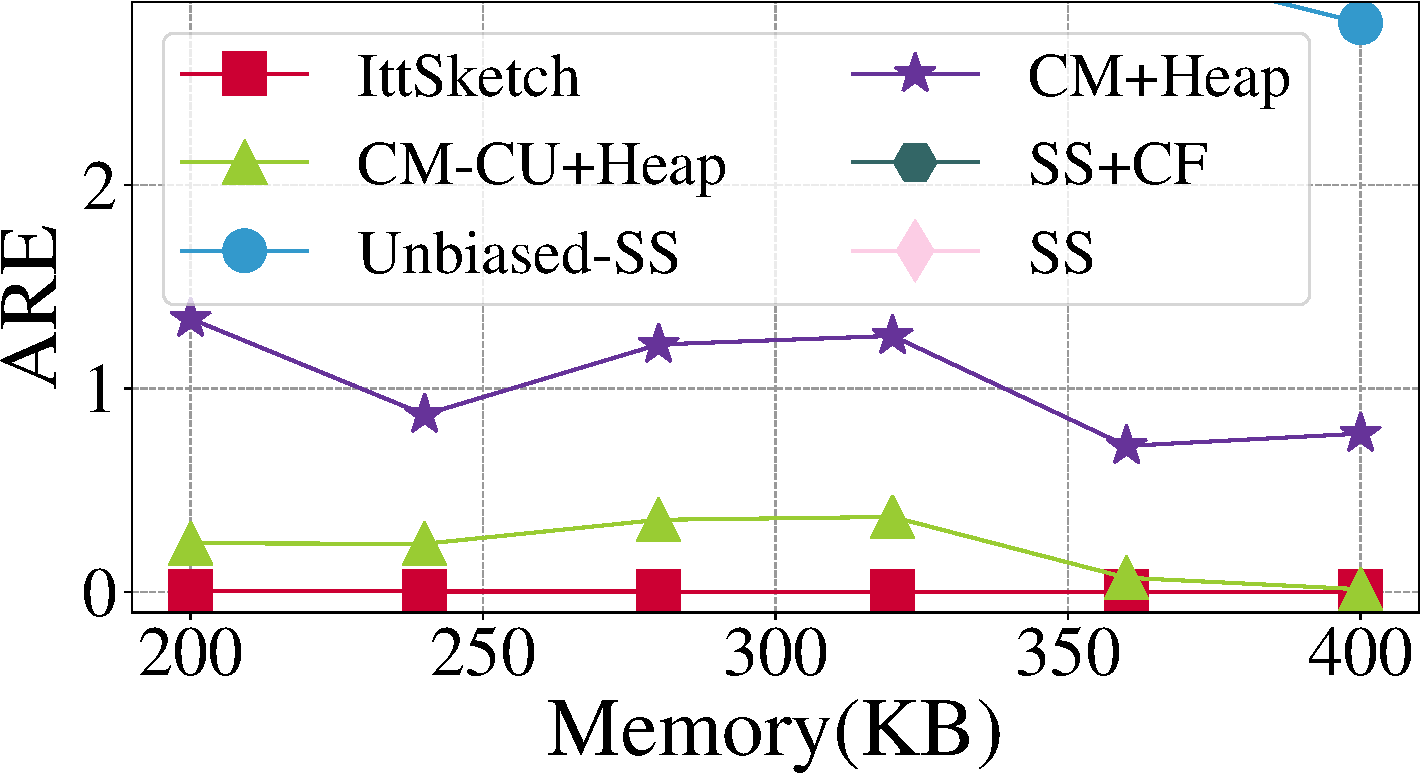
\includegraphics[width=0.95\textwidth, ]{Figures/fre/fre_are/fre_syn_are-cropped.pdf}
		\end{center}
		}
		\postfig 
		\adjustfigs
		\prefigcaption
		\label{fre_are_syn}
		\postfigcaption
		\end{minipage}
	}
	%
	\subfigure[IP trace]{
		\begin{minipage}[t]{0.23\textwidth}{
		\prefig
		\begin{center}
		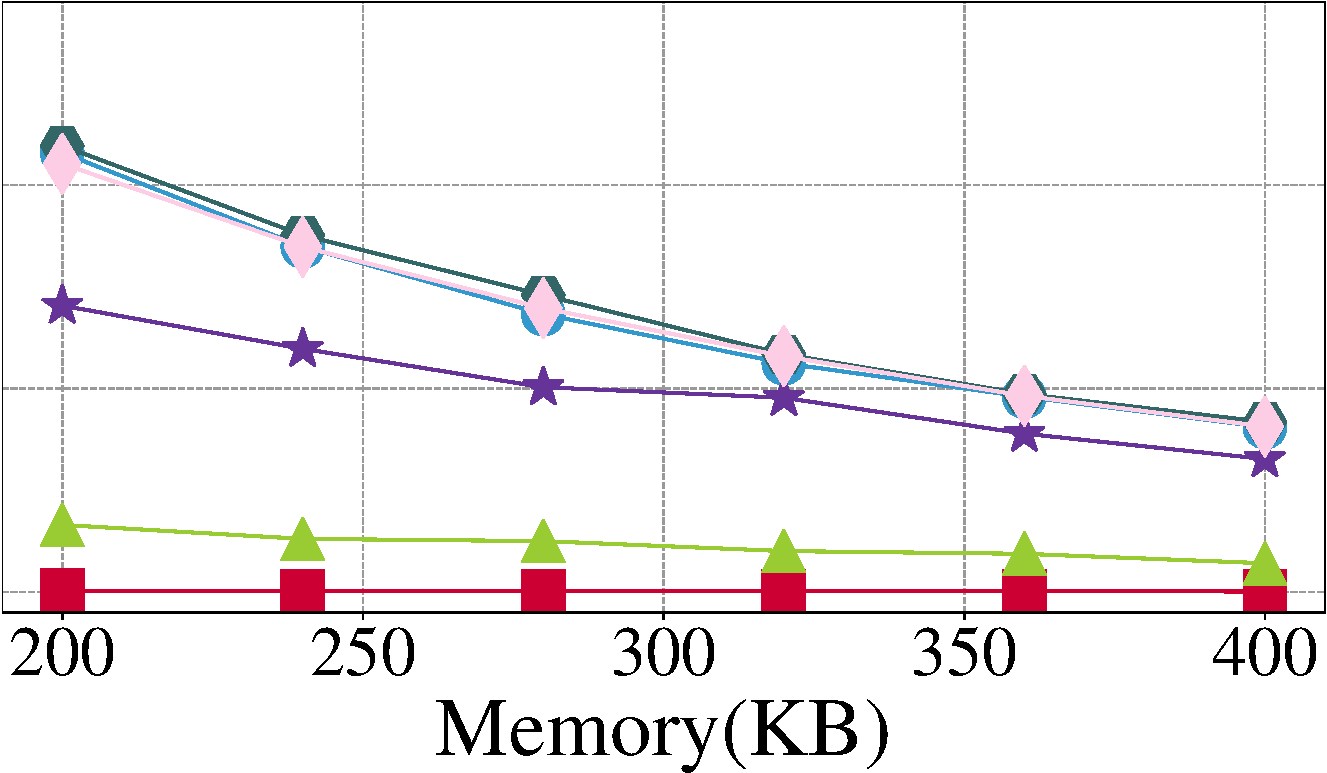
\includegraphics[width=0.95\textwidth, ]{Figures/fre/fre_are/fre_ip_are-cropped.pdf}
		\end{center}
		}
		\postfig
		\adjustfigs
		\prefigcaption
		\label{fre_are_ip}
		\postfigcaption
		\end{minipage}
	}
	%
	\subfigure[Web page]{
		\begin{minipage}[t]{0.23\textwidth}{
		\prefig
		\begin{center}		
		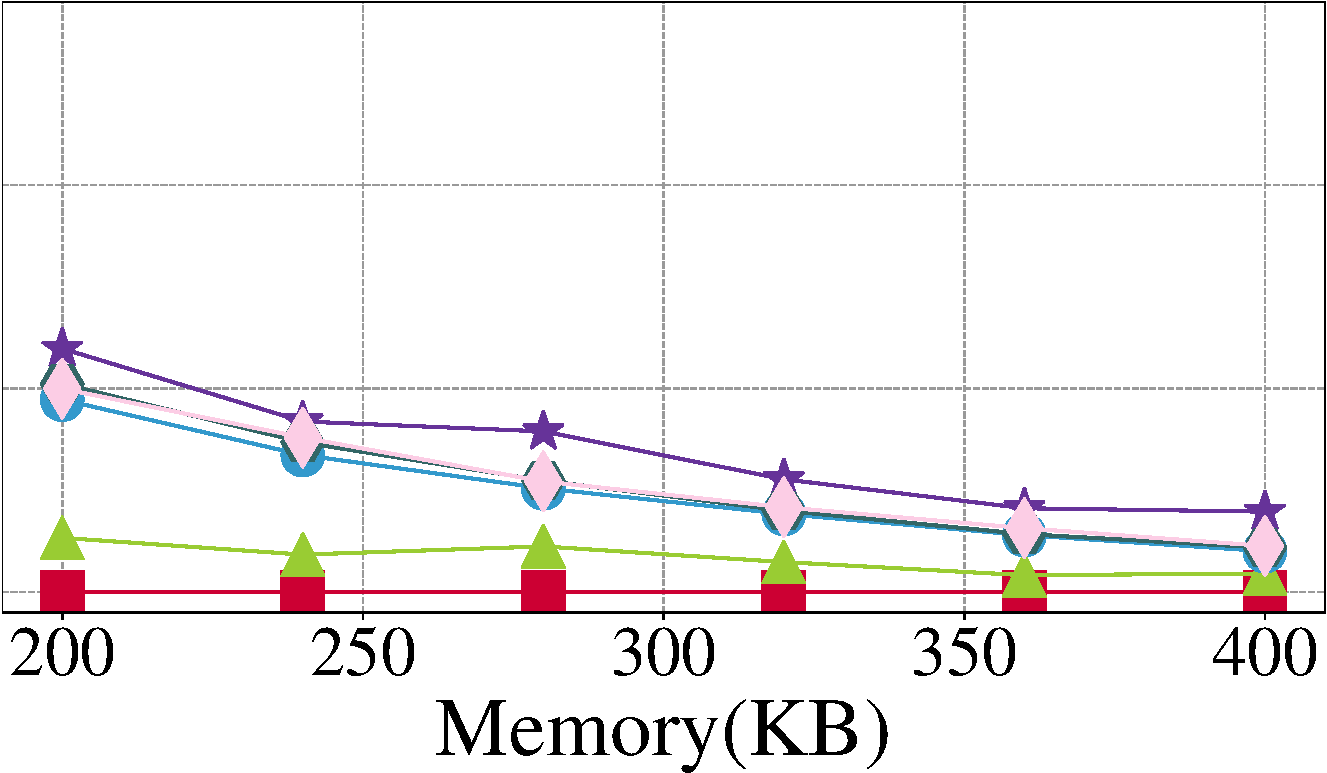
\includegraphics[width=0.95\textwidth, ]{Figures/fre/fre_are/fre_web_are-cropped.pdf}
		\end{center}
		}
	    \postfig 
	    \adjustfigs
	    \prefigcaption
		\label{fre_are_web}
		\postfigcaption
		\end{minipage}
	}
	%
	\subfigure[Network dataset]{
		\begin{minipage}[t]{0.23\textwidth}{
		\prefig
		\begin{center}		
		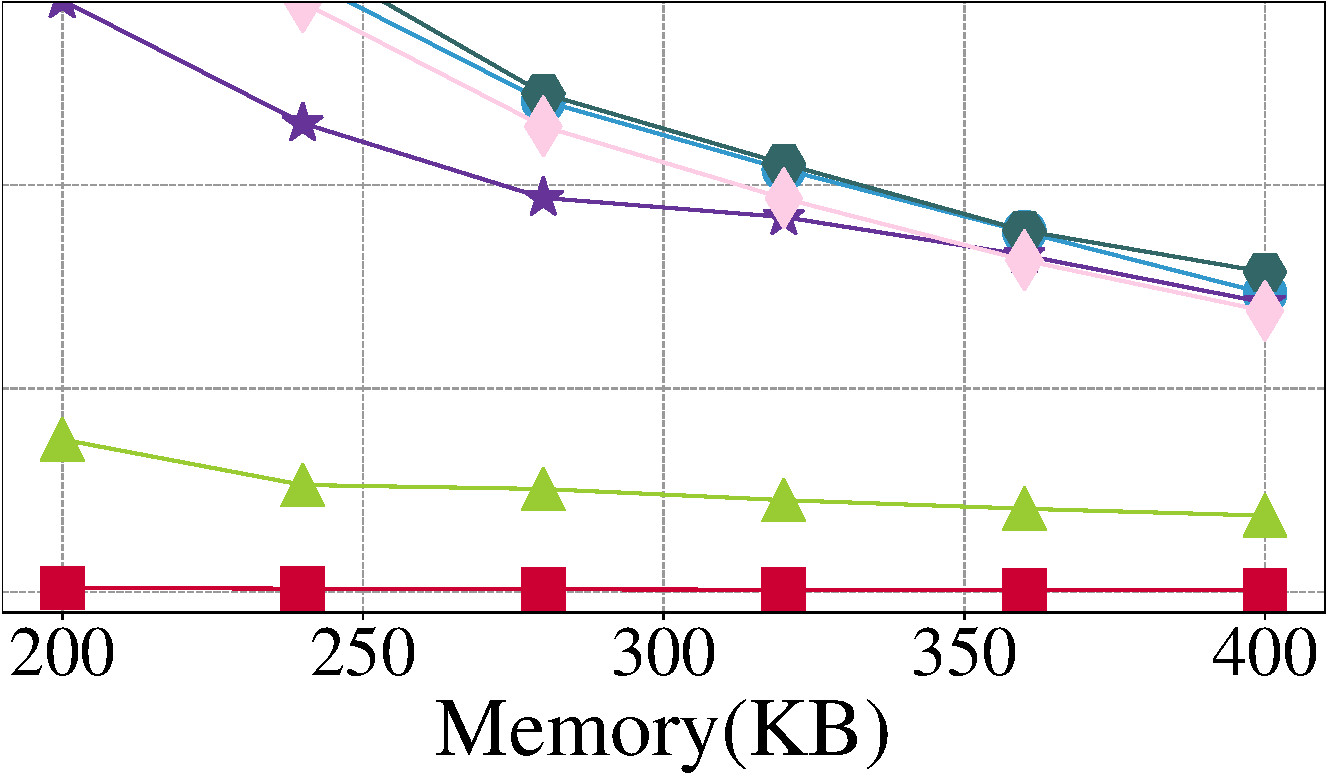
\includegraphics[width=0.95\textwidth, ]{Figures/fre/fre_are/fre_net_are-cropped.pdf}
		\end{center}
		}
		\postfig 
		\adjustfigs
		\prefigcaption
		\label{fre_are_net}
		\postfigcaption
		\end{minipage}
	}
	%
	\vvv \vvv
	\caption{ARE of finding \taskone.}
	\label{fre_are}
\end{figure*}
			
\begin{figure*}[!ht]
	\centering
	%
	\subfigure[Synthetic dataset]{
		\begin{minipage}[t]{0.255\textwidth}{
		\prefig
		\begin{center}
		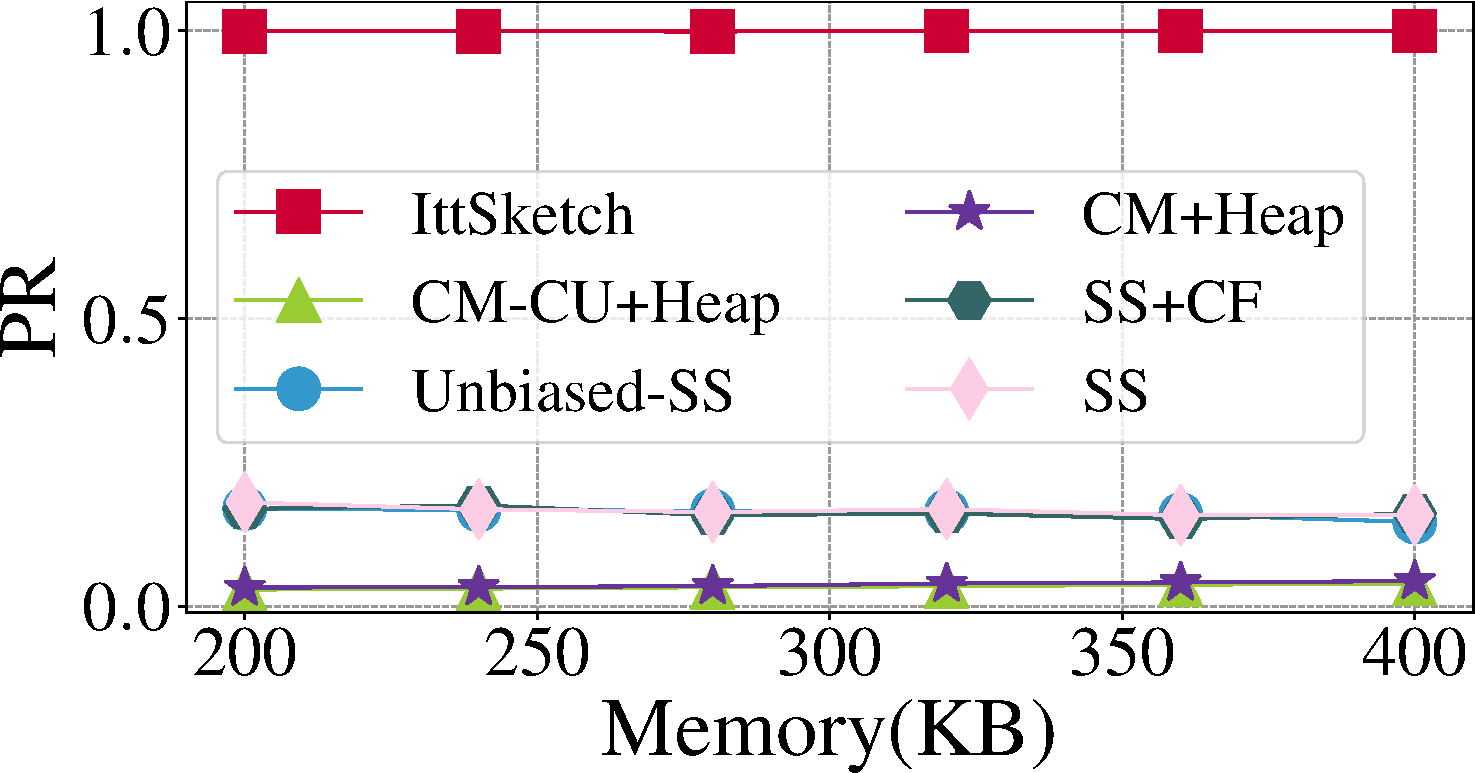
\includegraphics[width=0.95\textwidth, ]{Figures/fre/fre_pr/fre_syn_pr-cropped.pdf}
		\end{center}
		}
		\postfig 
		\adjustfigs
		\prefigcaption
		\label{fre_pr_syn}
		\postfigcaption
		\end{minipage}
	}
	%
	\subfigure[IP trace]{
		\begin{minipage}[t]{0.23\textwidth}{
		\prefig
		\begin{center}
		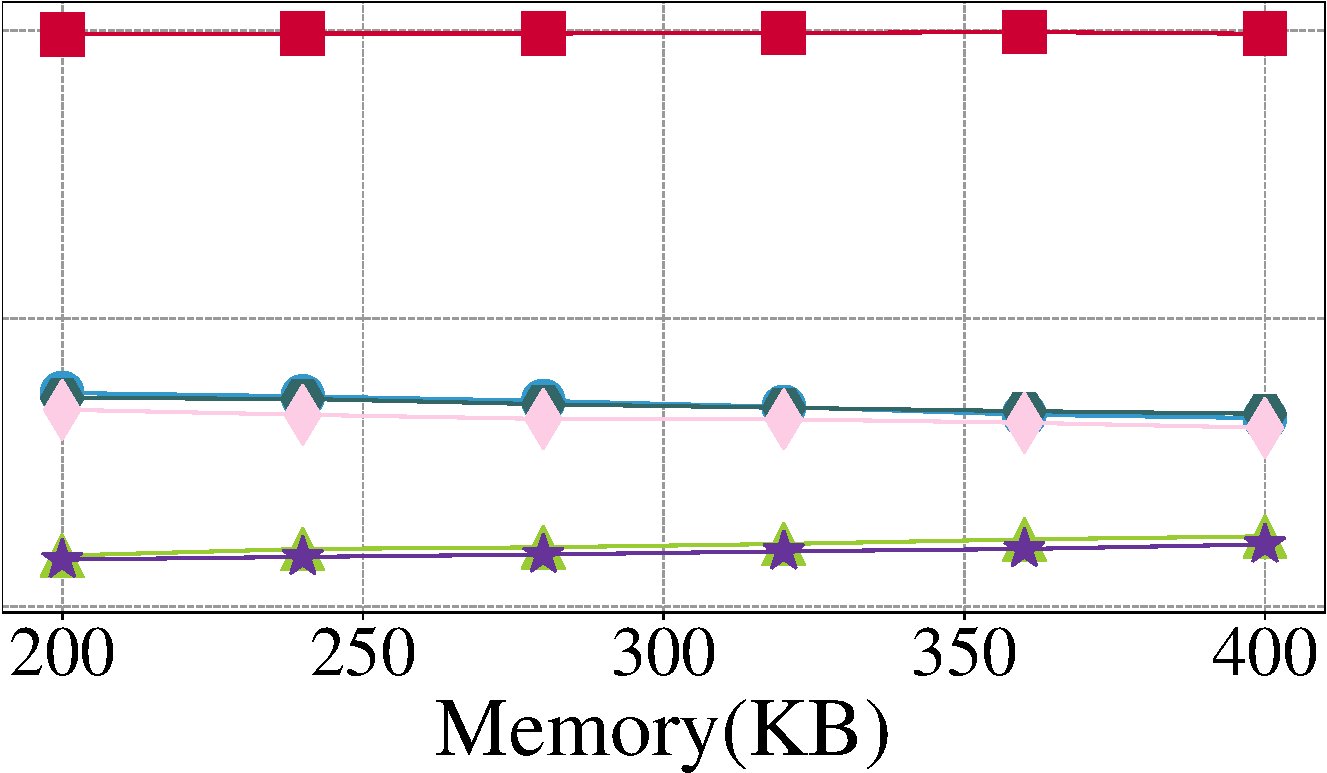
\includegraphics[width=0.95\textwidth, ]{Figures/fre/fre_pr/fre_ip_pr-cropped.pdf}
		\end{center}
		}
		\postfig
		\adjustfigs
		\prefigcaption
		\label{fre_pr_ip}
		\postfigcaption
		\end{minipage}
	}
	%
	\subfigure[Web page]{
		\begin{minipage}[t]{0.23\textwidth}{
		\prefig
		\begin{center}		
		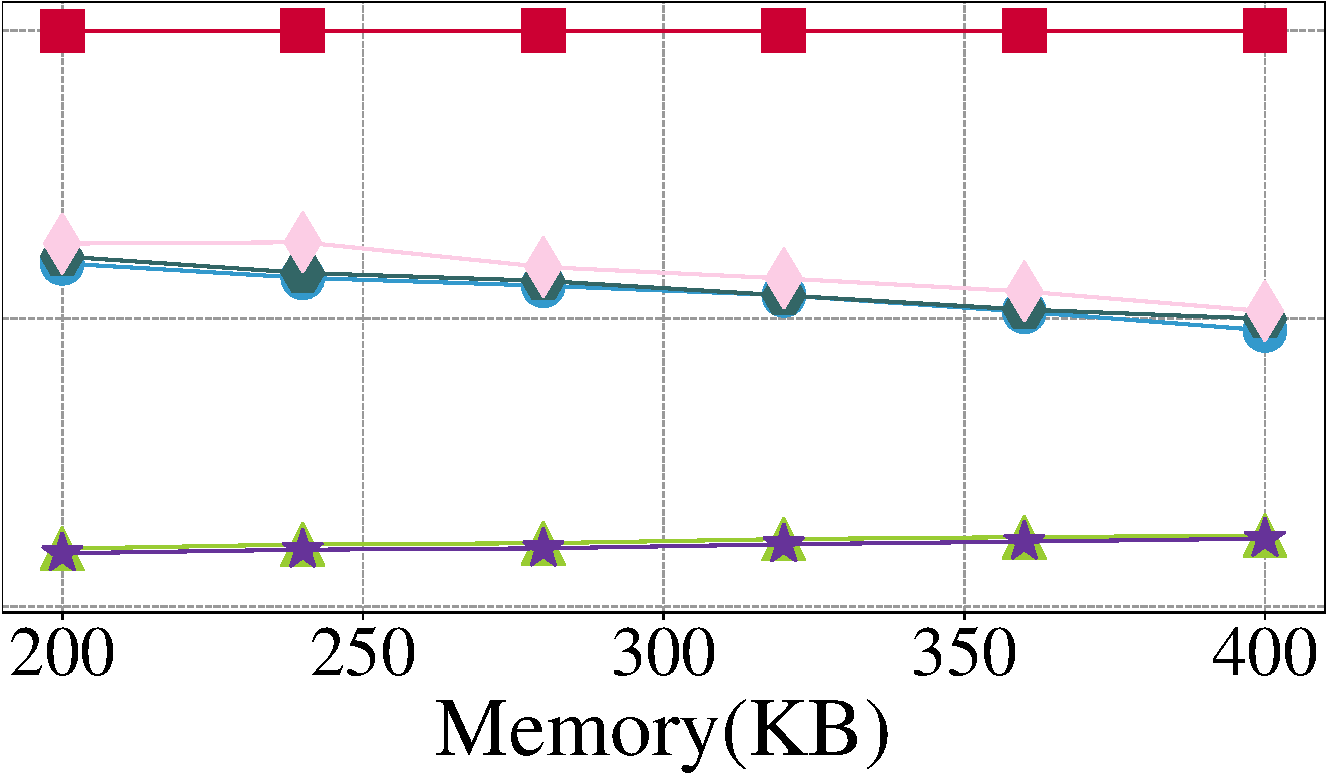
\includegraphics[width=0.95\textwidth, ]{Figures/fre/fre_pr/fre_web_pr-cropped.pdf}
		\end{center}
		}
		\postfig 
		\adjustfigs
		\prefigcaption
		\label{fre_pr_web}
		\postfigcaption
		\end{minipage}
	}
	%
	\subfigure[Network dataset]{
		\begin{minipage}[t]{0.23\textwidth}{
		\prefig
	    \begin{center}		
		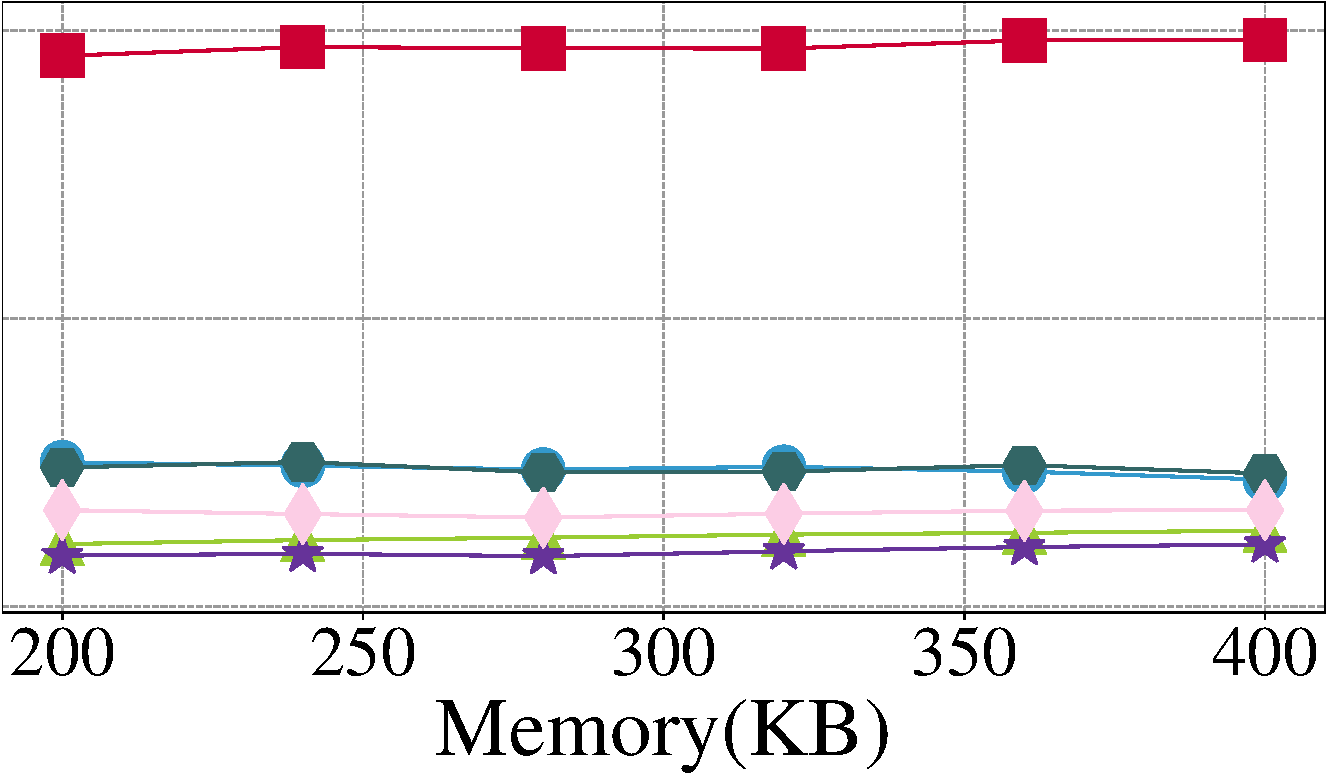
\includegraphics[width=0.95\textwidth, ]{Figures/fre/fre_pr/fre_net_pr-cropped.pdf}
		\end{center}
		}
		\postfig 
		\adjustfigs
		\prefigcaption
		\label{fre_pr_net}
		\postfigcaption
		\end{minipage}
	}
	%
	\vvv \vvv
    \caption{PR of finding \taskone.}
	\label{fre_pr}
\end{figure*}

\presub
\subsection{Experimental Setup} \postsub
\label{subsec:setup}
%
\noindent\textbf{Datasets:}

\noindent\textbf{1) IP Trace Dataset:}
The IP Trace Dataset are streams of anonymized IP traces collected in 2016 by CAIDA~\cite{caida}. Each item contains a source IP address ($4$ bytes) and a destination IP address ($4$ bytes){\color{reviewA} , 8 bytes in total.} {\color{reviewA} For this and the following three datasets, we assume that each item appears at most $2^{32}-1$ times.}

\noindent\textbf{2) Web Page Dataset:}
The Web page dataset is built from a collection of web pages, which were downloaded from the website~\cite{webdocs}.
Each item ($4$ bytes) represents the number of distinct terms in a web page.

\noindent\textbf{3) Synthetic Datasets:}
We generate 10 synthetic datasets which follow the Zipf~\cite{zipf} distribution by using Web Polygraph~\cite{webpoly}, an open source performance testing tool. Each dataset has 32 million items and the skewness of datasets varies from 0.3 to 3.0. The length of each item ID is $4$ bytes. 
In the following experiment, we use the dataset with skewness of 1.5 as synthetic dataset.

\noindent\textbf{4) Network Dataset:}
%This is a temporal network of interactions on the stack exchange web site \cite{net_dat}. Each item consists of three values $u,v,t$, which means user $u$ answered user $v'$s question at time t. We regard $u$ as an item ID and $t$ as its timestamp.
The network dataset contains users' posting history on the stack exchange website~\cite{net_dat}. Each item has three values $u,v,t$, that mean user $u$ answered user $v$'s question at time $t$. We use $u$ as the ID and $t$ as the time stamp of an item.

\noindent\textbf{Implementation:}
We have implemented \sketchname {} in C++.
The hash functions are implemented using the 32-bit Bob Hash (obtained from the open source website~\cite{bobhash}) with different initial seeds. The random function is implemented from the random library in C++. We produce the random number by using the random\_device from the <random> header file of the C++ standard library. All of the abbreviations used in the evaluation and their full name are shown in Table~\ref{abbr}.

\noindent\textbf{Computation Platform:}
We conducted all experiments on a machine with a 2-core processor (4 threads, 6th Gen Intel Core i7-6600U @2.60 GHz)
and 16 GB DRAM memory.
The processor has three levels of cache: one 128KB L1 cache, one 512KB L2 cache, and one 4MB L3 cache. 

\noindent\textbf{Metrics:}
\label{subsec:eva:metric}

%We use the following metrics (including accuracy metrics and insertion speed) to evaluate the performance of our algorithms. In experiment, we discover that after reading enough items (usually $1\sim2$ window sizes), the experiment result  will become stable. We measure the metrics in different window (after the first window), and compute the average value. We use the average value to represent the experiment result at given parameter setting. The error bar represents the minimal value and the maximum value.%

\noindent\textbf{1) Average Absolute Error (AAE):} $\frac{1}{|\mathbf{\Psi}|} \sum_{e_i \in \mathbf{\Psi}}|\iii_i-\widehat{\iii_i}| $,
where $\iii_i$ is the real interest of item $e_i$, $\widehat{\iii_i}$ is its estimated interest, and $\mathbf{\Psi}$ is the query set. 
Here, we query the dataset by querying every distinct item once in the sketch.

\noindent\textbf{2) Average Relative Error (ARE):} $\frac{1}{|\mathbf{\Psi}|} \sum_{e_i \in \mathbf{\Psi}}|\iii_i-\widehat{\iii_i}|/ \iii_i $,
where $\iii_i$ is the real interest of item $e_i$, $\widehat{\iii_i}$ is its estimated interest, and $\mathbf{\Psi}$ is the query set. 
Here, we query the dataset by querying each correct instance once in the sketch.

\noindent\textbf{3) Precision Rate (PR):}
Ratio of the number of correctly reported items to the number of reported items.

\noindent\textbf{4) Recall Rate (CR):}
Ratio of the number of correctly reported items to the number of correct items.

\noindent\textbf{5) Speed:}
Million operations (insertions) per second (Mops).
All the experiments about speed are repeated 10 times and the average speed is reported.

{\color{reviewD}
\noindent\textbf{6) Latency:}
Average process time needed by each item.
}

% Steve: a reviewer might want to see the standard deviation as well...

Let $d$ be the number of cells in each bucket. For our \sketchname{} in the following experiments, we set $d=8$.

\begin{table}
\vspace{-0.05in}
\caption{Abbreviations in experiment}
\vspace{-0.1in}
\label{abbr}
\begin{tabular}{|c|l|}
\hline
Abbreviation&Full name\\
\hline
CM&Count-Min Sketch\cite{cmsketch}\\
\hline
FR&Flow\cite{flowradar}\\
\hline
SS&SpaceSaving\cite{spacesaving}\\
\hline
CF&Cold Filter\cite{coldfilter}\\
\hline
OLF&One-level Filtering\cite{superspreader}\\  
\hline
TLF&Two-level Filtering\cite{superspreader}\\
\hline
SHF&Second Half First\\
\hline
IttSketch&The final version of \sketchname{} in \S \ref{sec:final}\\
\hline
\end{tabular}
\end{table}
\presub
\subsection{Evaluation on Finding \taskone} \postsub
\label{eva_one}

\noindent\textbf{Parameter Setting:}
%We compare three frameworks: \sketchname, \EHname and \Splittername. For each frameworks, we using CM Sketch, CM-CU Sketch and Count Sketch approaches.
%
%We compare 5 approaches: CM \sketchname, CM-CU \sketchname, Count \sketchname, \EHname {} and \Splittername.
%
We compare 6 algorithms: \sketchname, \freCM\cite{cmsketch}, \freCU\cite{cusketch}, \freCF\cite{coldfilter}, \freSS\cite{spacesaving}, and \freunbia\cite{unbiasedsketch}.
For \freCM, \freCU{}, and \freCF, the parameters are set according to the recommendation of the authors.
In this experiment, we compare AAE, ARE, PR, CR, and insertion speed among the 6 algorithms.
The size of memory used ranges from 200KB to 400KB. We choose this range because: 1) \sketchname{} has performed well enough in this range and 2) relying on little memory will expose the difference between the algorithms.
			
\noindent\textbf{ARE (Figure~\ref{fre_are_syn}-\ref{fre_are_net}):}
We find that, on three real-world datasets, the ARE of \sketchname{} is around 3207 times, 708 times, 2735 times, 2707 times, and 2576 times lower than \freCM, \freCU, \freCF, \freSS{}, and \freunbia{}, respectively. On the synthetic dataset, the ARE of \sketchname{} is around 416 times, 74 times, 1851 times, 1866 times, and 1820 times lower than \freCM, \freCU, \freCF, \freSS{}, and \freunbia{}, respectively.
			
\noindent\textbf{PR (Figure~\ref{fre_pr_syn}-\ref{fre_pr_net}):}
We find that on three real-world datasets, the PR of \sketchname{} is around 11.2 times, 9.9 times, 2.8 times, 3.4 times, and 2.7 times higher than \freCM, \freCU, \freCF, \freSS{}, and \freunbia{} respectively. On the synthetic dataset, the PR of \sketchname{} is around 30.3 times, 33.8 times, 5.9 times, 5.5 times, and 5.8 times higher than \freCM, \freCU, \freCF, \freSS{}, and \freunbia{}, respectively.
	
\begin{figure*}[!ht]
	\centering
	%
	\subfigure[Synthetic dataset]{
		\begin{minipage}[t]{0.252\textwidth}{
		\prefig
		\begin{center}
		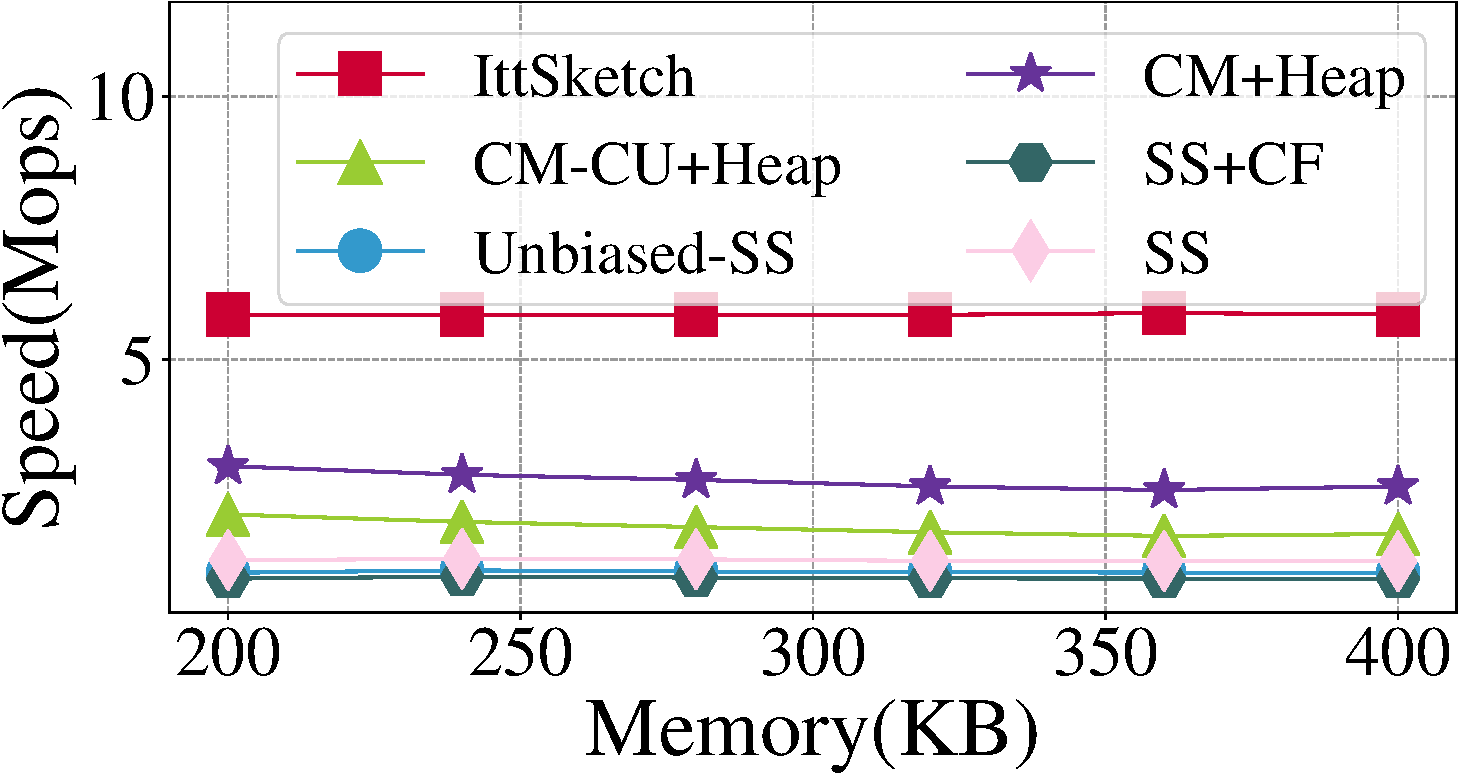
\includegraphics[width=0.95\textwidth, ]{Figures/fre/fre_speed/fre_syn_speed-cropped.pdf}
		\end{center}
		}
		\postfig 
		\adjustfigs
		\prefigcaption
		\label{fre_speed_syn}
		\postfigcaption
		\end{minipage}
	}
	%
	\subfigure[IP trace]{
		\begin{minipage}[t]{0.23\textwidth}{
		\prefig
		\begin{center}
		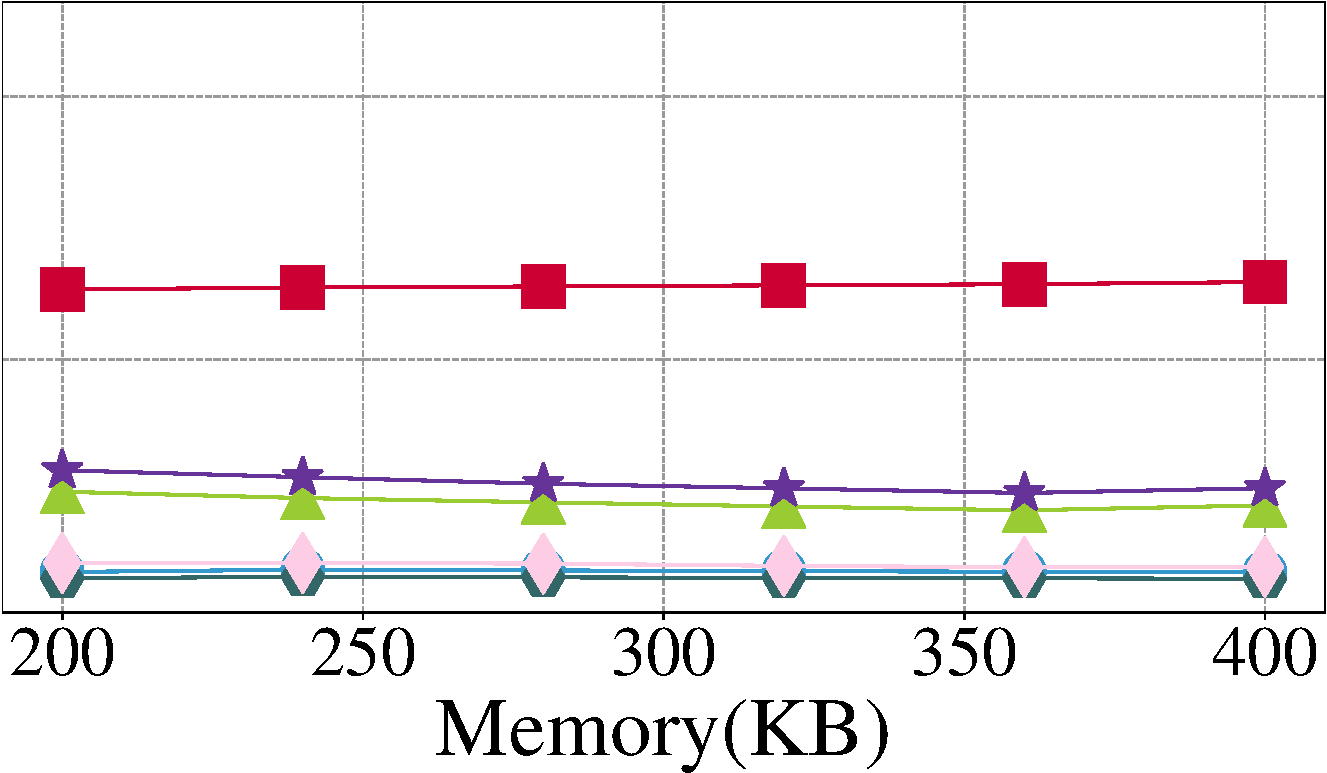
\includegraphics[width=0.95\textwidth, ]{Figures/fre/fre_speed/fre_ip_speed-cropped.pdf}
		\end{center}
		}
		\postfig
		\adjustfigs
		\prefigcaption
		\label{fre_speed_ip}\postfigcaption
		\end{minipage}
	}
	%
	\subfigure[Web page]{
		\begin{minipage}[t]{0.23\textwidth}{
		\prefig
		\begin{center}		
		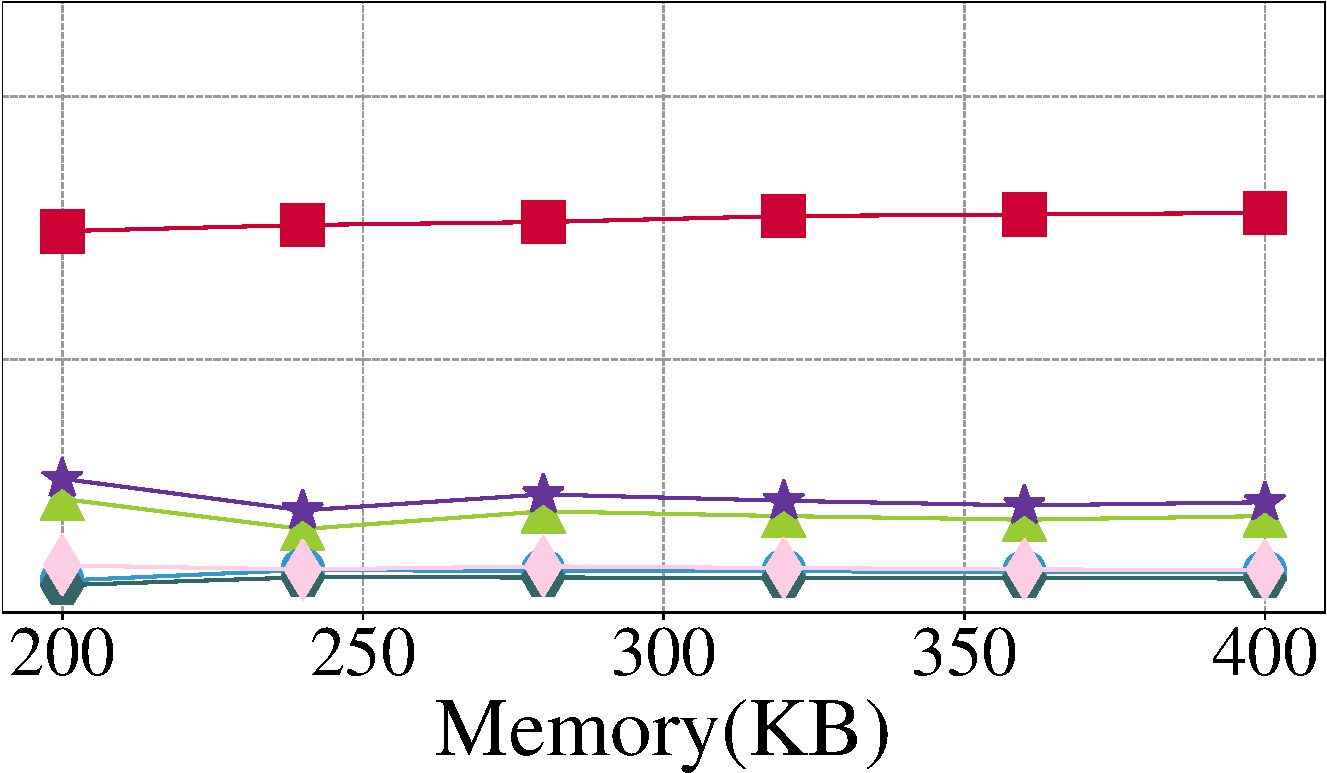
\includegraphics[width=0.95\textwidth, ]{Figures/fre/fre_speed/fre_web_speed-cropped.pdf}
		\end{center}
		}
		\postfig 
		\adjustfigs
		\prefigcaption
		\label{fre_speed_web}
		\postfigcaption
		\end{minipage}
	}
	%
	\subfigure[Network dataset]{
		\begin{minipage}[t]{0.23\textwidth}{
		\prefig
		\begin{center}		
		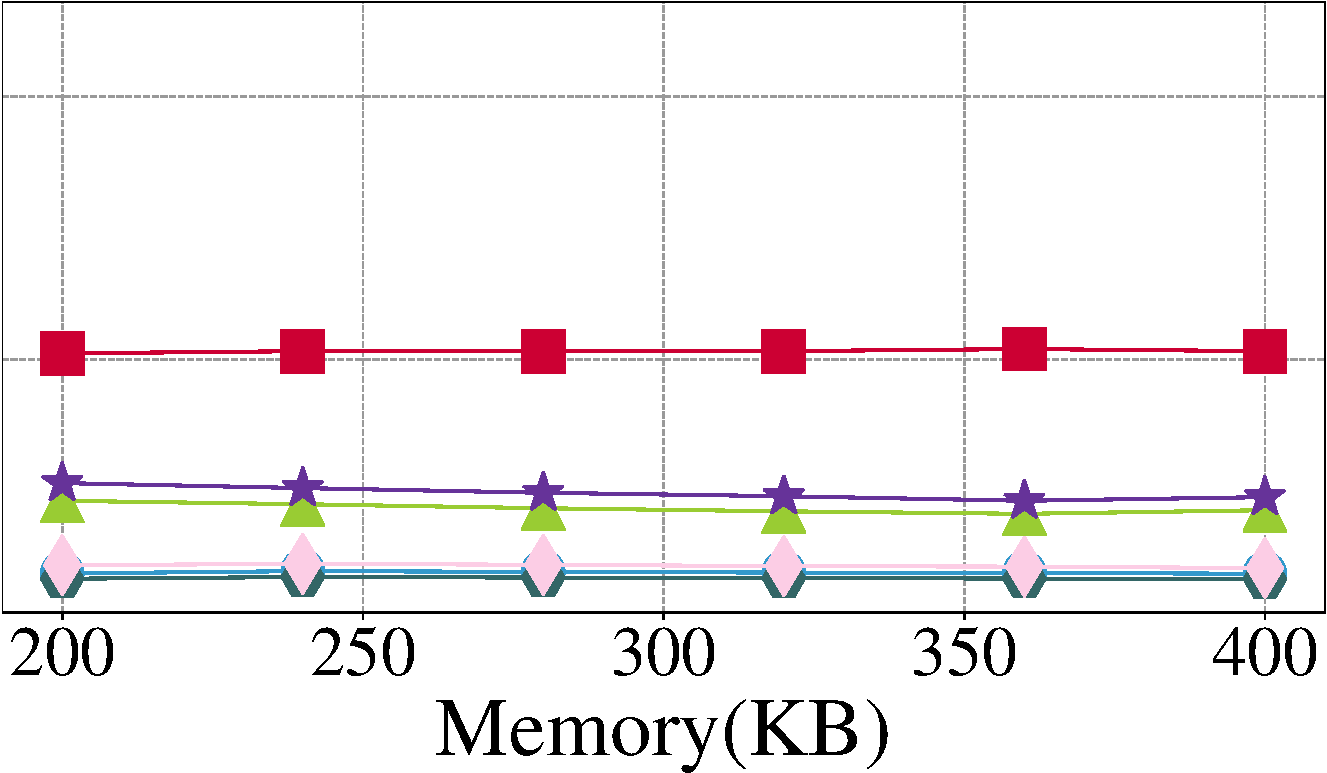
\includegraphics[width=0.95\textwidth, ]{Figures/fre/fre_speed/fre_net_speed-cropped.pdf}
		\end{center}
		}
		\postfig 
		\adjustfigs
		\prefigcaption
		\label{fre_speed_net}
		\postfigcaption
		\end{minipage}
	}
	\vvv \vvv
	\caption{Speed of finding \taskone.}
	\label{fre_speed}
\end{figure*}		
			
\noindent\textbf{Speed (Figure~\ref{fre_speed_syn}-\ref{fre_speed_net}):}
We find that, on three real-world datasets and one synthetic dataset, the insertion speed of \sketchname{} is around 2.2 times, 2.7 times, 7.7 times, 5.48 times, and 6.7 times faster than \freCM, \freCU, \freCF, \freSS{}, and \freunbia{}, respectively.


\noindent\textbf{AAE (Figure~\ref{fre_aae_syn}-\ref{fre_aae_net}) in Appendix \ref{app:fig}:}
We find that, on three real-world datasets, the AAE of \sketchname{} is around 7309 times, 995 times, 3860 times, 3701 times, and 3549 times lower than \freCM, \freCU, \freCF, \freSS{}, and \freunbia{}, respectively. Besides, on the synthetic dataset, the AAE of \sketchname{} is around 2278 times, 80 times, 3247 times, 3278 times, and 3205 times lower than \freCM, \freCU, \freCF, \freSS{}, and \freunbia{}, respectively. 

\begin{figure*}[!ht]
	\centering
	%
	\subfigure[Synthetic dataset]{
		\begin{minipage}[t]{0.255\textwidth}{
		\prefig
		\begin{center}
		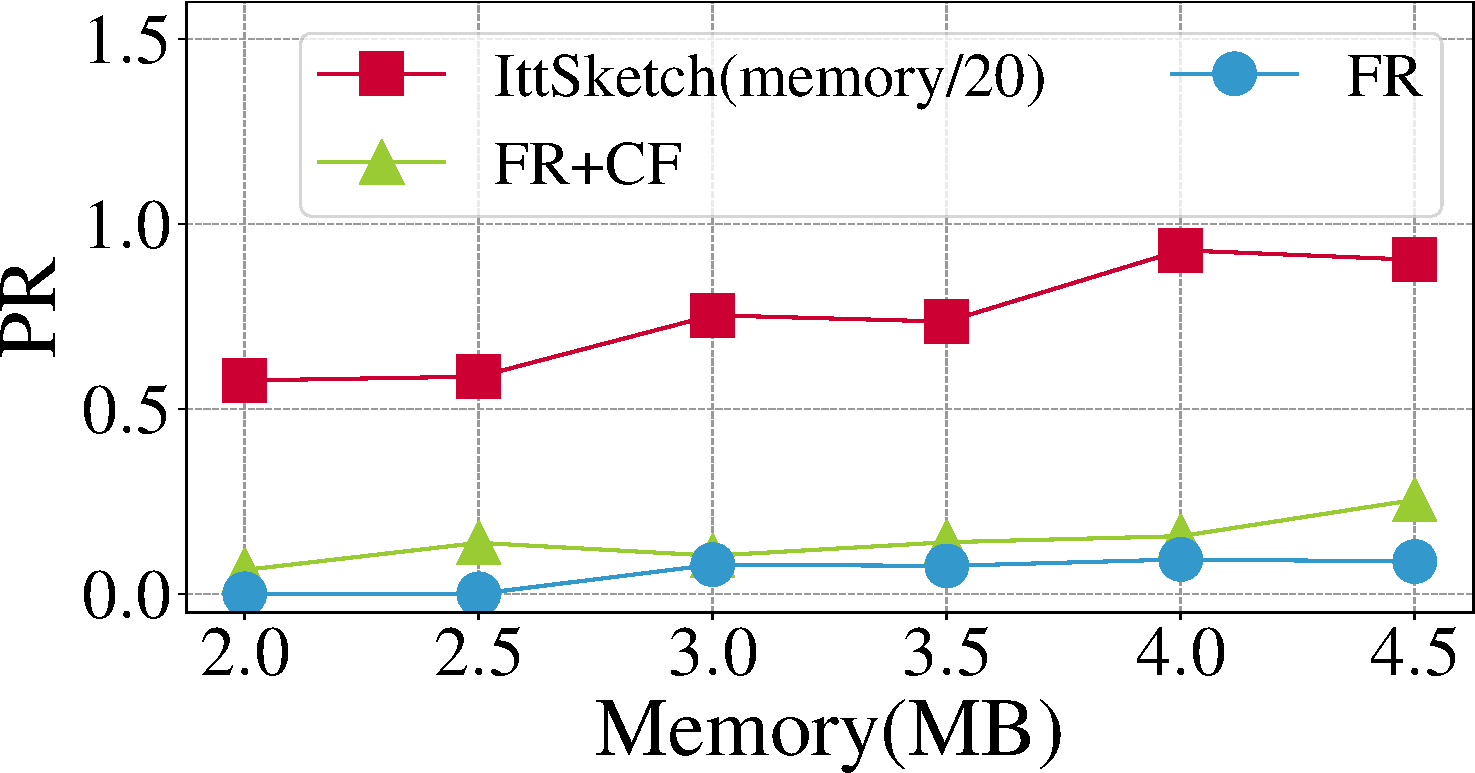
\includegraphics[width=0.95\textwidth, ]{Figures/cha/cha_pr/cha_syn_pr-cropped.pdf}
		\end{center}
		}
		\postfig 
		\adjustfigs
		\prefigcaption
		\label{cha_pr_syn}
		\postfigcaption
		\end{minipage}
	}
	%
	\subfigure[IP trace]{
		\begin{minipage}[t]{0.23\textwidth}{
		\prefig
		\begin{center}
		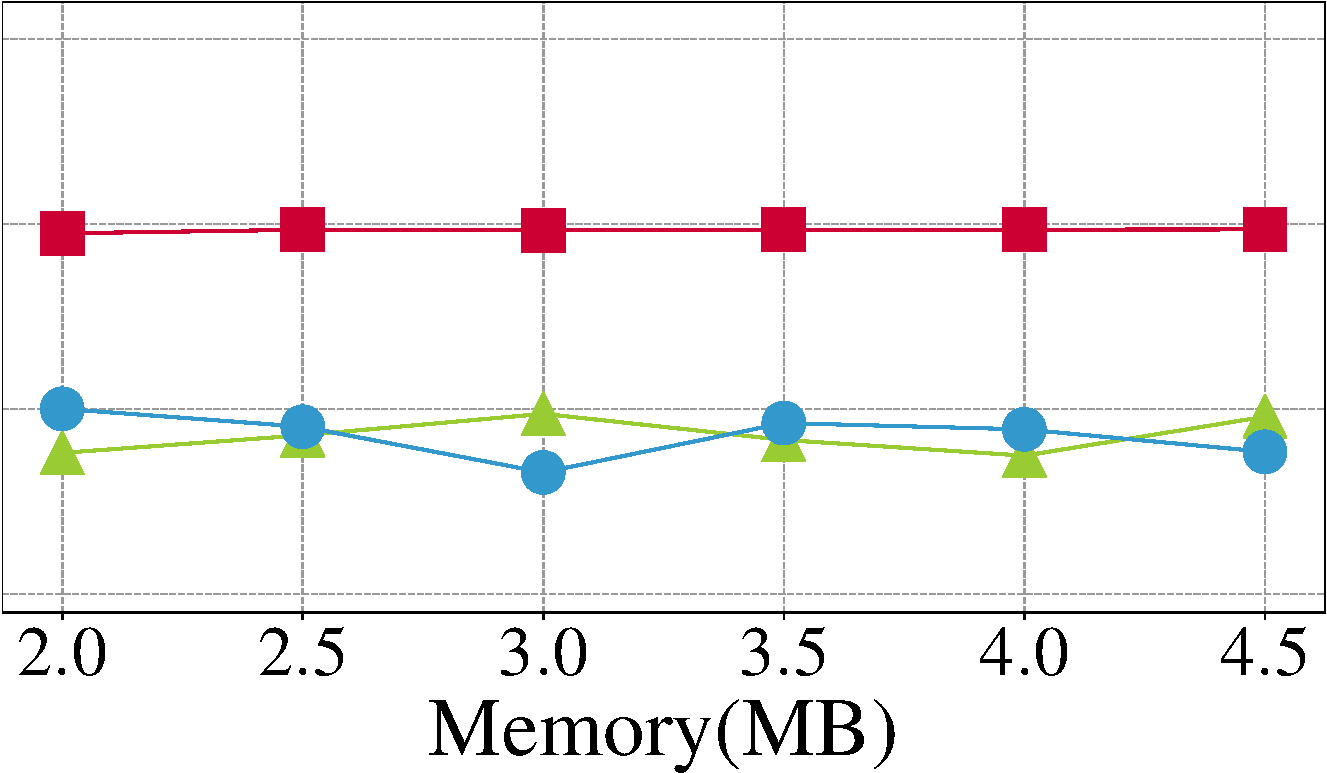
\includegraphics[width=0.95\textwidth, ]{Figures/cha/cha_pr/cha_ip_pr-cropped.pdf}
		\end{center}
		}
		\postfig
		\adjustfigs
		\prefigcaption
		\label{cha_pr_ip}
		\postfigcaption
		\end{minipage}
	}
	%
	\subfigure[Web page]{
		\begin{minipage}[t]{0.23\textwidth}{
		\prefig
		\begin{center}		
		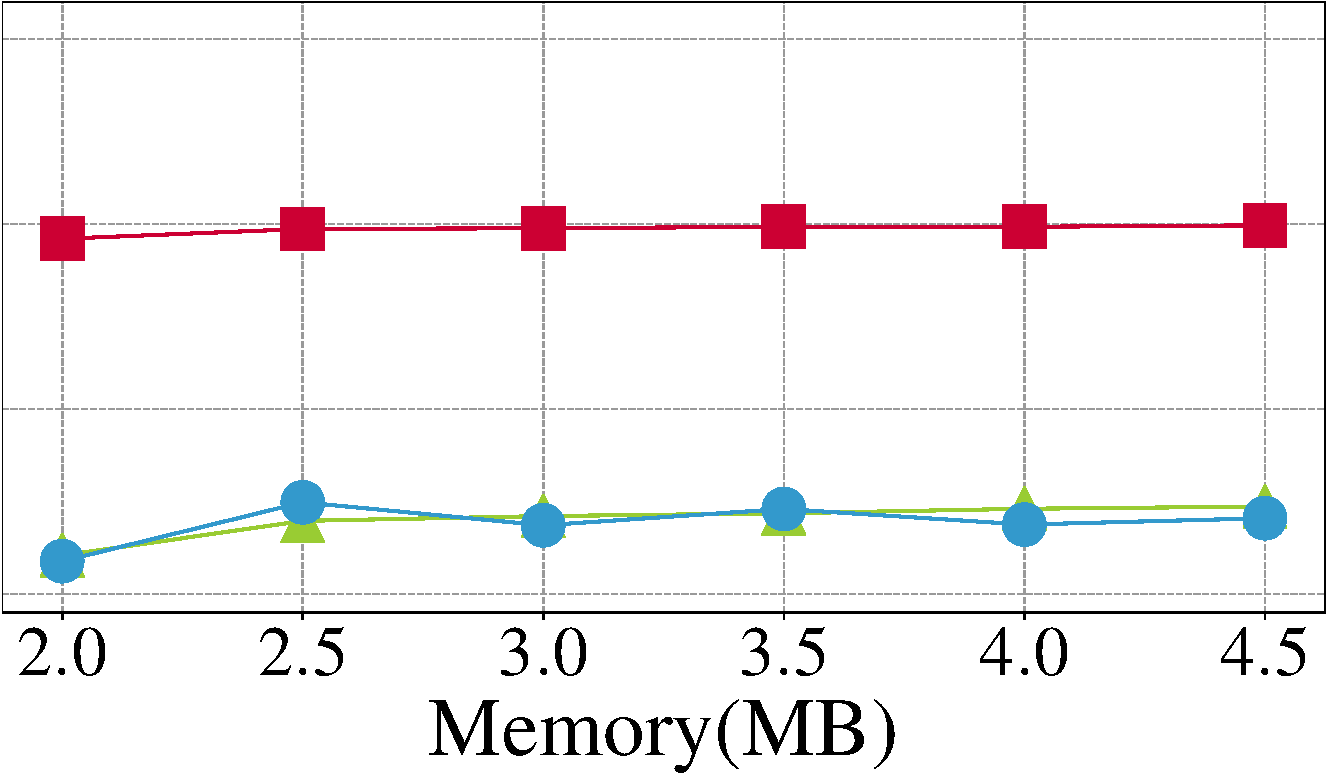
\includegraphics[width=0.95\textwidth, ]{Figures/cha/cha_pr/cha_web_pr-cropped.pdf}
		\end{center}
		}
		\postfig 
		\adjustfigs
		\prefigcaption
		\label{cha_pr_web}
		\postfigcaption
		\end{minipage}
	}
	%
	\subfigure[Network dataset]{
		\begin{minipage}[t]{0.23\textwidth}{
		\prefig
	    \begin{center}		
		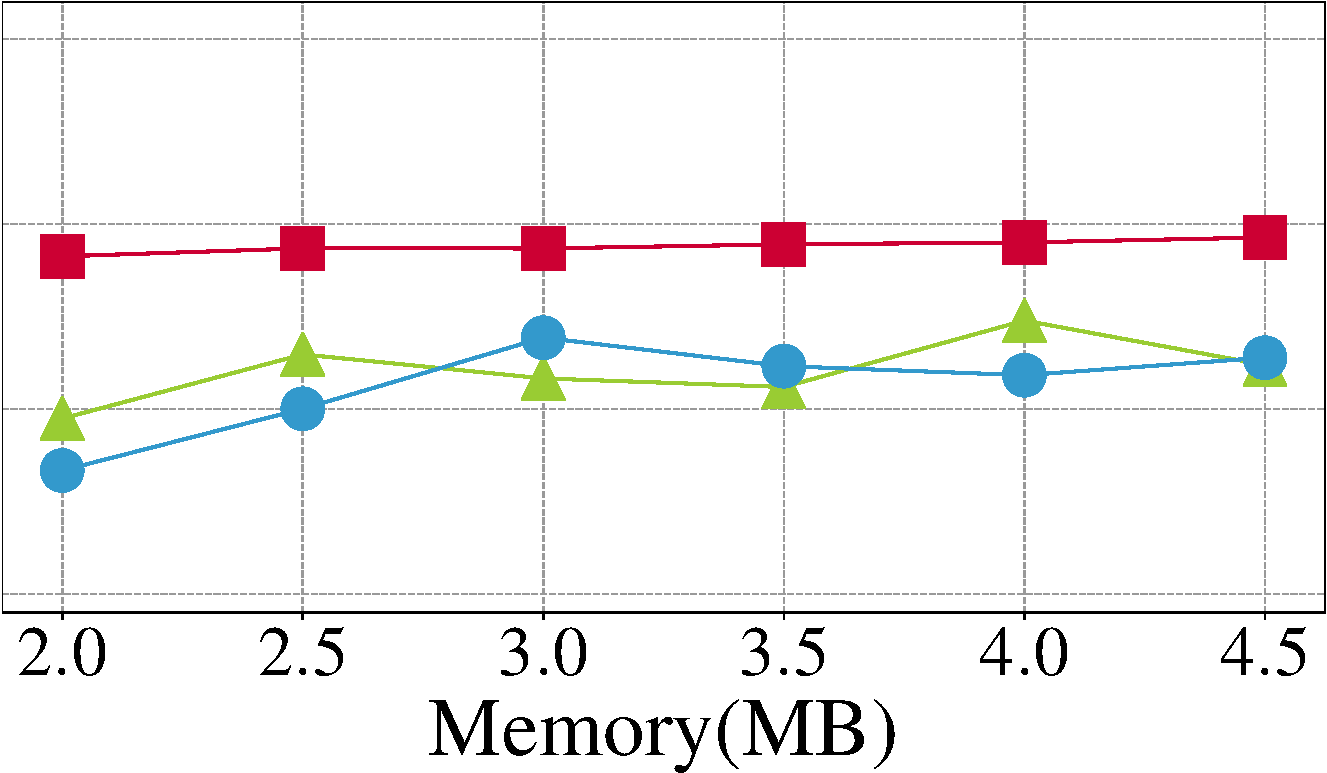
\includegraphics[width=0.95\textwidth, ]{Figures/cha/cha_pr/cha_net_pr-cropped.pdf}
		\end{center}
		}
		\postfig 
		\adjustfigs
		\prefigcaption
		\label{cha_pr_net}
		\postfigcaption
		\end{minipage}
	}
	%
	\vvv \vvv
    \caption{PR of finding \taskfour.}
	\label{cha_pr}
\end{figure*}

\begin{figure*}[!ht]
	\centering
	%
	\subfigure[Synthetic dataset]{
		\begin{minipage}[t]{0.24546\textwidth}{
		\prefig
		\begin{center}
		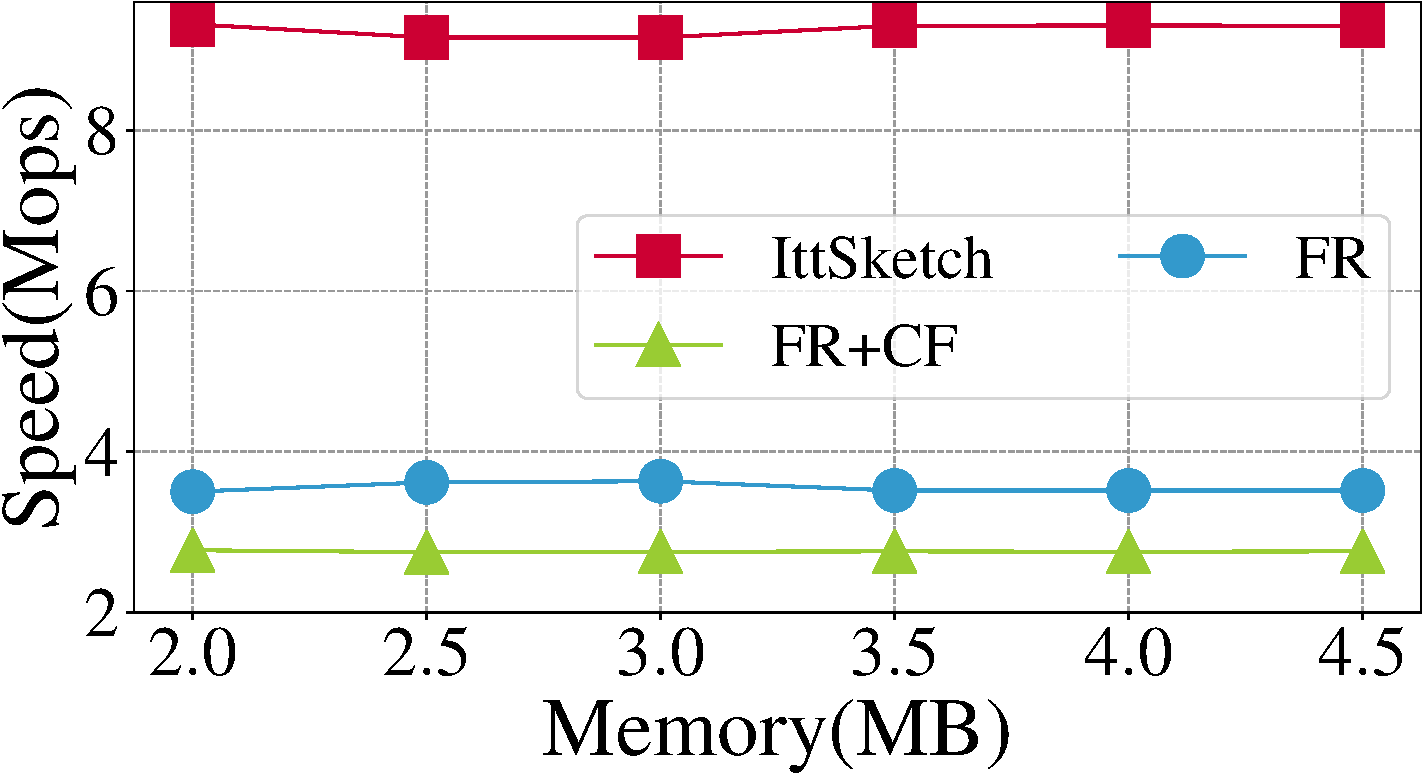
\includegraphics[width=0.95\textwidth, ]{Figures/cha/cha_speed/cha_syn_speed-cropped.pdf}
		\end{center}
		}
		\postfig 
		\adjustfigs
		\prefigcaption
		\label{cha_speed_syn}
		\postfigcaption
		\end{minipage}
	}
	%
	\subfigure[IP trace]{
		\begin{minipage}[t]{0.23\textwidth}{
		\prefig
		\begin{center}
		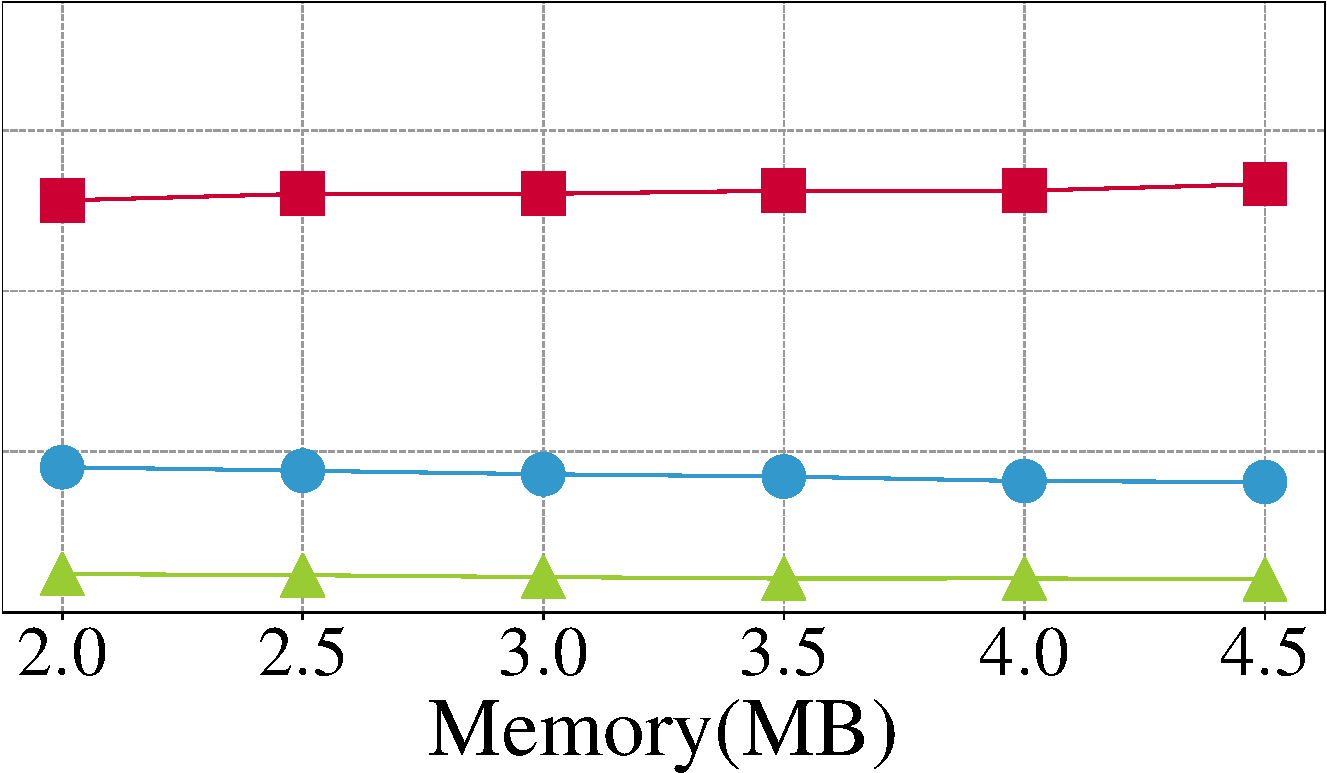
\includegraphics[width=0.95\textwidth, ]{Figures/cha/cha_speed/cha_ip_speed-cropped.pdf}
		\end{center}
		}
		\postfig
		\adjustfigs
		\prefigcaption
		\label{cha_speed_ip}
		\postfigcaption
		\end{minipage}
	}
	%
	\subfigure[Web page]{
		\begin{minipage}[t]{0.23\textwidth}{
		\prefig
		\begin{center}		
		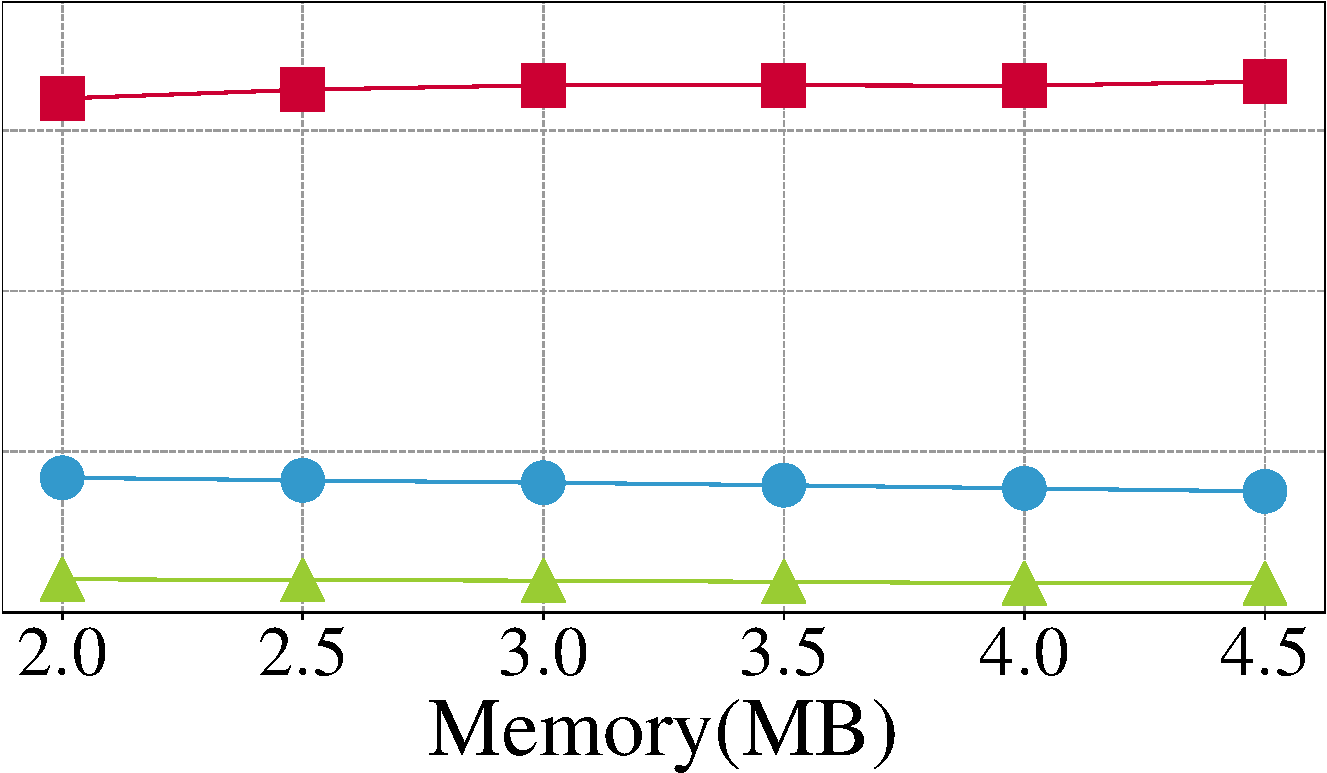
\includegraphics[width=0.95\textwidth, ]{Figures/cha/cha_speed/cha_web_speed-cropped.pdf}
		\end{center}
		}
		\postfig 
		\adjustfigs
		\prefigcaption
		\label{cha_speed_web}
		\postfigcaption
		\end{minipage}
	}
	%
	\subfigure[Network dataset]{
		\begin{minipage}[t]{0.23\textwidth}{
		\prefig
		\begin{center}		
		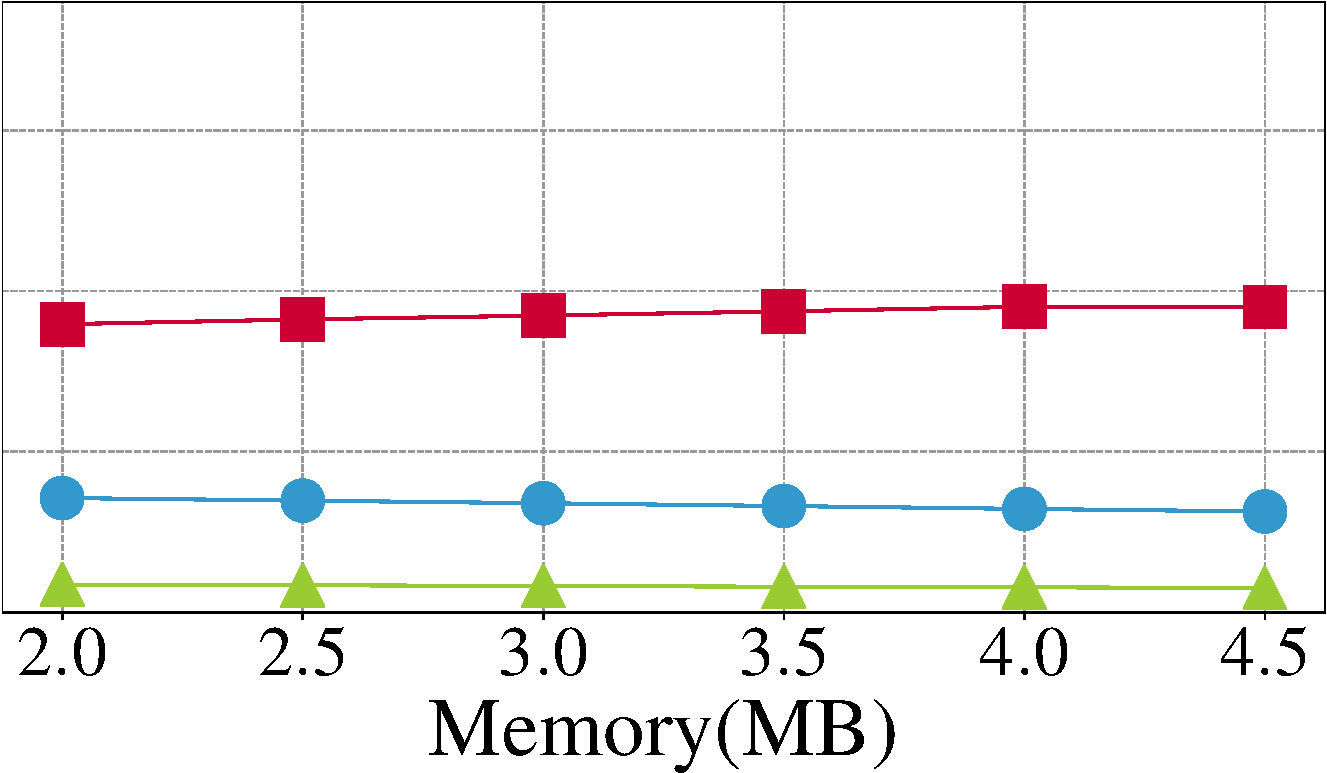
\includegraphics[width=0.95\textwidth, ]{Figures/cha/cha_speed/cha_net_speed-cropped.pdf}
		\end{center}
		}
		\postfig 
		\adjustfigs
		\prefigcaption
		\label{cha_speed_net}
		\postfigcaption
		\end{minipage}
	}
	%
	\vvv \vvv
    \caption{Speed of finding \taskfour.}
	\label{cha_speed}
\end{figure*}

\noindent\textbf{CR (Figure~\ref{fre_cr_syn}-\ref{fre_cr_net}) in Appendix \ref{app:fig}:}
We find that, on three real-world datasets, the CR of \sketchname{} is around 5.6 times, 5 times, 1.7 times, 2 times, and 1.6 times higher than \freCM, \freCU, \freCF, \freSS{}, and \freunbia{}, respectively. 
On the synthetic dataset, the CR of \sketchname{} is around 17 times, 18 times, 5 times, 4.7 times, and 5.3 times higher than \freCM, \freCU, \freCF, \freSS{}, and \freunbia{}, respectively.


\noindent\textbf{Summary:}
%
1) \sketchname{} can achieve high accuracy with limited memory. The ARE of \sketchname{} is lower than 0.01 when the memory is set to 200KB, while the ARE of the other algorithms is often higher than 1. As seen in the figures, the ARE of \freSS, \freCF{}, and \freunbia{} often exceed the range of the plots.

2) \sketchname{} can report more correct instances than other approaches. \sketchname{} often reports more than 99 percent of the correct instances, while the other approaches report less than 40 percent, because they often consume too much memory on the hash table or Stream-Summary.

3) \sketchname{} achieves higher precision in reported instances. The PR of \sketchname{} is often higher than 0.99, while the PR of other approaches is often less than 0.6 because they overestimate the results. 

4) The insertion speed of \sketchname{} is also faster than the other approaches for the same memory consumption on three real-world datasets and one synthetic dataset.
\begin{figure*}[!ht]
	\centering
	%
	\subfigure[IP trace1]{
		\begin{minipage}[t]{0.255\textwidth}{
		\prefig
		\begin{center}
		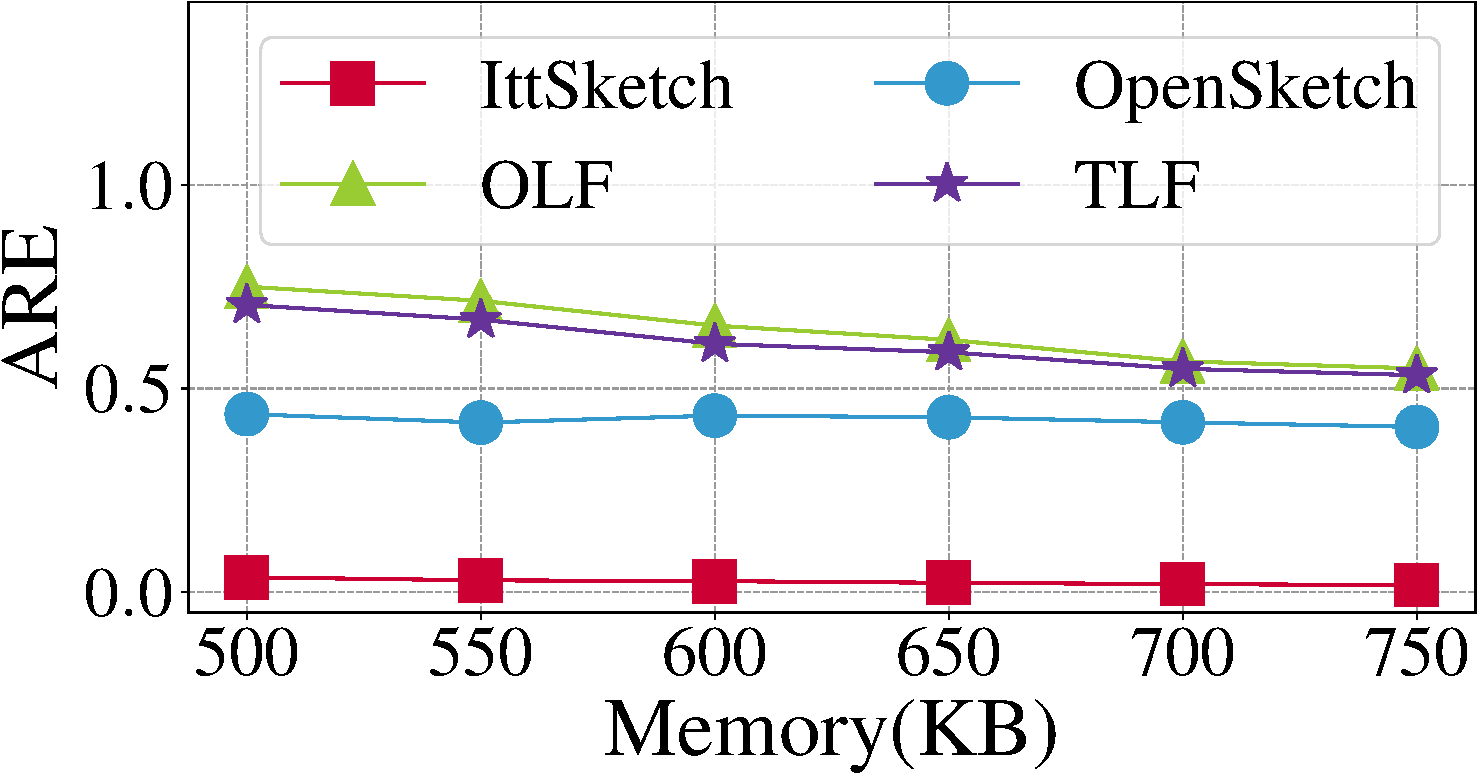
\includegraphics[width=0.95\textwidth, ]{Figures/sup/sup_are/_sup_ip_are.pdf}
		\end{center}
		}
		\postfig
		\adjustfigs
		\prefigcaption
		\label{sup_are_ip}
		\postfigcaption
		\end{minipage}
	}
	%
	\subfigure[IP trace2]{
		\begin{minipage}[t]{0.23\textwidth}{
		\prefig
		\begin{center}		
		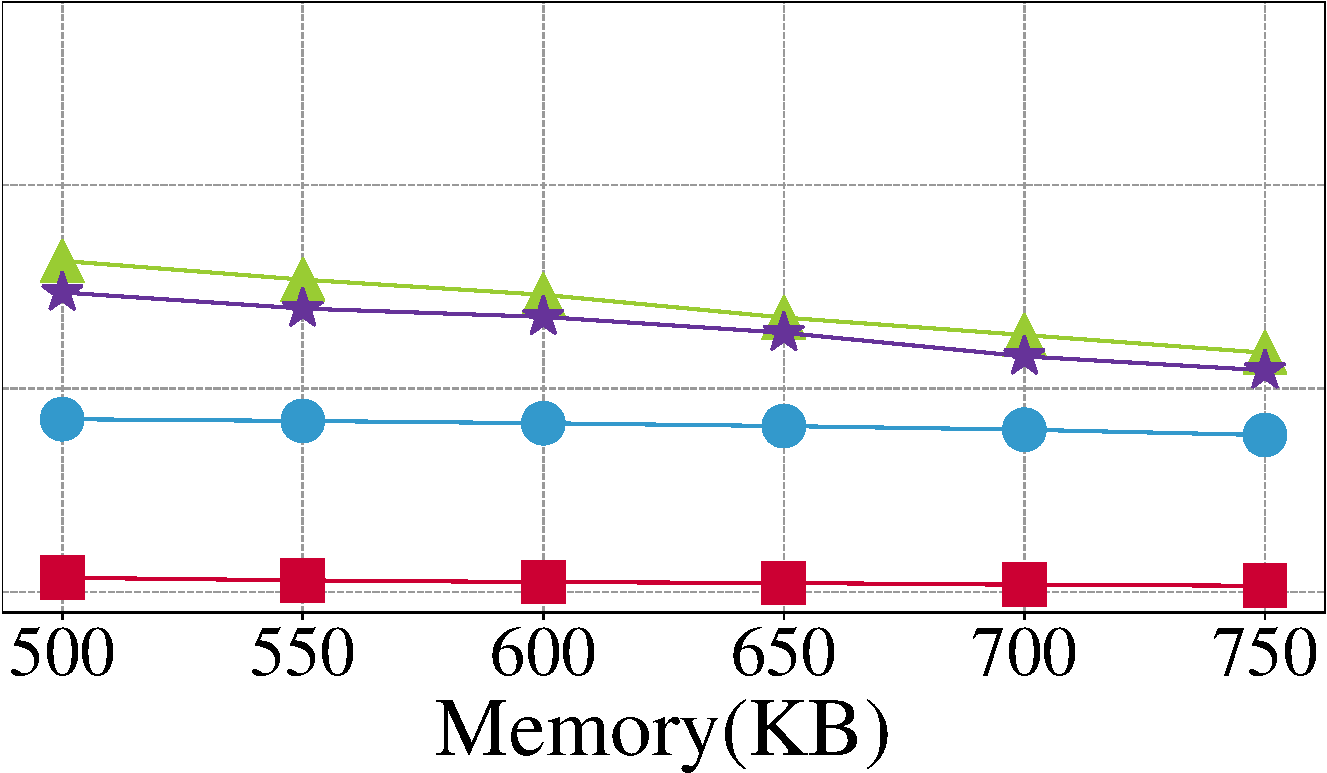
\includegraphics[width=0.95\textwidth, ]{Figures/sup/sup_are/_sup_ip4_are.pdf}
		\end{center}
		}
		\postfig 
		\adjustfigs
		\prefigcaption
		\label{sup_are_ip4}
		\postfigcaption
		\end{minipage}
	}
	%
	\subfigure[IP trace3]{
		\begin{minipage}[t]{0.23\textwidth}{
		\prefig
		\begin{center}		
		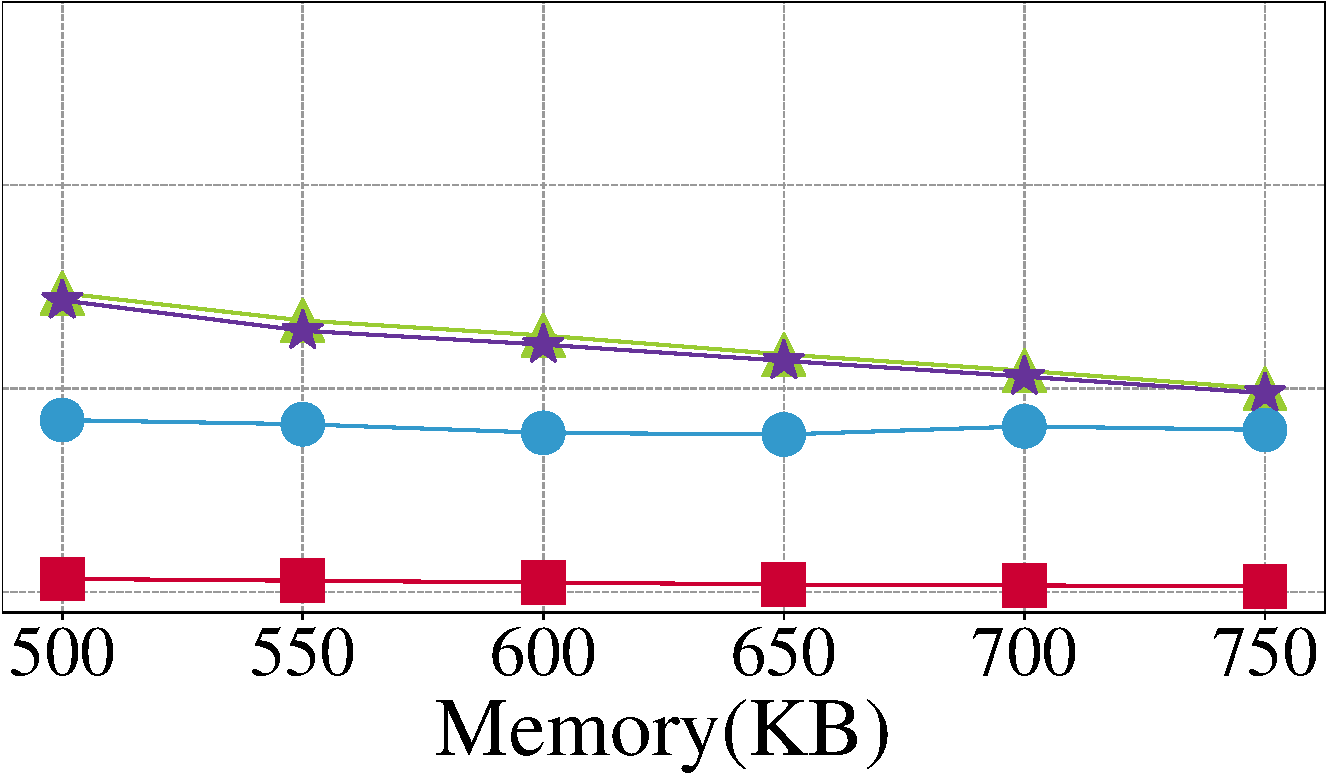
\includegraphics[width=0.95\textwidth, ]{Figures/sup/sup_are/_sup_ip6_are.pdf}
		\end{center}
		}
		\postfig 
		\adjustfigs
		\prefigcaption
		\label{sup_are_ip6}
		\postfigcaption
		\end{minipage}
	}
	%
	\subfigure[IP trace4]{
	    \begin{minipage}[t]{0.23\textwidth}{
		\prefig
		\begin{center}
		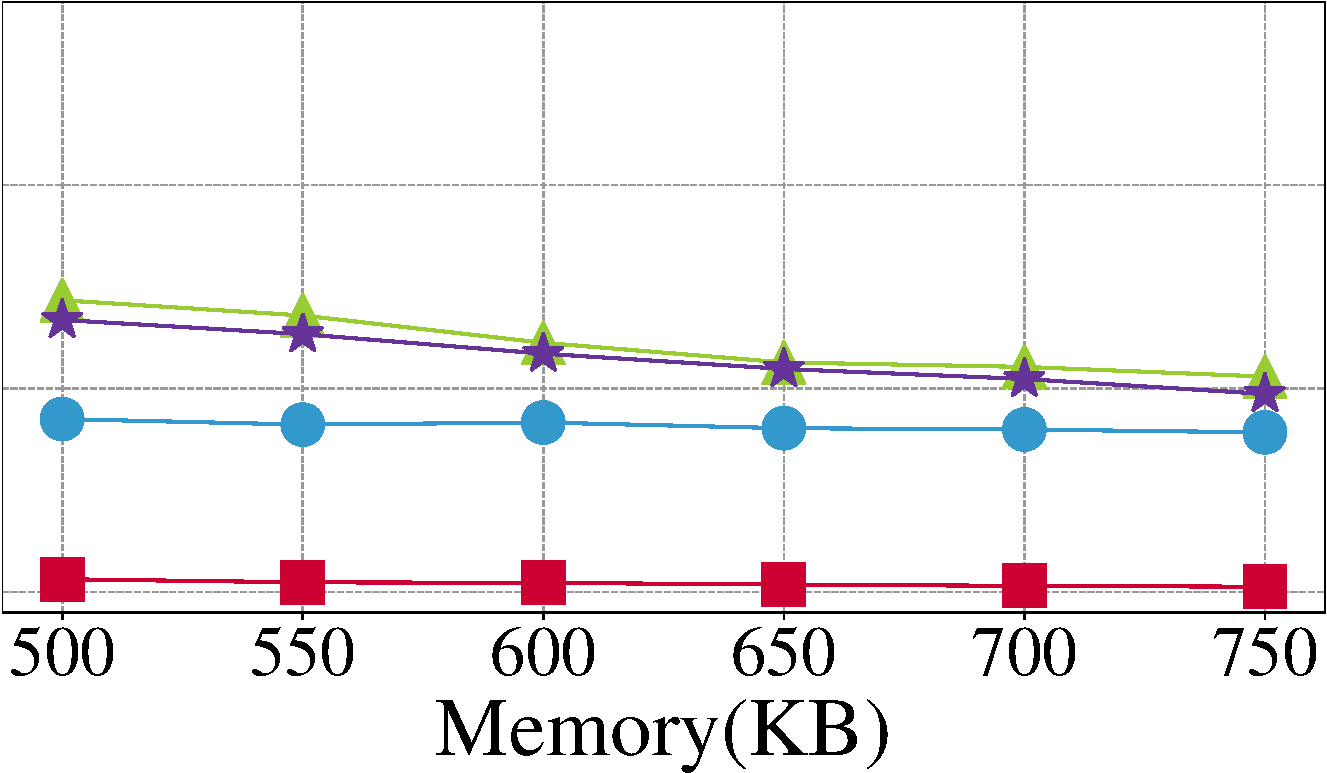
\includegraphics[width=0.95\textwidth, ]{Figures/sup/sup_are/_sup_ip8_are.pdf}
		\end{center}
		}
		\postfig 
		\adjustfigs
		\prefigcaption
		\label{sup_are_ip8}
		\postfigcaption
		\end{minipage}
	}
	%
	\vvv \vvv
    \caption{ARE of finding \tasktwo.}
	\label{sup_are}
\end{figure*}


\begin{figure*}[!ht]
	\centering
	%
	\subfigure[IP trace1]{
		\begin{minipage}[t]{0.255\textwidth}{
		\prefig
		\begin{center}
		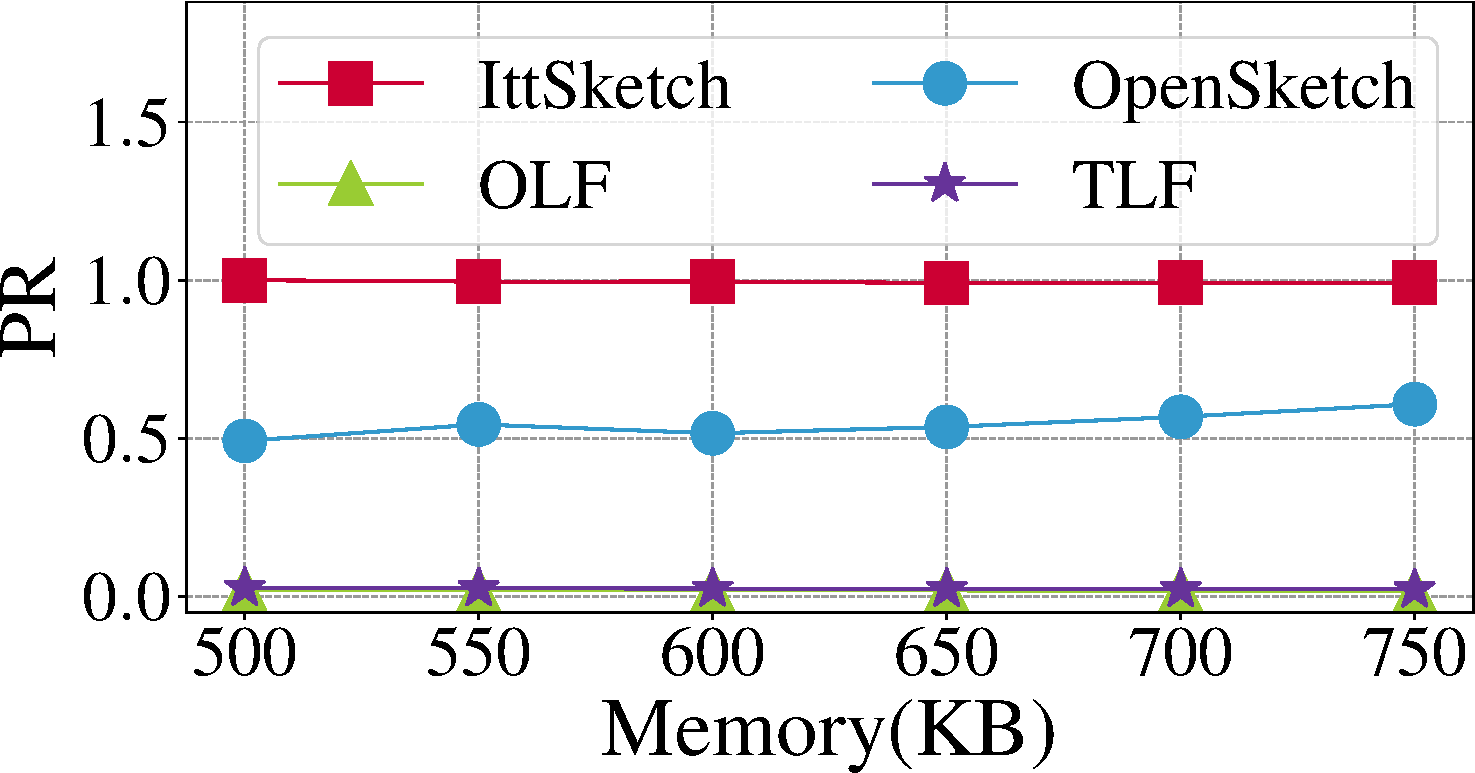
\includegraphics[width=0.95\textwidth, ]{Figures/sup/sup_pr/_sup_ip_pr.pdf}
		\end{center}
		}
		\postfig
		\adjustfigs
		\prefigcaption
		\label{sup_pr_ip}
		\postfigcaption
		\end{minipage}
	}
	%
	\subfigure[IP trace2]{
		\begin{minipage}[t]{0.23\textwidth}{
		\prefig
		\begin{center}		
		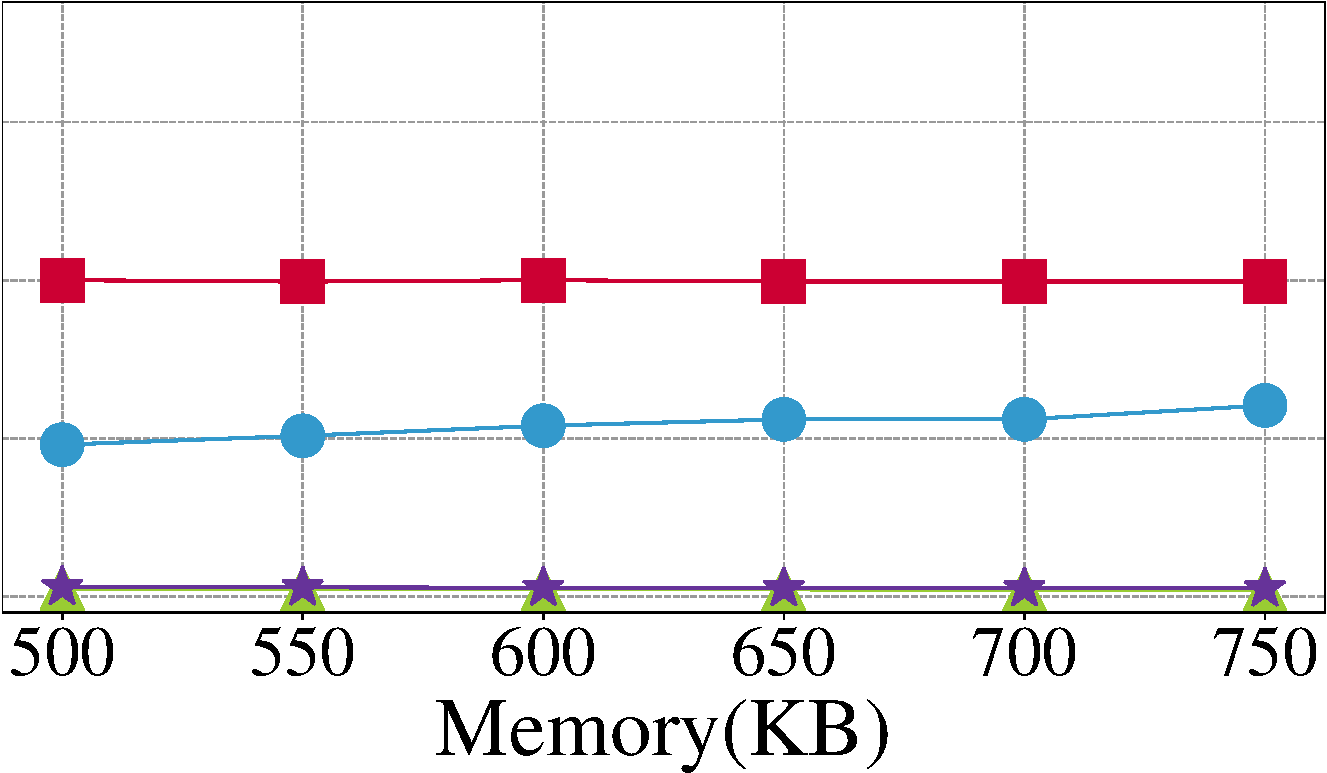
\includegraphics[width=0.95\textwidth, ]{Figures/sup/sup_pr/_sup_ip4_pr.pdf}
		\end{center}
		}
		\postfig 
		\adjustfigs
		\prefigcaption
		\label{sup_pr_ip4}
		\postfigcaption
		\end{minipage}
	}
	%
	\subfigure[IP trace3]{
		\begin{minipage}[t]{0.23\textwidth}{
		\prefig
		\begin{center}		
		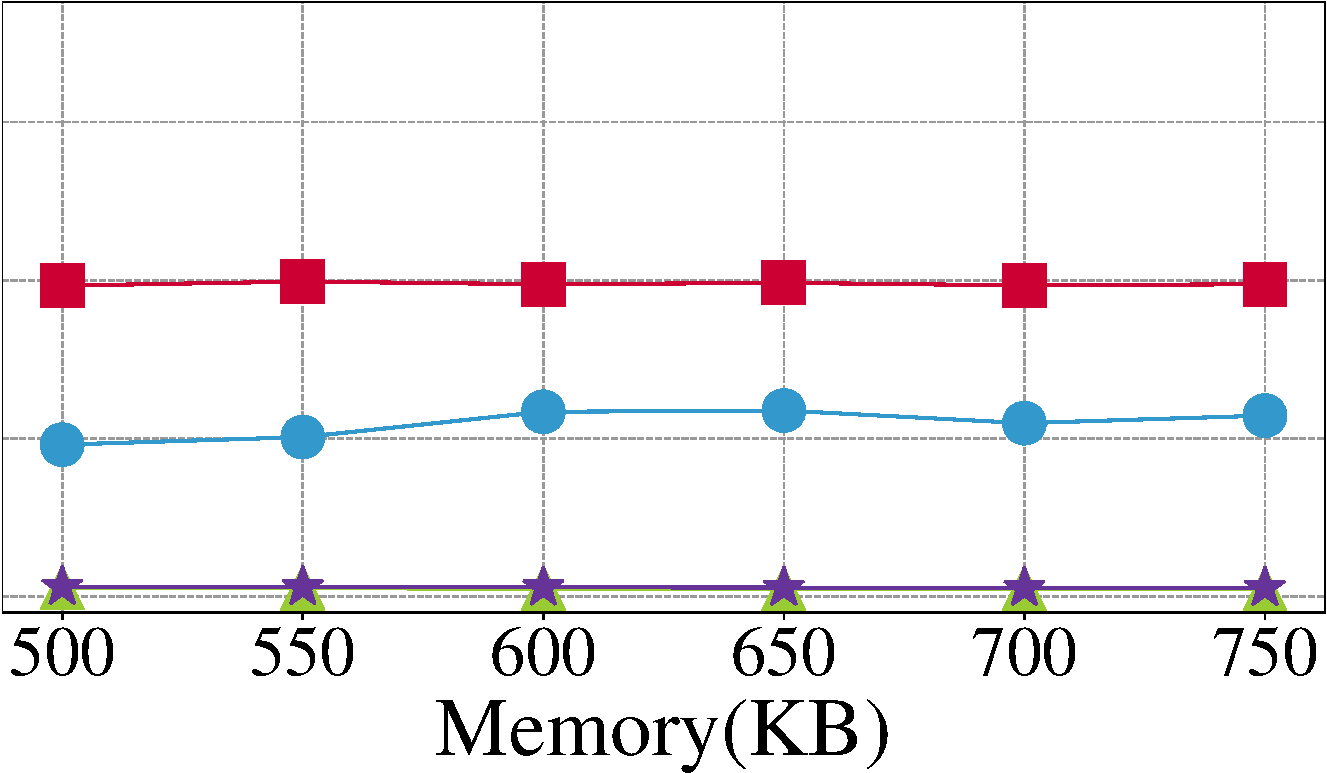
\includegraphics[width=0.95\textwidth, ]{Figures/sup/sup_pr/_sup_ip6_pr.pdf}
		\end{center}
		}
		\postfig 
		\adjustfigs
		\prefigcaption
		\label{sup_pr_ip6}
		\postfigcaption
		\end{minipage}
	}
	%
	\subfigure[IP trace4]{
		\begin{minipage}[t]{0.23\textwidth}{
		\prefig
		\begin{center}
		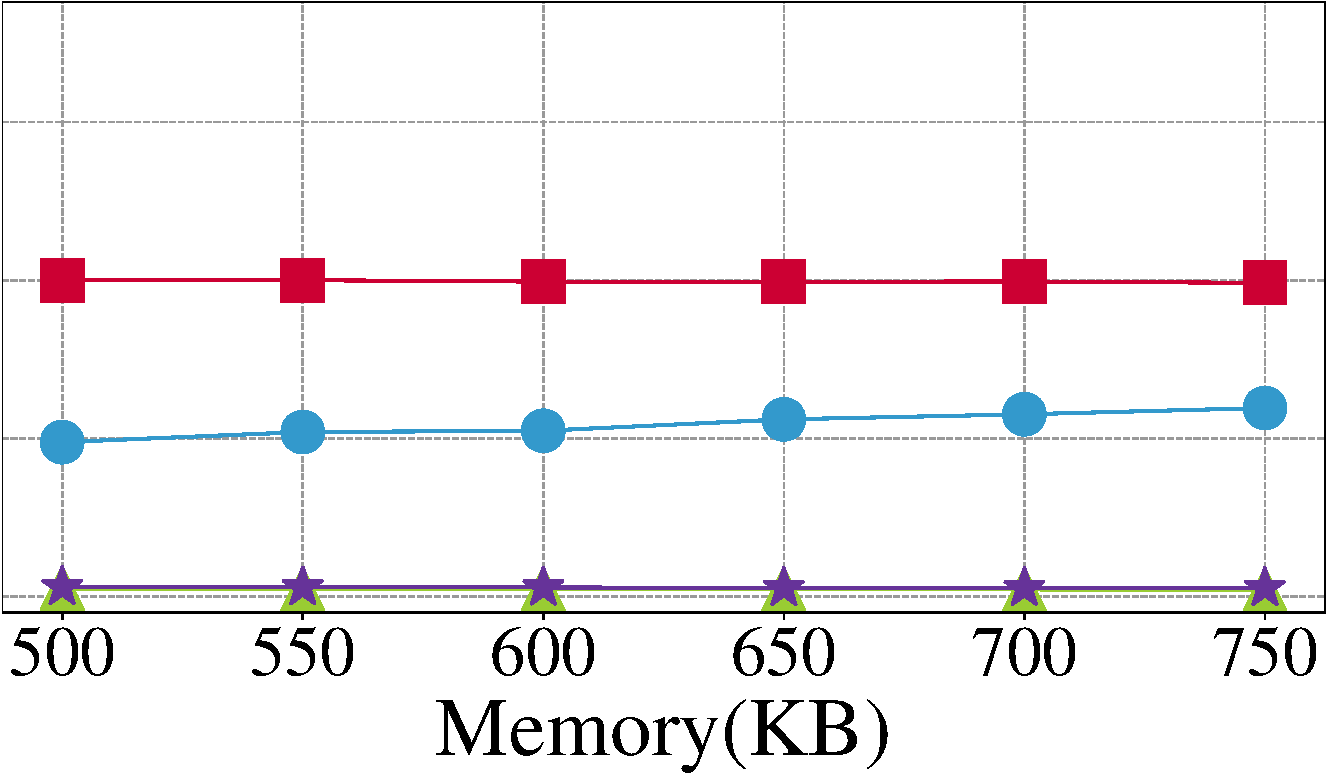
\includegraphics[width=0.95\textwidth, ]{Figures/sup/sup_pr/_sup_ip8_pr.pdf}
		\end{center}
		}
		\postfig 
		\adjustfigs
		\prefigcaption
		\label{sup_pr_ip8}
		\postfigcaption
		\end{minipage}
	}
	%
	\vvv \vvv
    \caption{PR of finding \tasktwo.}
	\label{sup_pr}
\end{figure*}

\begin{figure*}[!ht]
	\centering
	%
	\subfigure[IP trace1]{
		\begin{minipage}[t]{0.247\textwidth}{
		\prefig
		\begin{center}
		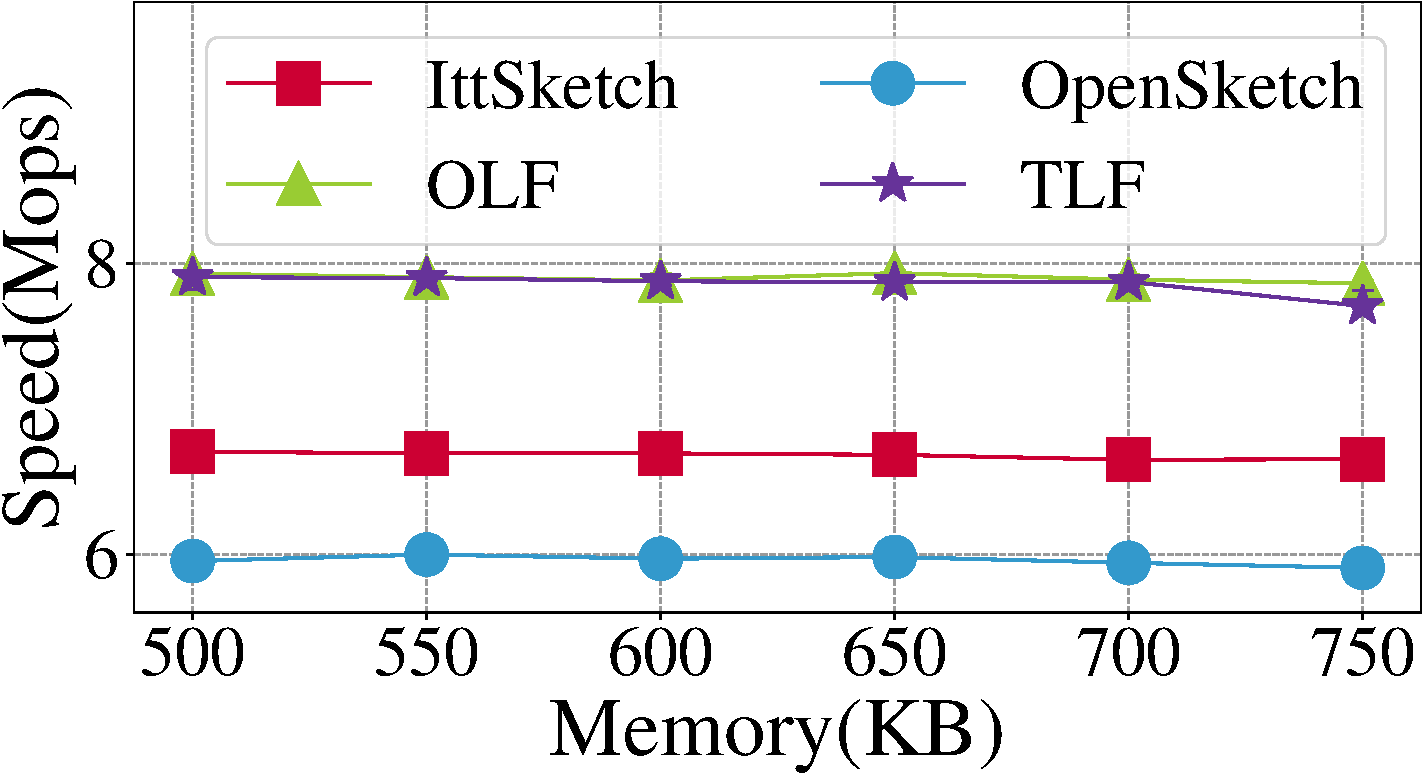
\includegraphics[width=0.95\textwidth, ]{Figures/sup/sup_speed/_sup_ip_speed.pdf}
	    \end{center}
	    }
		\postfig
		\adjustfigs
		\prefigcaption
		\label{sup_speed_ip}
		\postfigcaption
		\end{minipage}
	}
	%
	\subfigure[IP trace2]{
		\begin{minipage}[t]{0.23\textwidth}{				\prefig
		\begin{center}		
		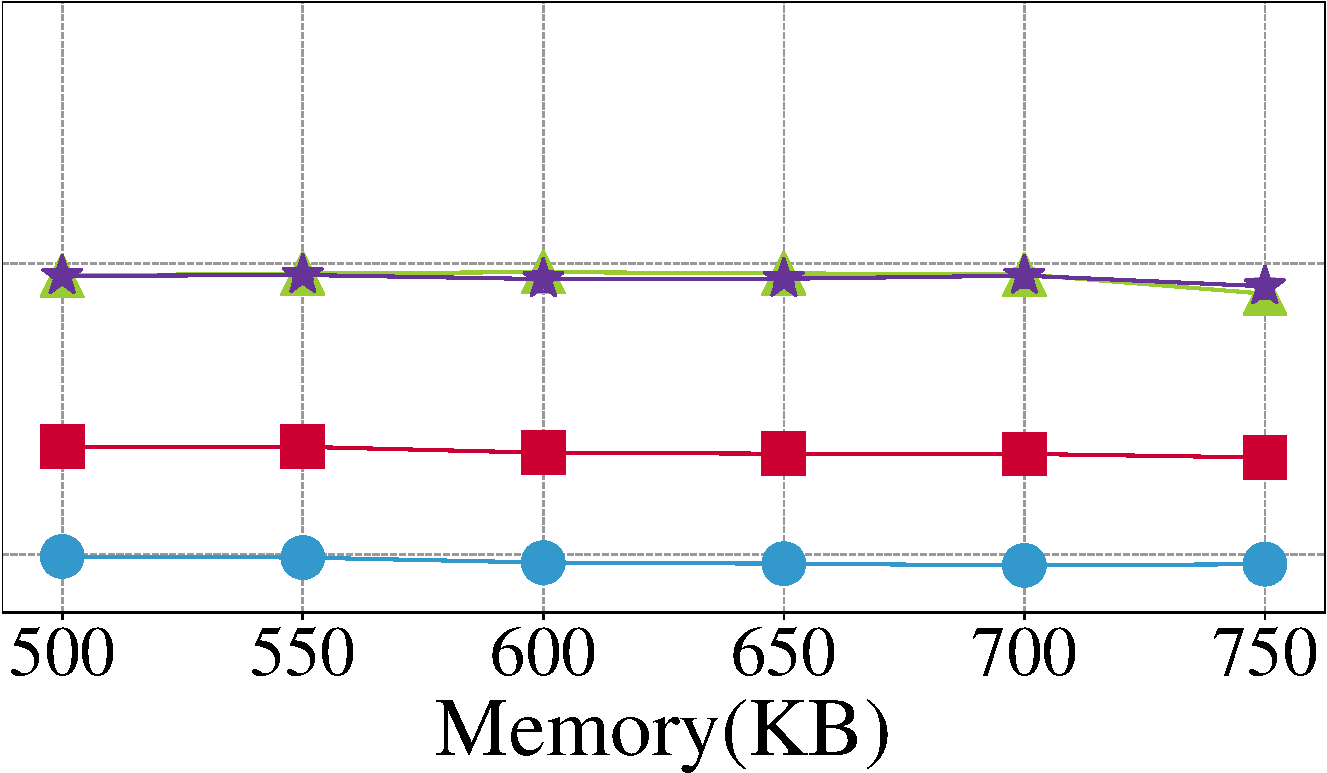
\includegraphics[width=0.95\textwidth, ]{Figures/sup/sup_speed/_sup_ip4_speed.pdf}
		\end{center}
		}
		\postfig 
		\adjustfigs
		\prefigcaption
		\label{sup_speed_ip4}
		\postfigcaption
		\end{minipage}
	}
	%
	\subfigure[IP trace3]{
		\begin{minipage}[t]{0.23\textwidth}{
		\prefig
		\begin{center}		
		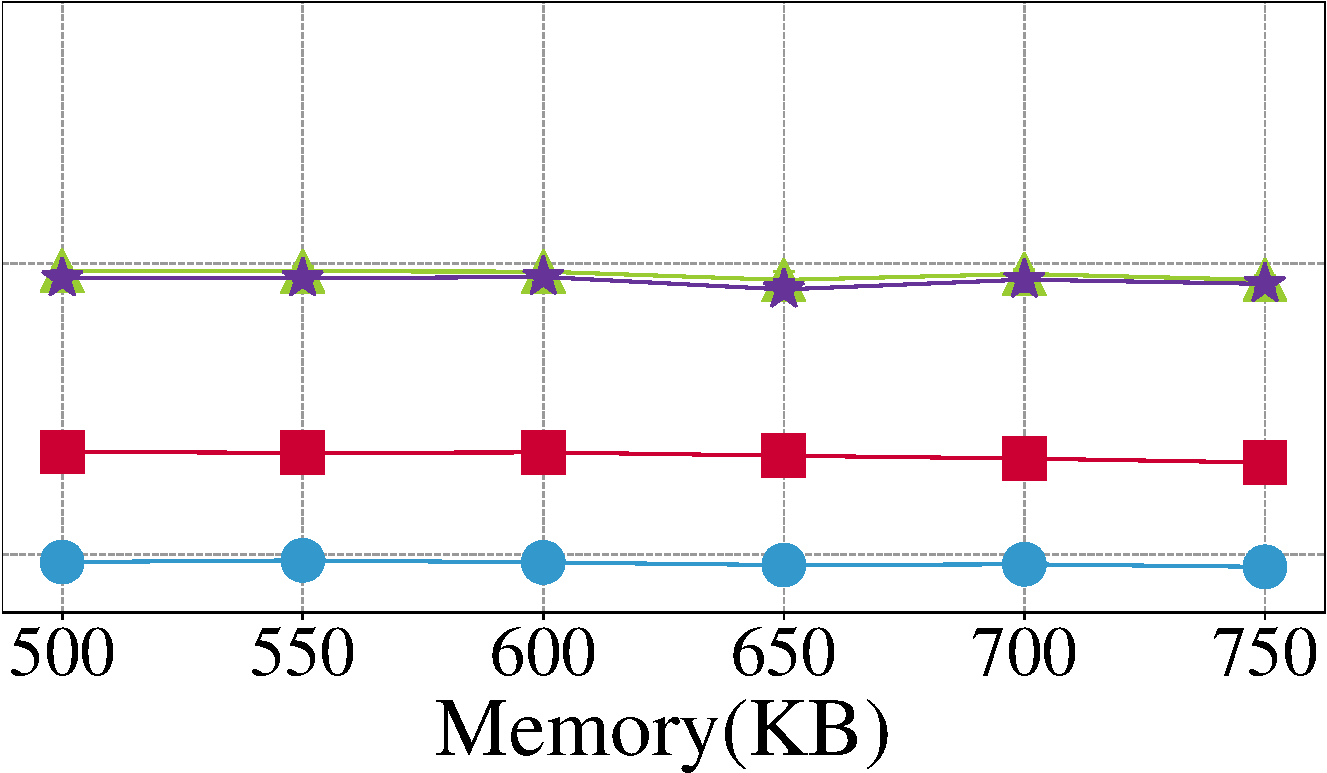
\includegraphics[width=0.95\textwidth, ]{Figures/sup/sup_speed/_sup_ip6_speed.pdf}
		\end{center}
		}
		\postfig 
		\adjustfigs
		\prefigcaption
		\label{sup_speed_ip6}
		\postfigcaption
		\end{minipage}
	}
	%
	\subfigure[IP trace4]{
		\begin{minipage}[t]{0.23\textwidth}{
		\prefig
		\begin{center}
		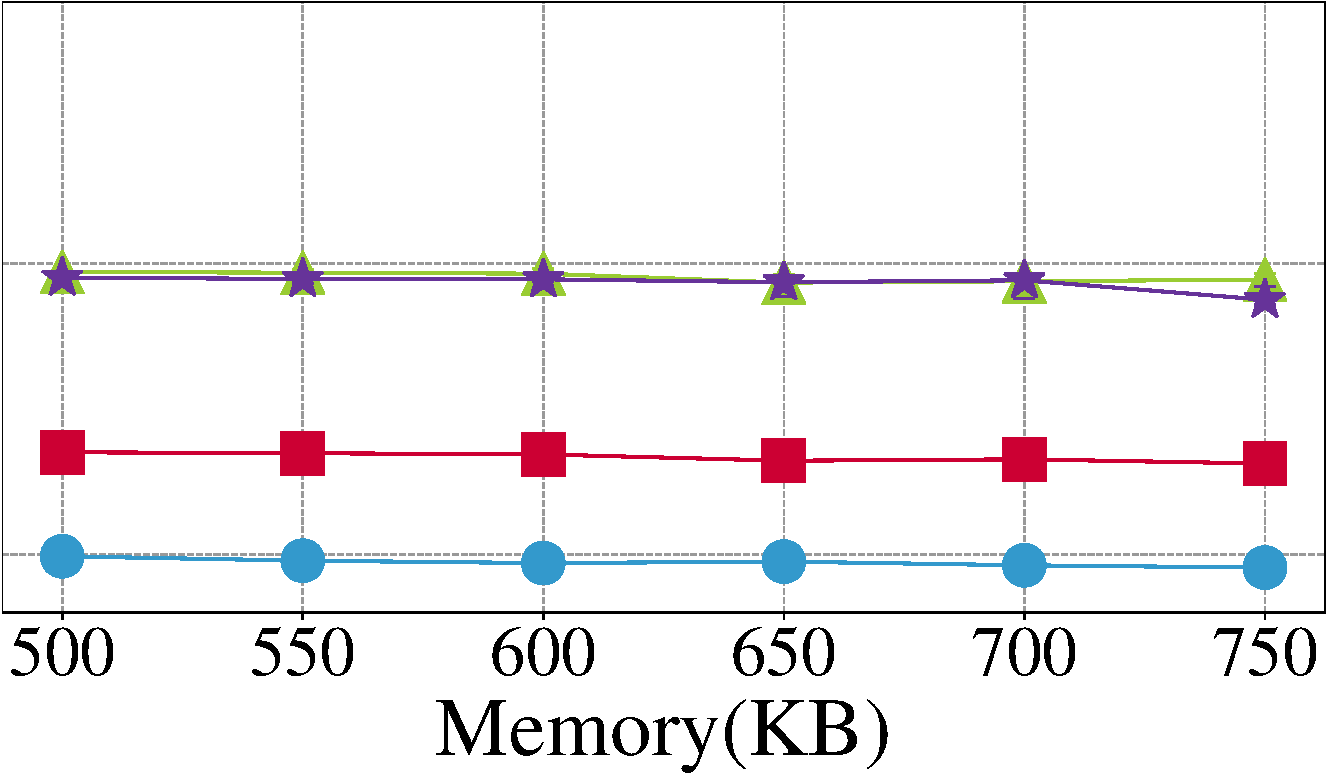
\includegraphics[width=0.95\textwidth, ]{Figures/sup/sup_speed/_sup_ip8_speed.pdf}
		\end{center}
		}
		\postfig 
		\adjustfigs
		\prefigcaption
		\label{sup_speed_ip8}
		\postfigcaption
		\end{minipage}
	}
	%
	\vvv \vvv
    \caption{Speed of finding \tasktwo.}
	\label{sup_speed}
\end{figure*}

%\presub
\subsection{Evaluation on Finding \taskfour} %\postsub
\label{eva_four}

\noindent\textbf{Parameter Setting:}
%We compare three frameworks: \sketchname, \EHname and \Splittername. For each frameworks, we using CM Sketch, CM-CU Sketch and Count Sketch approaches.
%
%We compare 5 approaches: CM \sketchname, CM-CU \sketchname, Count \sketchname, \EHname {} and \Splittername.
We compare 3 algorithms: \sketchname, \chafr\cite{flowradar}, and \chafrcf\cite{coldfilter}.
For \chafr{} and \chafrcf, the parameters are set according to the recommendation of the authors.
In the experiments, we compare PR, CR, and the insertion speed among the 3 algorithms. We vary the amount of memory from from 2MB to 4.5MB. We choose this range because \chafr{} cannot report any heavy changes if memory size is smaller. Also, we set the memory size of \sketchname{} to $1/20$ of the memory size of the other algorithms when we compare PR and CR. The reason for this is that when memory is larger than 2MB, the CR and PR of \sketchname{} are 1. 
%To compare these algorithms more conveniently, we reduce the memory size of \sketchname.


\noindent\textbf{PR (Figure~\ref{cha_pr_syn}-\ref{cha_pr_net}):}
We find that on three real-world datasets, the PR of \sketchname{} is around 4.1 times and 3.6 times higher than \chafr{} and \chafrcf. 
On the synthetic dataset, the PR of \chafr{} is 0 when its memory size is less than 2.5 MB. The PR of \sketchname{} is around 6.2 times higher than \chafrcf. 
			
			
\noindent\textbf{Speed (Figure~\ref{cha_speed_syn}-\ref{cha_speed_net}):}
We find that the insertion speed of \sketchname{} is around 2.1 times and 3 times faster than \chafr{} and \chafrcf{} on three real-world datasets and one synthetic dataset.

\noindent\textbf{CR (Figure~\ref{cha_cr_syn}-\ref{cha_cr_net}) in Appendix \ref{app:fig}:}
We find that, on three real-world datasets, the CR of \sketchname{} is around 64 times and 35 times higher than \chafr{} and \chafrcf. 
On the synthetic dataset, the CR of \chafr{} is 0 when its memory size is less than 2.5 MB. The CR of \sketchname{} is around 16 times higher than \chafrcf. 


\noindent\textbf{Summary:}
%
1) Although the memory size of \sketchname{} is only $1/20$ of other algorithms, the CR of \sketchname{} is often more than 0.98 when its memory size is more than 0.98 on three real-world datasets and one synthetic dataset. 
% Steve: broken sentence, please fix it.
In contrast, the CR of \chafr{} is often lower than 0.2 because it will decode few items if the memory size is too small.

2) The PR of \sketchname{} is lower than the PR of \sketchname~ in other datasets, for there are less differences between the two periods in the synthetic dataset. Therefore, we have to spend more space on finding heavy changes in the synthetic dataset. However, \sketchname{} still performs much better than \chafr{} and \chafrcf.
\begin{figure*}[!ht]
	\centering
	%
	\subfigure[Synthetic dataset]{
		\begin{minipage}[t]{0.2543\textwidth}{
		\prefig
		\begin{center}
		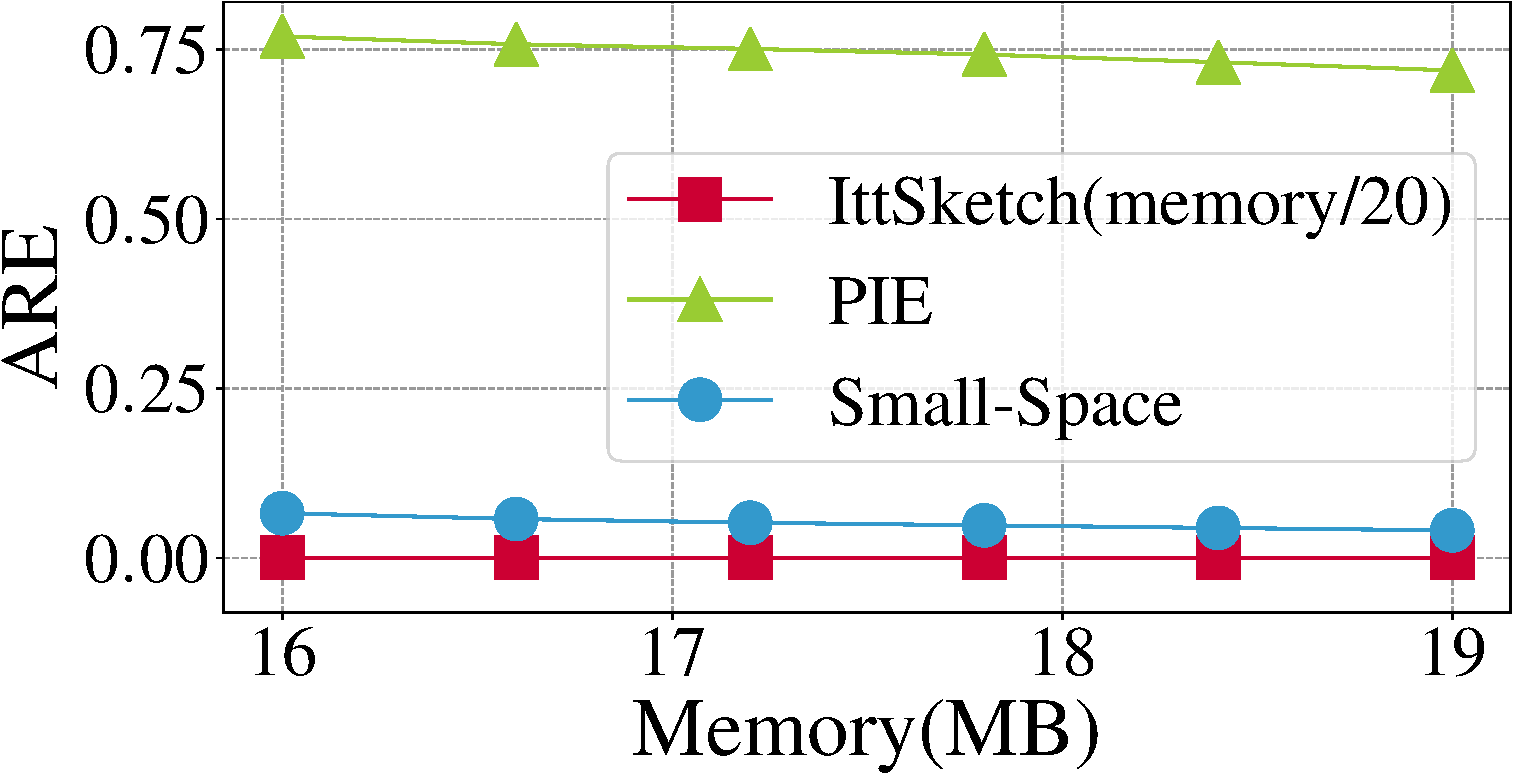
\includegraphics[width=0.95\textwidth, ]{Figures/per/per_are/per_syn_are-cropped.pdf}
		\end{center}
		}
		\postfig 
		\adjustfigs
		\prefigcaption
		\label{per_are_syn}
		\postfigcaption
		\end{minipage}
	}
	%
	\subfigure[IP trace]{
		\begin{minipage}[t]{0.225\textwidth}{
		\prefig
		\begin{center}
		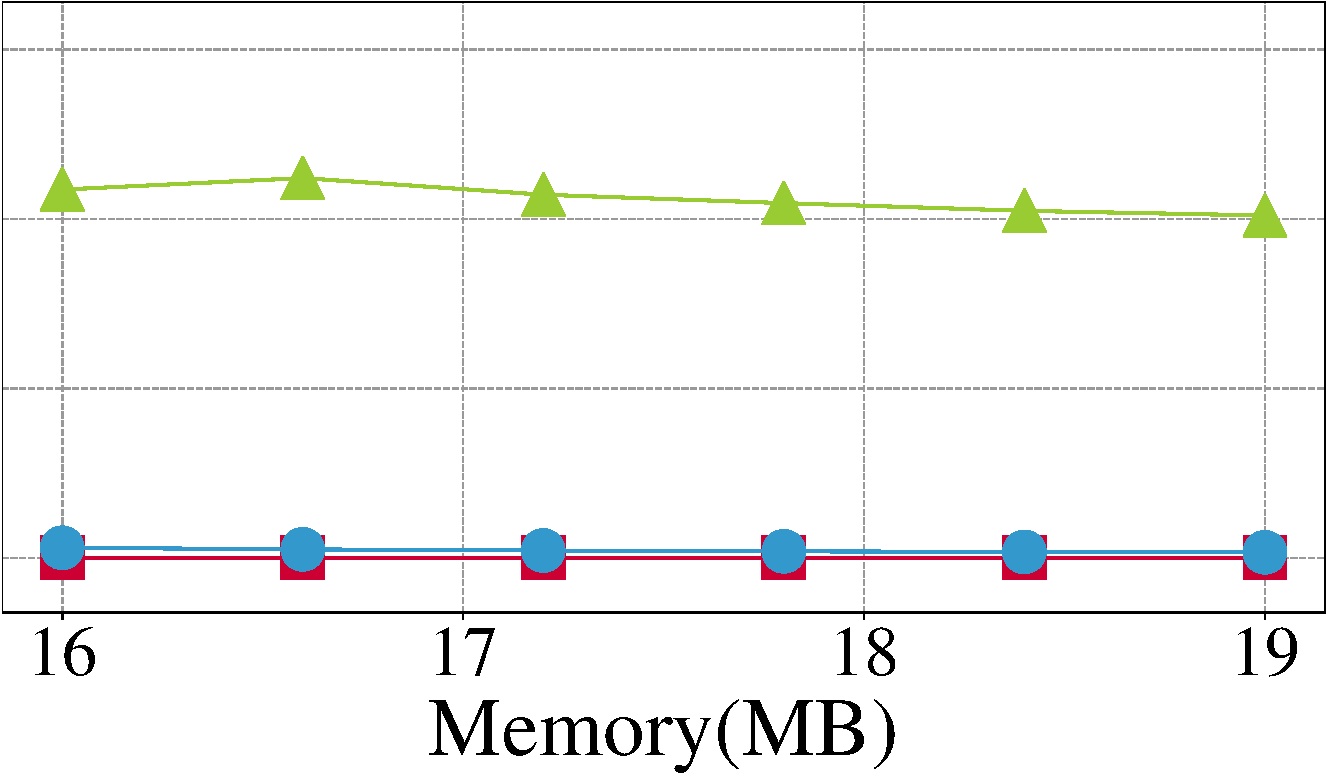
\includegraphics[width=0.95\textwidth, ]{Figures/per/per_are/per_ip_are-cropped.pdf}
		\end{center}
		}
		\postfig
		\adjustfigs
		\prefigcaption
		\label{per_are_ip}
		\postfigcaption
		\end{minipage}
	}
	%
	\subfigure[Web page]{
		\begin{minipage}[t]{0.225\textwidth}{
		\prefig
		\begin{center}		
		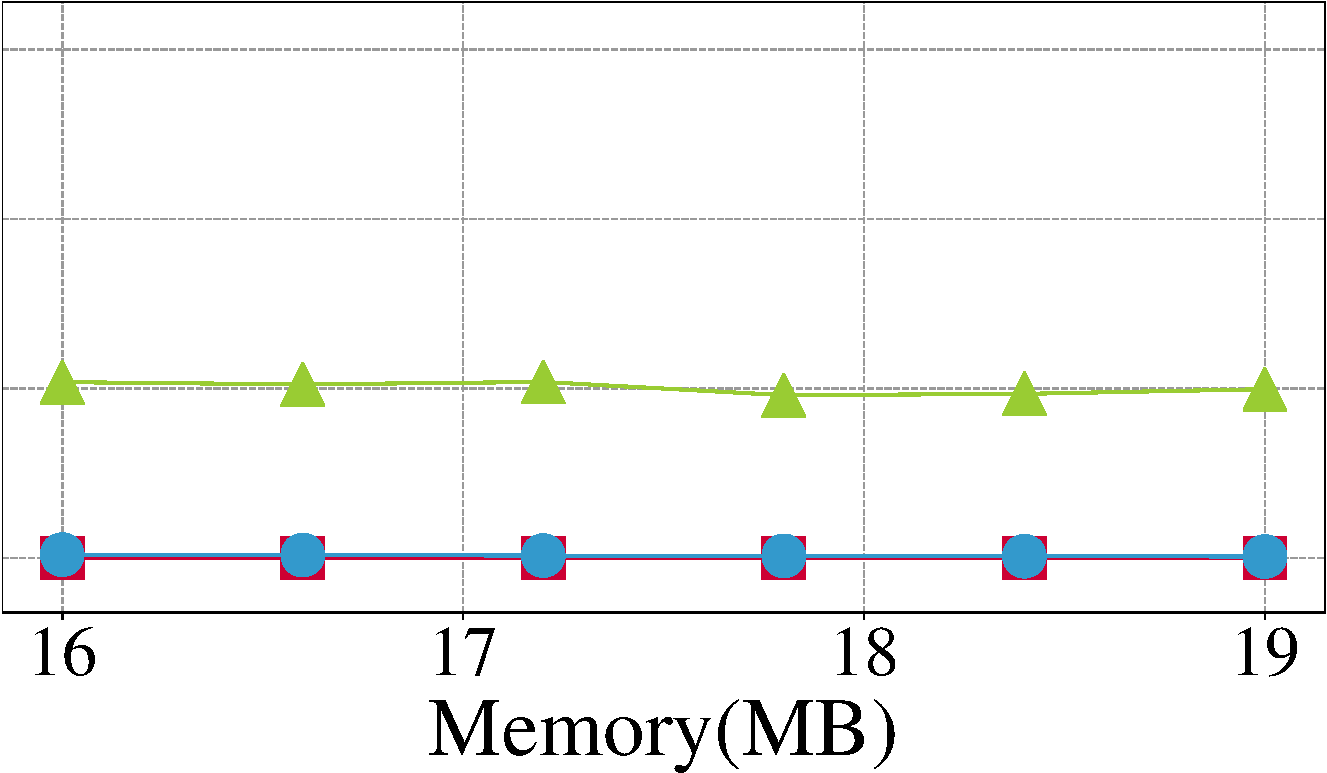
\includegraphics[width=0.95\textwidth, ]{Figures/per/per_are/per_web_are-cropped.pdf}\end{center}
		}
		\postfig 
		\adjustfigs
		\prefigcaption
		\label{per_are_web}
		\postfigcaption
		\end{minipage}
	}
	%
	\subfigure[Network dataset]{
		\begin{minipage}[t]{0.225\textwidth}{
		\prefig
		\begin{center}		
		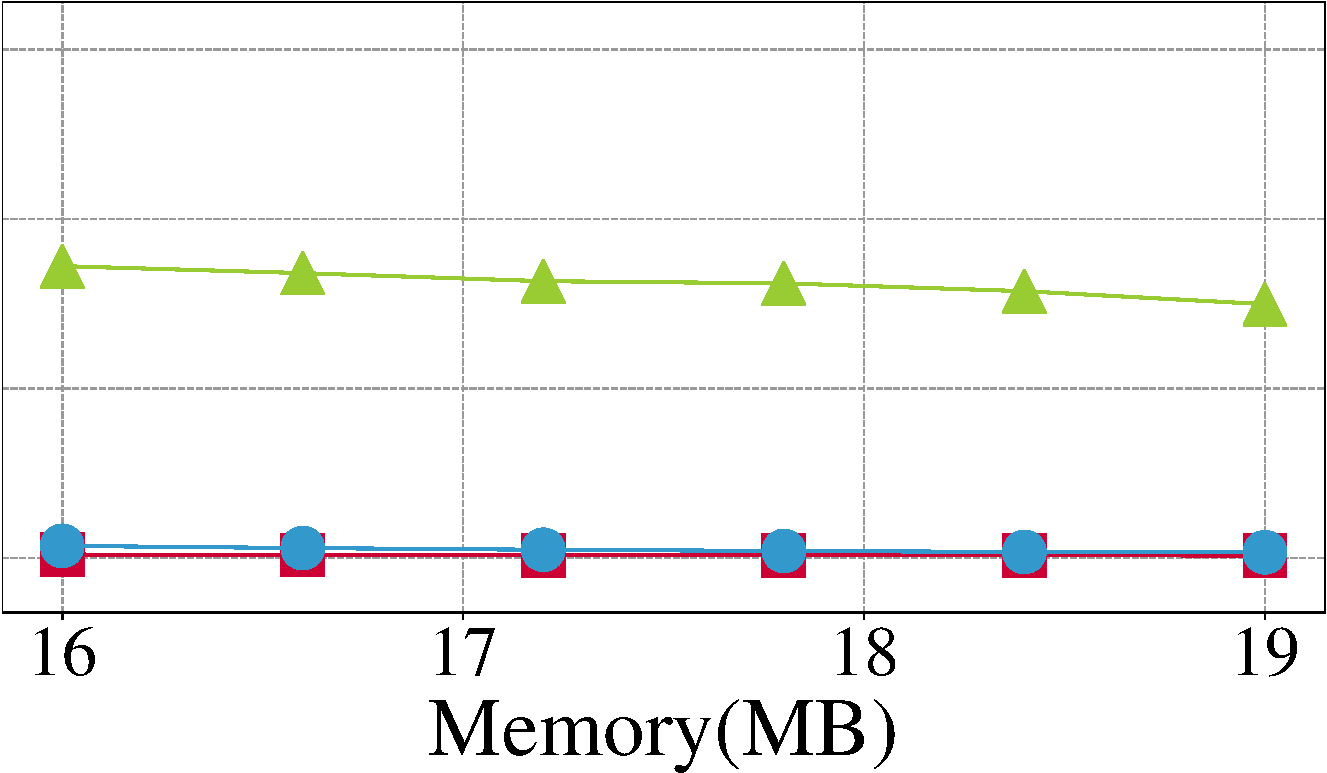
\includegraphics[width=0.95\textwidth, ]{Figures/per/per_are/per_net_are-cropped.pdf}
		\end{center}
		}
		\postfig 
		\adjustfigs
		\prefigcaption
		\label{per_are_net}
		\postfigcaption
		\end{minipage}
	}
	%
	\vvv \vvv
    \caption{ARE of finding \taskthree.}
	\label{per_are}
\end{figure*}

\begin{figure*}[!ht]
	\centering
	%
	\subfigure[Synthetic dataset]{
		\begin{minipage}[t]{0.255\textwidth}{
		\prefig
		\begin{center}
		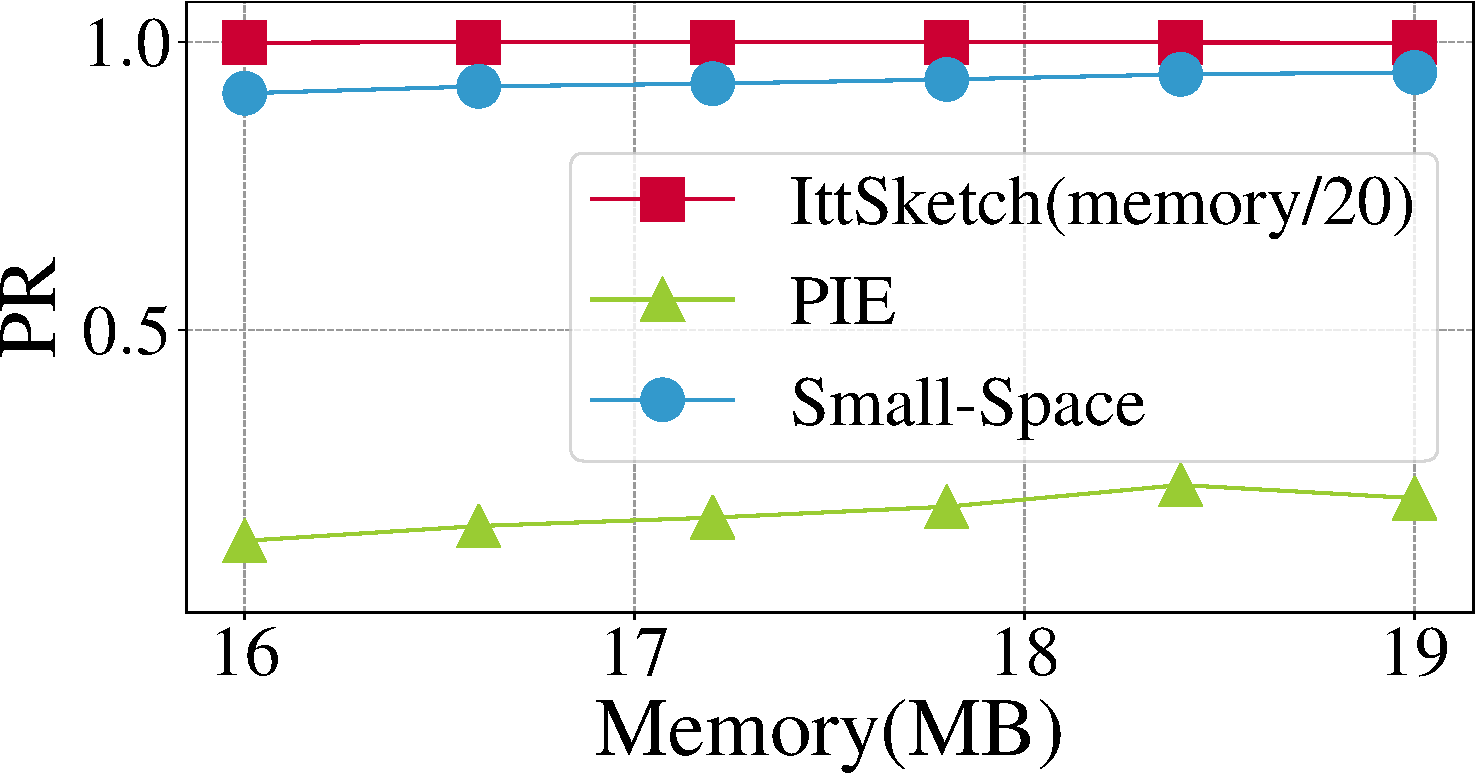
\includegraphics[width=0.95\textwidth, ]{Figures/per/per_pr/per_syn_pr-cropped.pdf}
		\end{center}
		}
		\postfig 
		\adjustfigs
		\prefigcaption
		\label{per_pr_syn}
		\postfigcaption
		\end{minipage}
	}
	%
	\subfigure[IP trace]{
		\begin{minipage}[t]{0.23\textwidth}{
		\prefig
		\begin{center}
		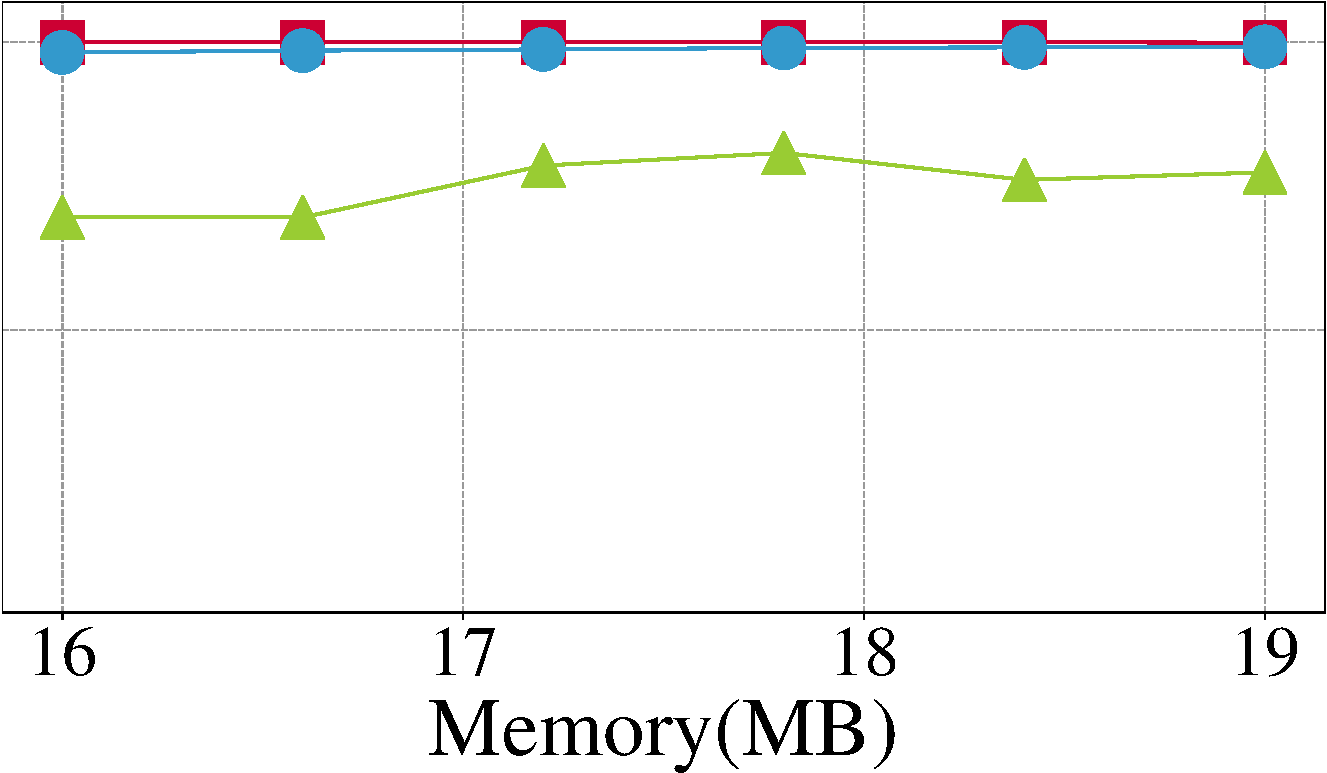
\includegraphics[width=0.95\textwidth, ]{Figures/per/per_pr/per_ip_pr-cropped.pdf}
		\end{center}
		}
		\postfig
		\adjustfigs
		\prefigcaption
		\label{per_pr_ip}
		\postfigcaption
		\end{minipage}
	}
	%
	\subfigure[Web page]{
		\begin{minipage}[t]{0.23\textwidth}{
		\prefig
		\begin{center}		
		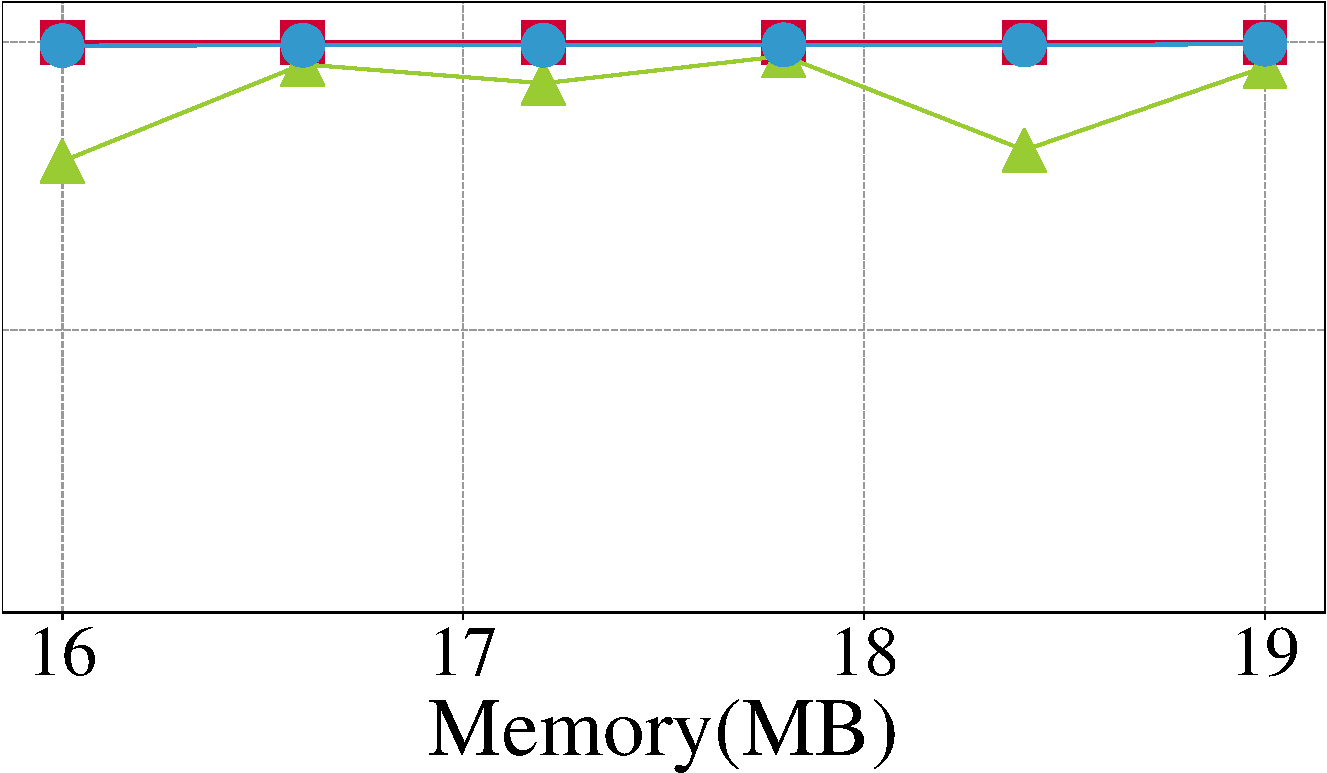
\includegraphics[width=0.95\textwidth, ]{Figures/per/per_pr/per_web_pr-cropped.pdf}
		\end{center}
		}
		\postfig 
		\adjustfigs
		\prefigcaption
		\label{per_pr_web}
		\postfigcaption
		\end{minipage}
	}
	%
	\subfigure[Network dataset]{
		\begin{minipage}[t]{0.23\textwidth}{
		\prefig
		\begin{center}		
		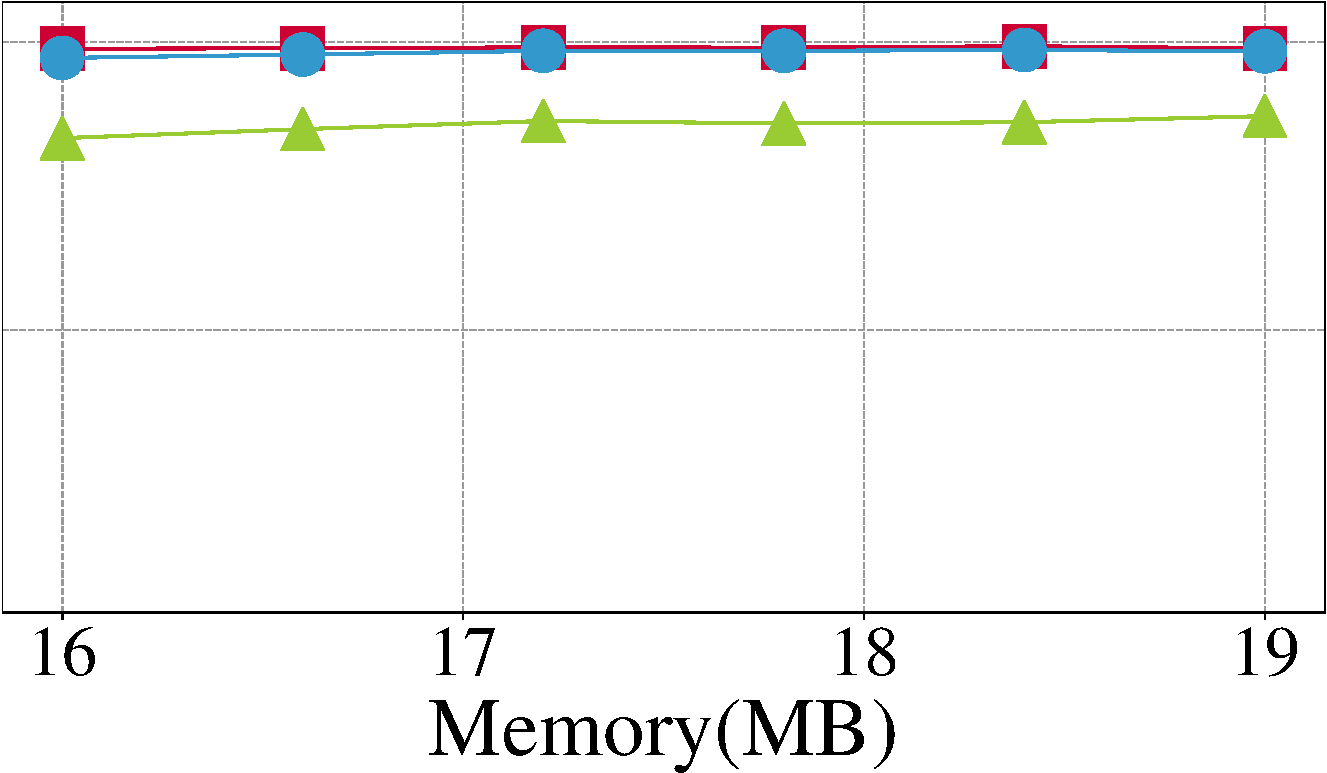
\includegraphics[width=0.95\textwidth, ]{Figures/per/per_pr/per_net_pr-cropped.pdf}
		\end{center}
		}
		\postfig 
		\adjustfigs
		\prefigcaption
		\label{per_pr_net}
		\postfigcaption
		\end{minipage}
	}
	%
	\vvv \vvv
    \caption{PR of finding \taskthree.}
	\label{per_pr}
\end{figure*}

\begin{figure*}[!ht]
	\centering
	%
	\subfigure[Synthetic dataset]{
		\begin{minipage}[t]{0.246126\textwidth}{
		\prefig
		\begin{center}
		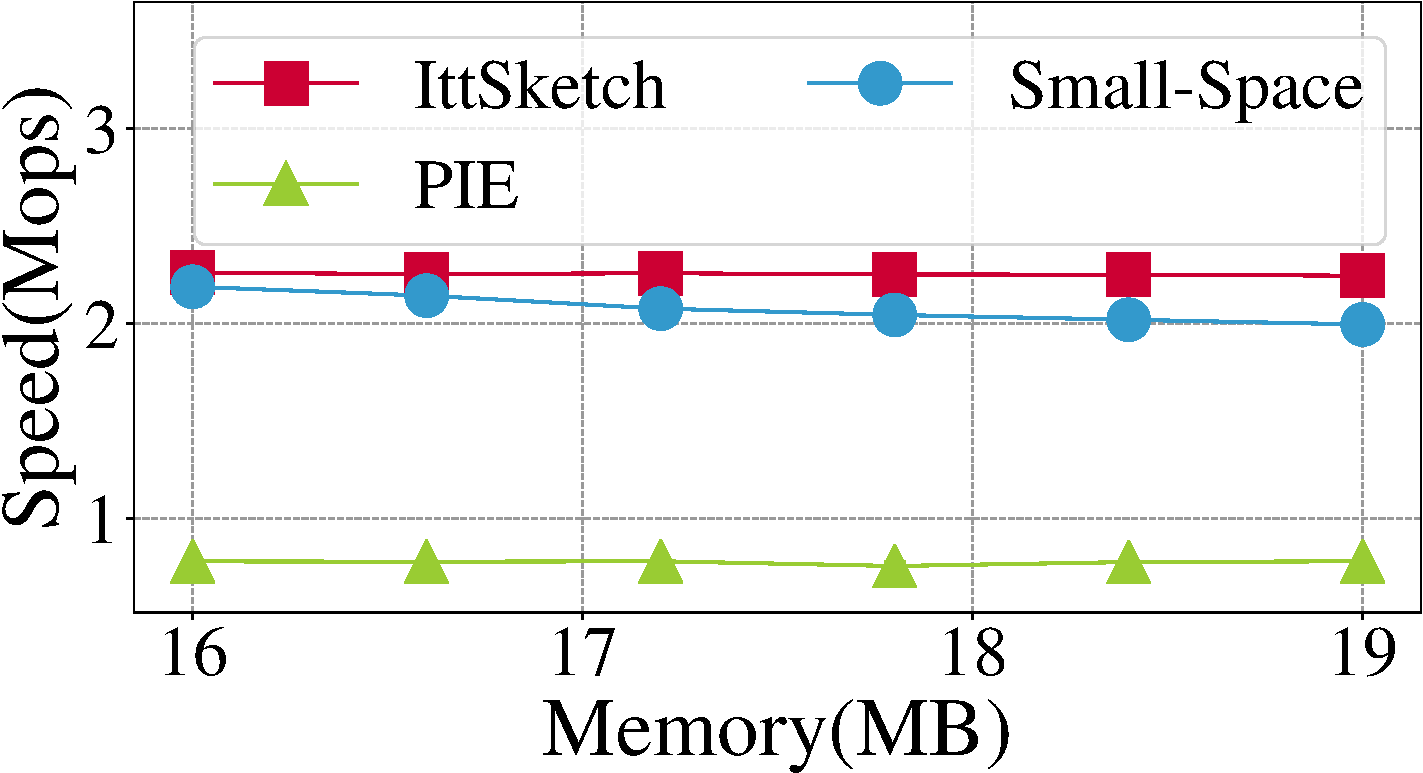
\includegraphics[width=0.95\textwidth, ]{Figures/per/per_speed/per_syn_speed-cropped.pdf}
		\end{center}
		}
		\postfig 
		\adjustfigs
		\prefigcaption
		\label{per_speed_syn}
		\postfigcaption
		\end{minipage}
	}
	%
	\subfigure[IP trace]{
		\begin{minipage}[t]{0.230622\textwidth}{
		\prefig
		\begin{center}
		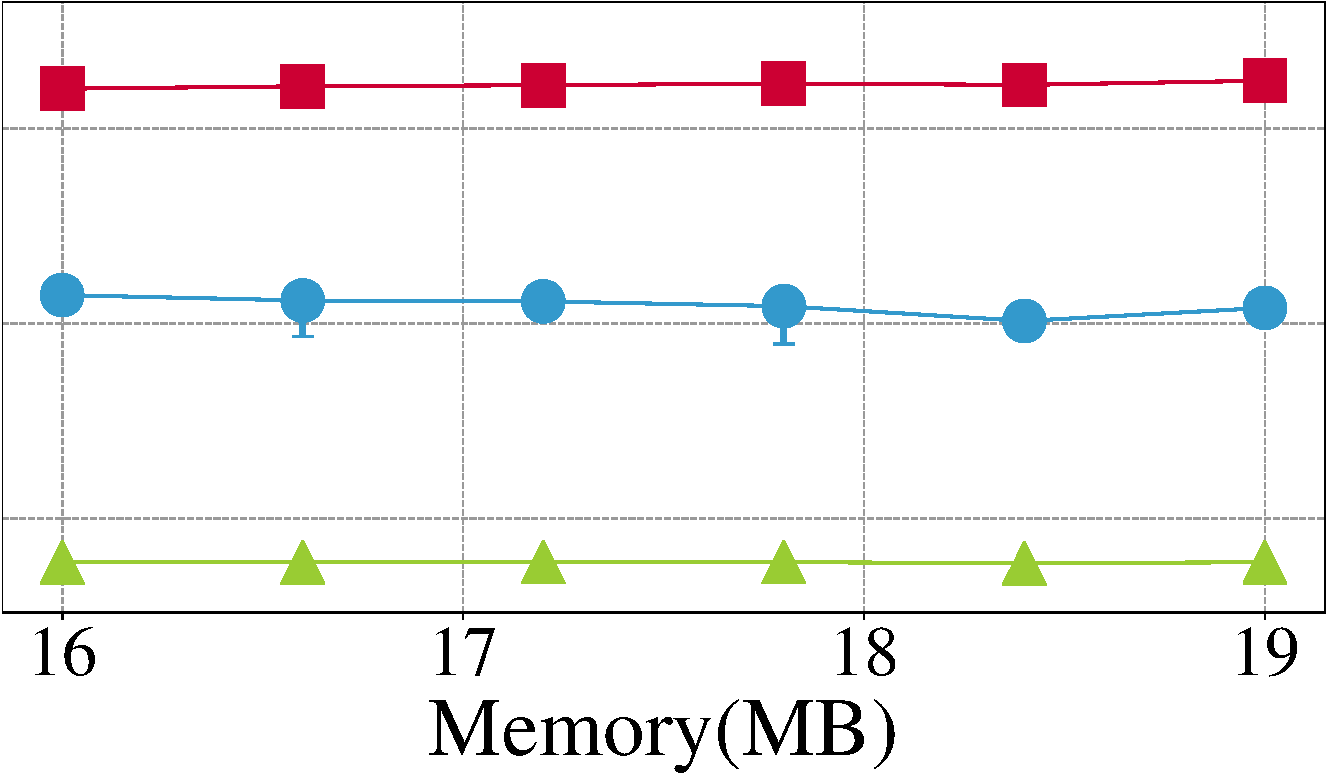
\includegraphics[width=0.95\textwidth, ]{Figures/per/per_speed/per_ip_speed-cropped.pdf}
		\end{center}
	    }
		\postfig
		\adjustfigs
		\prefigcaption
		\label{per_speed_ip}
		\postfigcaption
		\end{minipage}
	}
	%
	\subfigure[Web page]{
		\begin{minipage}[t]{0.230622\textwidth}{
		\prefig
		\begin{center}		
		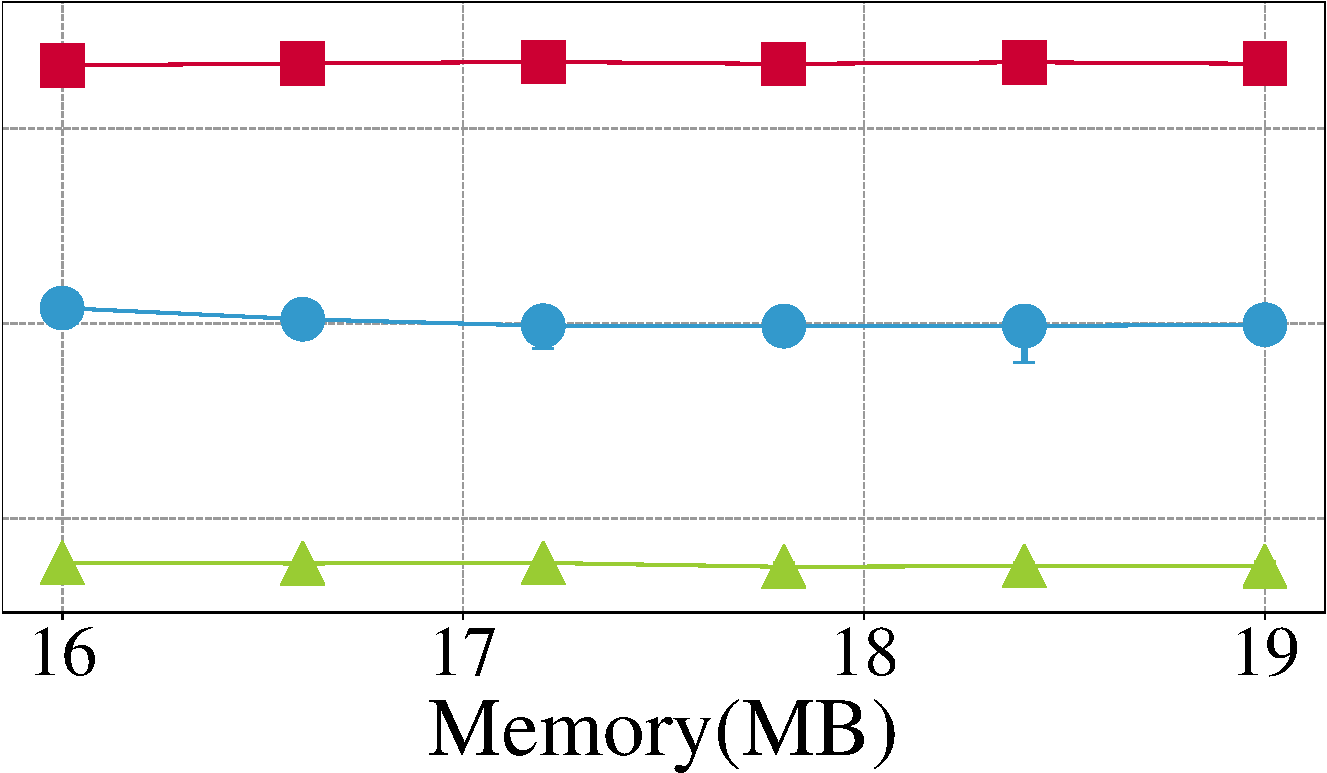
\includegraphics[width=0.95\textwidth, ]{Figures/per/per_speed/per_web_speed-cropped.pdf}
		\end{center}
		}
		\postfig 
		\adjustfigs
		\prefigcaption
		\label{per_speed_web}
		\postfigcaption
		\end{minipage}
	}
	%
	\subfigure[Network dataset]{
		\begin{minipage}[t]{0.230622\textwidth}{
		\prefig
		\begin{center}		
		\includegraphics[width=0.95\textwidth, ]{Figures/per/per_speed/per_net_speed-cropped.pdf}
		\end{center}
		}
		\postfig 
		\adjustfigs
		\prefigcaption
		\label{per_speed_net}
		\postfigcaption
		\end{minipage}
	}
	%
	\vvv \vvv
    \caption{Speed of finding \taskthree.}
	\label{per_speed}
\end{figure*}	

%\presub
\subsection{Evaluation on Finding \tasktwo} %\postsub
\label{eva_two}

\noindent\textbf{Parameter Setting:}
%We compare three frameworks: \sketchname, \EHname and \Splittername. For each frameworks, we using CM Sketch, CM-CU Sketch and Count Sketch approaches.
%
%We compare 5 approaches: CM \sketchname, CM-CU \sketchname, Count \sketchname, \EHname {} and \Splittername.
%
%
%原则:抄袭:不能连续六个一样的单词。。。
We compare 4 algorithms: \sketchname, \supolf\cite{superspreader}, \suptlf\cite{superspreader}, and \supopen\cite{opensketch}.
Let $z$ be the number of hash functions for the Bloom filter. For \sketchname{}, we set $z=4$.
For \supolf, \suptlf{}, and \supopen, the parameters are set according to the recommendation of the authors.
In the experiment, we compare AAE, ARE, PR, CR, and insertion speed among the 4 algorithms.
The memory size ranges from 500KB to 750KB. Because other algorithms often spend much memory on the hash table or bitmap, more memory is required for the experiment. Also, we split the IP Trace Dataset into 4 sub-datasets.
			
%% why different memory size for different interest...
%% cherry picker...

\noindent\textbf{ARE (Figure~\ref{sup_are_ip}-\ref{sup_are_ip8}):}
We find that the ARE of \sketchname{} is around 31 times, 30 times, and 18 times lower than \supolf, \suptlf{}, and \supopen{}, respectively.
			
\noindent\textbf{PR (Figure~\ref{sup_pr_ip}-\ref{sup_pr_ip8}):}
We find that \sketchname{} achieves a PR above 0.99 when the memory is more than 500KB. The PR of \sketchname{} is around 4.1 times, 3.4 times, and 1.9 times higher than \supolf, \suptlf{}, and \supopen{}, respectively.
			
			
\noindent\textbf{Speed (Figure~\ref{sup_speed_ip}-\ref{sup_speed_ip8}):}
We find that, on IP Trace datasets, the insertion speed of \sketchname{} is slower than \supolf{} and \suptlf{} but is faster than \supopen{}.

\noindent\textbf{AAE (Figure~\ref{sup_aae_ip}-\ref{sup_aae_ip8}) in Appendix \ref{app:fig}:}
We find that the AAE of \sketchname{} is around 14 times, 13.3 times, and 40 times lower than \supolf, \suptlf{}, and \supopen{}, respectively.

\noindent\textbf{CR (Figure~\ref{sup_cr_ip}-\ref{sup_cr_ip8}) in Appendix \ref{app:fig}:}
We find that the CR of \sketchname{} is around 1.4 times, 1.6 times, and 1.8 times higher than \supolf, \suptlf{}, and \supopen{}, respectively.

\noindent\textbf{Summary:} 
1) \sketchname{} is more accurate than other algorithms because other algorithms often spend much memory on the hash table or bitmap, which makes them unable to count items precisely.

2) Our results show that \sketchname{} achieves both high recall rate and high precision rate. Though \supolf{} and \suptlf{} report more correct instances than \supopen{}, they also report more wrong instances due to their low sample rate, making their precision rate lower than 0.03. 
\presub %\vvv
\subsection{Evaluation on Finding \taskthree} %\postsub
\label{eva_three}

\noindent\textbf{Parameter Setting:}
%We compare three frameworks: \sketchname, \EHname and \Splittername. For each frameworks, we using CM Sketch, CM-CU Sketch and Count Sketch approaches.
%
%We compare 5 approaches: CM \sketchname, CM-CU \sketchname, Count \sketchname, \EHname {} and \Splittername.
%
We compare 3 algorithms: \sketchname, \perpie\cite{persisitem}, and \perss\cite{smallspace}.
Let $z$ be the number of hash functions for the Bloom filter. For \sketchname{}, we set $z=3$.
For \perpie{} and \perss, the parameters are set according to the recommendation of the authors.
In the experiment, we compare AAE, ARE, PR, CR, and insertion speed among the 3 algorithms.
The memory size ranges from 16MB to 19MB. We choose this range because \perpie{} cannot report any interesting items on the synthetic dataset if memory size is less than 16MB. Also, we set the memory size of \sketchname{} to $1/20$ of the memory size of the other algorithms when we compare AAE, ARE, PR, and CR. 
We do this because when memory size is more than 16MB, the AAE and ARE of \sketchname{} are 0, and the CR and PR of \sketchname{} are 1. To compare these algorithms more conveniently, we reduce the memory size of \sketchname.
			
			
\noindent\textbf{ARE (Figure~\ref{per_are_syn}-\ref{per_are_net}):}
We find that, on three real-world datasets, the ARE of \sketchname{} is around 771 times and 50212 times lower than \perss{} and \perpie. On the synthetic dataset, the ARE of \sketchname{} is around 115 times and 1655 times lower than \perss{} and \perpie.  


\noindent\textbf{PR (Figure~\ref{per_pr_syn}-\ref{per_pr_net}):}
We find that, on three real-world datasets, the PR of \sketchname{} is around 1.01 times and 1.23 times higher than \perss{} and \perpie. On the synthetic dataset, the PR of \sketchname{} is around 1.08 times and 6 times higher than \perss{} and \perpie.  
			
			
\noindent\textbf{Speed (Figure~\ref{per_speed_syn}-\ref{per_speed_net}):}
We find that the insertion speed of \sketchname{} is around 1.4 times and 4 times faster than \perss{} and \perpie{} on three real-world datasets and one synthetic dataset.

\noindent\textbf{AAE (Figure~\ref{per_aae_syn}-\ref{per_aae_net}) in Appendix \ref{app:fig}:}
We find that, on three real-world datasets, the AAE of \sketchname{} is around 698 times and 53543 times lower than \perss{} and \perpie. On the synthetic dataset, the AAE of \sketchname{} is around 167 times and 6095 times lower than \perss{} and \perpie. 

\noindent\textbf{CR (Figure~\ref{per_cr_syn}-\ref{per_cr_net}) in Appendix \ref{app:fig}:}
We find that, on three real-world datasets, the CR of \sketchname{} is around 1.03 times and 33 times higher than \perss{} and \perpie. On the synthetic dataset, the CR of \sketchname{} is around 1.05 times and 33 times higher than \perss{} and \perpie.  

\noindent\textbf{Summary:}
%
1) Although the memory size of \sketchname{} is only $1/20$ of the other algorithms, it still performs much better. The ARE of \sketchname{} is lower than 0.005 when its memory size is more than 800KB on three real-world datasets and one synthetic dataset.

2) The PR and CR of \sketchname{} are often more than 0.99 when its memory size is more than 800KB on three real-world datasets and one synthetic dataset. The PR and CR of \perss{} are often more than 0.95 when its memory size is more than 16MB on three real-world datasets and one synthetic dataset. However, the CR of \perpie{} is often lower than 0.2 because it wastes much of the space to record the items in every period.

3) \sketchname{} can achieve higher insertion speed compared to \perss{} and \perpie. Also, \sketchname{} will not be slower when its memory use increases. In contrast, \perss{} slows down as memory use increases.
{\color{reviewA}
\presub
\subsection{Evaluation on Distributions and Arrival Orders} \postsub
\label{eva_data}

\begin{figure}[!ht]
	\centering
	\subfigure[Impact of dataset distribution]{
		\begin{minipage}[t]{0.22\textwidth}{
			\prefig
			\begin{center}
			\includegraphics[width=\textwidth, ]{Figures/dataset/skew_out_are-cropped.pdf}
			\end{center}}
			\postfig 
			\adjustfigs
			\prefigcaption
			\label{skew_are}
			\postfigcaption
		\end{minipage}
	}
	\subfigure[Impact of arrival order]{
		\begin{minipage}[t]{0.22\textwidth}{
		    \prefig
			\begin{center}
			\includegraphics[width=\textwidth, ]{Figures/dataset/order_out_are-cropped.pdf}
			\end{center}}
			\postfig
			\adjustfigs
			\prefigcaption
			\label{order_are}
			\postfigcaption
		\end{minipage}}
	\vvv \vvv
    \caption{Accuracy vs. skewness and item arrival order. Given a dataset, ``SHF'' refers to that the Second Half of items go First.}
	\label{dataset}
\end{figure}

In this subsection, we show how the dataset distribution and the arrival order of items affect the accuracy of PRI.

\noindent\textbf{Parameter Setting:}
We use synthetic datasets whose skewness varies from 0.3 to 3.0 to show the impact of dataset distribution to InterestSketch. We use the dataset whose skewness is 1.5 and three different orders to show the impact of the arrival order of items. Three different orders are the original order, the reversed order, and the Second Half First (SHF).
%
In this experiment, we plot the change of ARE of InterestSketch to show the impact.
The size of memory used ranges from 40KB to 140KB. We choose this range because using small memory can clearly expose the impact.

\noindent\textbf{Impact of dataset distribution (Figure~\ref{skew_are}):}
Our results show that the ARE of \sketchname{} is often lower than 0.01, and changes a little bit, especially when skewness is larger than 0.6.

\noindent\textbf{Impact of arrival orders (Figure~\ref{order_are}):}
Our results show that arrival orders indeed make some effects on the ARE of our \sketchname, but the effect is also not significant.
Because PRI replaces the minimum counter with a probability, the fluctuation of ARE in a certain range is reasonable.
}

{\color{reviewD}
\presub
\subsection{Extending SS and USS for Other Tasks} %\postsub
\label{eva_other}

\noindent\textbf{Parameter Setting:}
In this subsection, we use Unbiased SS\cite{unbiasedsketch} and SS\cite{spacesaving} to address the other three kinds of tasks.
We use \textit{IP Trace Dataset} to evaluate because only IP Trace Dataset can be used for finding Super-Spreaders.
			
\begin{figure*}[!ht]
	\centering
	\subfigure[CR of Finding \taskfour]{
		\begin{minipage}[t]{0.23\textwidth}{
			\prefig
			\begin{center}
			\includegraphics[width=\textwidth, ]{Figures/other/other_cha_cr-cropped.pdf}
			\end{center}}
			\postfig 
			\adjustfigs
			\prefigcaption
			\label{other_cha_cr}
			\postfigcaption
		\end{minipage}
	}
	\subfigure[PR of Finding \taskfour]{
		\begin{minipage}[t]{0.23\textwidth}{
		    \prefig
			\begin{center}
			\includegraphics[width=\textwidth, ]{Figures/other/other_cha_pr-cropped.pdf}
			\end{center}}
			\postfig
			\adjustfigs
			\prefigcaption
			\label{other_cha_pr}
			\postfigcaption
		\end{minipage}}
	\subfigure[ARE of Finding \tasktwo]{
		\begin{minipage}[t]{0.23\textwidth}{
			\prefig
			\begin{center}
			\includegraphics[width=\textwidth, ]{Figures/other/other_sup_are-cropped.pdf}
			\end{center}}
			\postfig 
			\adjustfigs
			\prefigcaption
			\label{other_sup_are}
			\postfigcaption
		\end{minipage}
	}
	\subfigure[ARE of Finding \taskthree]{
		\begin{minipage}[t]{0.23\textwidth}{
		    \prefig
			\begin{center}
			\includegraphics[width=\textwidth, ]{Figures/other/other_per_are-cropped.pdf}
			\end{center}}
			\postfig
			\adjustfigs
			\prefigcaption
			\label{other_per_are}
			\postfigcaption
		\end{minipage}}
	\vvv \vvv
    \caption{Accuracy comparison of InterestSketch, SS, and USS for other three tasks.}
	\label{other}
\end{figure*}

\begin{figure*}[!ht]
	\centering
	\subfigure[Latency of Finding \taskone]{
		\begin{minipage}[t]{0.23\textwidth}{
			\prefig
			\begin{center}
			\includegraphics[width=\textwidth, ]{Figures/latency/fre_ip_latency-cropped.pdf}
			\end{center}}
			\postfig 
			\adjustfigs
			\prefigcaption
			\label{fre_ip_latency}
			\postfigcaption
		\end{minipage}
	}
	\subfigure[Latency of Finding \taskfour]{
		\begin{minipage}[t]{0.23\textwidth}{
		    \prefig
			\begin{center}
			\includegraphics[width=\textwidth, ]{Figures/latency/cha_ip_latency-cropped.pdf}
			\end{center}}
			\postfig
			\adjustfigs
			\prefigcaption
			\label{cha_ip_latency}
			\postfigcaption
		\end{minipage}
	}
	\subfigure[Latency of Finding \tasktwo]{
		\begin{minipage}[t]{0.23\textwidth}{
			\prefig
			\begin{center}
			\includegraphics[width=\textwidth, ]{Figures/latency/sup_ip_latency-cropped.pdf}
			\end{center}}
			\postfig 
			\adjustfigs
			\prefigcaption
			\label{sup_ip_latency}
			\postfigcaption
		\end{minipage}
	}
	\subfigure[Latency of Finding \taskthree]{
		\begin{minipage}[t]{0.23\textwidth}{
		    \prefig
			\begin{center}
			\includegraphics[width=\textwidth, ]{Figures/latency/per_ip_latency-cropped.pdf}
			\end{center}}
			\postfig
			\adjustfigs
			\prefigcaption
			\label{per_ip_latency}
			\postfigcaption
		\end{minipage}
	}
	%\vvv \vvv
    \caption{Latency of four tasks.}
	\label{latency}
\end{figure*}
			
\noindent\textbf{CR and PR of Finding \taskfour{} (Figure~\ref{other_cha_cr}-\ref{other_cha_pr}):}
We can find that, the CR of \sketchname{} is around 2.67 times and 2.45 times higher than SS and Unbiased SS. According to Figure \ref{other_cha_pr}, the PR of \sketchname{} is around 9.33 times and 8.17 times higher than SS and Unbiased SS.

\noindent\textbf{ARE of Finding \tasktwo{} (Figure~\ref{other_sup_are}):}
We find that, the ARE of \sketchname{} is around 115.5 times and 126.7 times higher than SS and Unbiased SS. The ARE of \sketchname{} is often lower than 0.04, while the ARE of SS and Unbiased SS is often higher than 2.6.

\noindent\textbf{ARE of Finding \taskthree{} (Figure~\ref{other_per_are}):}
Our results show that the ARE of \sketchname{} is around 2347 times and 2000 times higher than SS and Unbiased SS. The ARE of \sketchname{} is often lower than 0.006, while the ARE of SS and Unbiased SS is often higher than 5.

\noindent\textbf{Summary:}
%
1) 
The ARE of SS and Unbiased SS are often higher than 2.6.
Similar to the performance on finding frequent items, the ARE of SS and Unbiased SS are often much higher than that of \sketchname{} on other three tasks.
Because they cannot accurately record the frequency of frequent items, they also can not perform well on other tasks which is highly related to item frequencies.
}

%\vspace{-0.07in}
{\color{reviewD}
\presub
\subsection{Evaluation on Latency} %\postsub
\label{eva_latency}

We use IP Trace Dataset to evaluate latency. Parameters setting is the same as that of each previous task.

\noindent\textbf{Latency of four tasks (Figure~\ref{fre_ip_latency}-\ref{per_ip_latency}):}
According to the results, the latency of our \sketchname{} is often smaller than other algorithms. For our \sketchname{}, the latency of finding Super-Spreaders is similar to that of finding frequent items and finding heavy changes. The latency of finding persistent items is higher because we need to periodically clear the Bloom filter.
Besides, to achieve head-to-head comparison, we use more memory in finding persistent items than other tasks, because other algorithms on finding persistent items, like PIE, cannot work if memory size is less than 16MB.
}
\presub 
\subsection{Limitations of Our Final Version} %\postsub
\label{eva_def}

The above experimental results show that the final version of \sketchname{} can achieve high accuracy with small memory. However, the final version cannot guarantee that it will report all the interest items correctly even with larger amount of memory. We can only claim that as the memory increases, the final version has a higher probability to be correct. In contrast, the basic version of \sketchname{} can record all the flows if it has enough memory. Though it may use more memory and be slower, its correctness can be guaranteed when the memory size is large enough.
When compared with the Unbiased SpaceSaving \cite{unbiasedsketch}, another shortcoming of InterestSketch is that the InterestSketch is biased.
However, InterestSketch achieves 1820$\sim$2576 smaller error rate than the Unbiased SpaceSaving (see Figure \ref{fre_are}).

	%\presec
\uuu \vspace{0.01in}
\section{Conclusion} %\postsec
\label{sec:conclusion}


This paper addresses the issue of finding interesting items in data streams. Interesting items can be frequent items, heavy changes, super-spreaders, or persistent items.
%
While most existing algorithms focus on one specific definition of interest and uses different data structures, we propose a generic framework which can find interesting items for different definitions of interest.
%
Our main technique is called PRI, which is able to differentiate interesting items from others with high probability, in limited memory space. 
	The idea of PRI is \textit{to replace the current smallest item with a probability and then increment}.
	%
	We theoretically prove that when replacement is successful, with high probability, the new item has a higher interest than the current smallest interest. 
	We use our framework to find frequent items, heavy changes, super-spreaders, and persistent items.
	We conduct extensive experiments on three real datasets and one synthetic dataset.
	Our experimental results show that compared with the state-of-the-art, for each definition of interest, our algorithm improves the insertion speed $2.2\sim 7.7$ times and the accuracy $74\sim 3207$ times.
	%
%All related codes are open-sourced and available at Github anonymously \cite{opensource}.


    \clearpage	
	\vfill\eject
	{\scriptsize
	\bibliographystyle{unsrt}
	\bibliographystyle{abbrv}
	\bibliography{InputFiles/reference}	
%	\input{sc.bbl}
	}

    \clearpage		
	{
	\appendix
	\presec
\section{Related Work} \postsec
\label{sec:relatedwork}

In this section, we first show the differences between PRI and USS. Second, we show the related work in finding heavy changes, Super-Spreaders, and persistent items. The related work in finding frequent items has been presented in Section \ref{sec:intro:priorart}.

{\color{reviewC}
\subsection{Differences Between PRI and USS}

We summarize the nine differences between PRI and USS, and we give two examples to illustrate these differences.

\ppp{Definitions:} let $e_{min}$ be the smallest item, $I_{min}$ be $e_{min}$'s interest, and $t_{fail}$ be the number of failed replacements.

\ppp{Difference1:} $P_{pri} = \frac{1}{2I_{min} - t_{fail}+1}$, while 
$P_{uss} = \frac{1}{I_{min}+1}$.

\ppp{Difference2:} When the replacement is failed, 1) PRI: $t_{fail}++$, $I_{min}$ does not change, thus $P_{pri}$ increases; 2) USS: $I_{min}++$, thus $P_{uss}$ decreases. 

\ppp{Difference3:} When the replacement is successful, 1) PRI: $I_{min} += \frac{t_{fail}}{I_{min}}$, $t_{fail}=0$; 2) USS: $I_{min} ++$. 

\ppp{Difference4:} PRI increases $I_{min}$ only after a successful replacement. USS increases $I_{min}$ by 1 for each new incoming item, incurring significant overestimation. 


\ppp{Difference5:} To successfully replace $e_{min}$, 
1) PRI: the expectation of $t_{fail}$ is $I_{min}$. PRI needs in average $I_{min}+1$ items to successfully replace $e_{min}$. 2) USS: the expectation of $t_{fail}=\sum_{i=0}^{\infty}\frac{x(i+1)}{(x+i)(x+i+1)}$, which does not converge. 


\ppp{Difference6:} When $t_{fail}$ reaches $2I_{min}$: 1) $P_{pri}$ increases to 1, avoiding too many replacement failures; 2) $P_{uss}$ decreases to $1/(3I_{min}+1)$. 


\ppp{Difference7:} 1) USS is unbiased, for it assumes all other items not recorded have a frequency of 0, i.e., the recorded items are drastically overestimated. 2) PRI: each recorded item is accurate. 

\ppp{Difference8:} 1) USS inherits the SpaceSaving's data structure: Stream-Summary, which is memory consuming. 2) Final version of PRI: storing multiple items in one bucket, which is memory efficient. 


\ppp{Difference9:} 1) USS is used for only heavy hitters;
2) PRI is used for 4 interests.


Below We also give two examples to compare the performance of USS and PRI. 

\ppp{Example1:} We use one bucket to find the largest item. Assume item A arrives 10 times, then B arrives 10 times. 
\par
\noindent 1) USS: $<B,20>$ with a probability of 1/2, or $<A,20>$ with a probability of 1/2. Average Relative Error(ARE) is 1. \par
\noindent 2) PRI: probability of $<A,10>$ is 11/21 and that of $<B,10>$ is 1/21, which have no error. ARE is 0.21. 


\ppp{Example2:} Similarly, assume there are $10^6$ distinct items, each of which arrives 10 times. \par
\noindent 1) USS: ARE is $10^6-1$. \par
\noindent 2) PRI: ARE is in average 947 according to our test results. 947 is 1000 times smaller than $10^6-1$, which is consistent with our experimental results.
Our final version stores multiple items in one bucket instead of Stream-Summary, further decreasing ARE.
}

%\ppp{2) Finding Heavy Changes:}
%Here, a data stream is equally divided into $n$ periods (also known as time windows or intervals). We define interest as \textit{change of frequency}, \ie, the difference of frequency of an item in two adjacent periods.
%
%Again, the first type of solution is to \texttt{record all}, including k-ary \cite{kary}, the reversible sketch \cite{revsketch}, and FlowRadar \cite{flowradar}. 
%They build one data structure to record all items in each period, and then manage to decode and report heavy changes. 
%
%The second kind manages to record only hot items, and the typical algorithm being Cold filter \cite{coldfilter}.
%Cold filter first uses a filter to filter cold items, and then focuses on hot items. We aim to achieve a higher accuracy than Cold filter without any additional data structure.


%\ppp{3) Finding Super-Spreaders:}
%Each item is a packet with a source IP address and a destination IP address. We define interest as \textit{connections}, \ie, the number of destination IP addresses for a given source IP address. The problem is to find source IP addresses with large number of connections.
%
%Again, two kinds of solutions exist. The first, \texttt{record all}, records the information of all packets. Typical algorithms are Two-dimension bitmap \cite{twodimensional} and OpenSketch \cite{opensketch}. 
%The second kind, \texttt{record samples}, samples packets before recording the information of packets. Sampling achieves memory efficiency at the cost of poor accuracy.
%The typical algorithms here are called one-level filtering \cite{superspreader} and two-level filtering \cite{superspreader}. We aim to record only Super-Spreaders without sampling, to achieve a higher accuracy. 

%\ppp{4) Finding Persistent Items:}
%Here, a data stream is equally divided into $n$ periods. 
%
%We define interest as \textit{persistency}, \ie, the number of periods in which the item appears.
%
%In each period of the stream, the persistency of an item is incremented only once or not changed. 
%
%The problem is to find items with high persistency.
%
%Again, two types of solutions exist. The first, \texttt{record all}, records the information of all packets. The typical algorithm is PIE \cite{persisitem}. The second kind, \texttt{record samples}, samples before recording the information of items. The typical algorithm is small-space \cite{smallspace}. 
%
%We aim to record only persistent items to achieve a higher accuracy. 

%In contrast, we aim to design a generic framework, which can be used for finding any interesting items with high speed and high accuracy at the same time.
%\presub 
\begin{comment}

\subsection{Prior Art for Finding Frequent Items} \postsub

To find frequent items, as mentioned above, existing solutions can be divided into two kinds.
%
The first kind is called \texttt{record all}, which records the information of all items. 
This kind uses a sketch plus a min-heap or an array.
Typically, we can use sketches of CM \cite{cmsketch}, CU \cite{cusketch}, and Count\cite{countsketch}.
%
Since the three sketches are similar to a large extent, we only introduce the CM sketch, as it is the most widely used. In a CM sketch, there are $d$ arrays corresponding to $d$ hash functions. For an incoming item, it first calculates $d$ hash functions and gets $d$ hashed counters, each of which is incremented by one. When reporting the frequency of a specific item, the $d$ hash functions of the ID are first calculated and the smallest hashed counter is returned. When inserting an item, if its estimated frequency is larger than the smallest frequency in the min-heap, the item is inserted into the min-heap.
%
A sophisticate sketch, ASketch \cite{asketch}, uses a small filter acting as a cache to capture hot items, and records other items in a CM sketch, achieving higher speed and accuracy than only using a CM sketch. The authors recommend storing only 32 hot items in the filter, and thus ASketch focuses on frequency estimation rather than frequent items. 
%ASketch~\cite{asketch} aims at optimizing the accuracy by using a small array instead of the min-heap. The array acts like a cache for the hottest items. The caching process involves exchanges between the sketch and the array. The items in the array that are never exchanged have no error. 
%
%However, the array is very small, and the authors recommend storing only 32 items in the array, and therefore ASketch mainly focus on frequency estimation ra.
%

%Typical algorithms are a sketch (\eg, sketches of CM \cite{cmsketch}, CU\cite{cusketch}, and Count \cite{countsketch}) plus a min-heap, and ASketch \cite{asketch}. 
%


Realizing that it is unnecessary and harmful to record frequencies of cold items, the idea of the second kind of solution, \texttt{record part}, records the information of only hot items.
%
For this kind of solution, the most well-known algorithm is SpaceSaving \cite{spacesaving}. 
It has various variants: the Unbiased SpaceSaving \cite{unbiasedsketch}, Cold filter, and more \cite{css}.
The key operation of SpaceSaving is as follows. It uses a min-heap-like data structure -- Stream-Summary. When a new item $e$ arrives, it increments the smallest frequency $f_{min}$ in Stream-Summary by 1, and then replaces the smallest item with $e$.
%
SpaceSaving has only over-estimation error.
%
Based on SpaceSaving, the Unbiased SpaceSaving \cite{unbiasedsketch} makes a small modification: when a new item $e$ arrives, it also increments the smallest frequency $f_{min}$ by 1, but then replaces the smallest item with $e$ with a probability.
%
The Unbiased SpaceSaving is proved theoretically to be unbiased.
%
For SpaceSaving and the Unbiased SpaceSaving, every cold item will increment the smallest frequency, and since most items are cold in practice, leads to poor accuracy.
%
Noticing the negative effect of cold items, Cold filter \cite{coldfilter} filters cold items using a small CU sketch, achieving a much higher accuracy.
%
In contrast, we aim to minimize the negative effect above with no auxiliary data structures.
\end{comment}

\vvv
\presec
\subsection{Prior Art for Finding Heavy Changes}\postsec~
\hl{
In finding heavy changes, a data stream is equally divided into $n$ periods (also known as time windows or intervals). In this task, interest is defined as \textit{change of frequency}, i.e., the difference of frequency of an item in two adjacent periods.
}

%Again, the first type of solution is to \texttt{record all}, including k-ary \cite{kary}, the reversible sketch \cite{revsketch}, and FlowRadar \cite{flowradar}. 
%The second kind manages to record only hot items, and the typical algorithm being Cold filter \cite{coldfilter}.
%Cold filter first uses a filter to filter cold items, and then focuses on hot items. We aim to achieve a higher accuracy than Cold filter without any additional data structure.

To find heavy changes, there are also two kinds of algorithms.
%
The first kind is \texttt{record all}, recording the information of all items.
\hl{They build one data structure to record all items in each period, and then manage to decode and report heavy changes.} Typical algorithms include k-ary \cite{kary}, the reversible sketch \cite{revsketch}, and FlowRadar \cite{flowradar}. 
%
The k-ary sketch \cite{kary} can only record the difference of frequencies, but cannot record item IDs.
%
To overcome this shortcoming, the reversible sketch \cite{revsketch} improves the k-ary sketch by estimating the item IDs with time complexity of $O(2^{0.75\text{L}})$ (L is the number of bits of item ID), which can be very large. 
FlowRadar \cite{flowradar} uses a Bloom filter to remove duplicates, and records each item in a modified Invertible Bloom Lookup Table (IBLT) \cite{iblt}. The time complexity to decode item ID is $O(n)$ ($n$ is the number of distinct items). When IBLT uses the appropriate parameters, FlowRadar can successfully decode all the items with high probability. As FlowRadar records and decodes all items, it is not memory efficient. 
%
The second kind of solutions manages to record only the hot items, and the typical algorithm is Cold filter \cite{coldfilter}. Based on FlowRadar, Cold filter \cite{coldfilter} uses an additional filter to filter cold items, and only inserts hot items into FlowRadar, thus achieving a higher accuracy.
%
However, as FlowRadar is inherently not a compact data structure, it is still not memory efficient despite using Cold filter.

\begin{figure*}[!ht]
	\centering
	%
	\subfigure[Synthetic dataset]{
		\begin{minipage}[t]{0.255\textwidth}{
		\prefig
		\begin{center}
		\includegraphics[width=0.95\textwidth, ]{Figures/fre/fre_aae/fre_syn_aae-cropped.pdf}
		\end{center}
	    }
		\postfig
		\adjustfigs
		\prefigcaption
		\label{fre_aae_syn}
		\postfigcaption
		\end{minipage}
	}
    %
	\subfigure[IP trace]{
		\begin{minipage}[t]{0.225\textwidth}{
		\prefig
		\begin{center}
		\includegraphics[width=0.95\textwidth, ]{Figures/fre/fre_aae/fre_ip_aae-cropped.pdf}
		\end{center}
		}
		\postfig
		\adjustfigs
		\prefigcaption
		\label{fre_aae_ip}
		\postfigcaption
		\end{minipage}
	}
    %
	\subfigure[Web page]{
		\begin{minipage}[t]{0.225\textwidth}{
		\prefig
		\begin{center}		
		\includegraphics[width=0.95\textwidth]{Figures/fre/fre_aae/fre_web_aae-cropped.pdf}
		\end{center}
		}
		\postfig
		\adjustfigs
		\prefigcaption
		\label{fre_aae_web}
		\postfigcaption
		\end{minipage}
	}
	%
	\subfigure[Network dataset]{
		\begin{minipage}[t]{0.225\textwidth}{
		\prefig
		\begin{center}		
		\includegraphics[width=0.95\textwidth]{Figures/fre/fre_aae/fre_net_aae-cropped.pdf}
		\end{center}
		}
		\postfig 
		\adjustfigs
		\prefigcaption
		\label{fre_aae_net}
		\postfigcaption
		\end{minipage}
	}
	%
	\vvv \vvv
	\caption{AAE of finding \taskone.}
	\label{fre_aae}
\end{figure*}
			
\begin{figure*}[!ht]
	\centering
	%
	\subfigure[Synthetic dataset]{
		\begin{minipage}[t]{0.255\textwidth}{
		\prefig
		\begin{center}
		\includegraphics[width=0.95\textwidth, ]{Figures/fre/fre_cr/fre_syn_cr-cropped.pdf}
		\end{center}
		}
		\postfig 
		\adjustfigs
		\prefigcaption
		\label{fre_cr_syn}
		\postfigcaption
		\end{minipage}
	}
	%
	\subfigure[IP trace]{
		\begin{minipage}[t]{0.23\textwidth}{
		\prefig
		\begin{center}
		\includegraphics[width=0.95\textwidth, ]{Figures/fre/fre_cr/fre_ip_cr-cropped.pdf}
		\end{center}
		}
		\postfig
		\adjustfigs
		\prefigcaption
		\label{fre_cr_ip}
		\postfigcaption
		\end{minipage}
	}
	%
	\subfigure[Web page]{
		\begin{minipage}[t]{0.23\textwidth}{
		\prefig
		\begin{center}		
		\includegraphics[width=0.95\textwidth, ]{Figures/fre/fre_cr/fre_web_cr-cropped.pdf}
		\end{center}
		}
		\postfig 
		\adjustfigs
		\prefigcaption
		\label{fre_cr_web}
		\postfigcaption
		\end{minipage}
	}
	%
	\subfigure[Network dataset]{
		\begin{minipage}[t]{0.23\textwidth}{
		\prefig
		\begin{center}		
		\includegraphics[width=0.95\textwidth, ]{Figures/fre/fre_cr/fre_net_cr-cropped.pdf}
		\end{center}
		}
		\postfig 
		\adjustfigs
		\prefigcaption
		\label{fre_cr_net}
		\postfigcaption
		\end{minipage}
	}
	%
	\vvv \vvv
	\caption{CR of finding \taskone.}
	\label{fre_cr}
\end{figure*}

\vvv
\presec
\subsection{Prior Art for Finding Super-Spreaders}\postsec~
%Each item is a packet with a source IP address and a destination IP address. 
%We define interest as \textit{connection}
%\ie, 
%the number of destination IP addresses for a source IP address. 
%The problem will be finding source IP addresses with large connections.
%
%Super-Spreader refers to those source IP addresses with the largest connections. 
\hl{
In finding Super-Spreaders, each item is a packet with a source IP address and a destination IP address. Interest is defined as \textit{connections}, i.e., the number of destination IP addresses for a given source IP address. This problem is to find source IP addresses with large number of connections.}

Again, there are two kinds of solutions for finding Super-Spreaders. 
The first is \texttt{record all}, which records the information of all packets. Typical algorithms are Two-dimension bitmap \cite{twodimensional} and OpenSketch \cite{opensketch}. 
%
Two-dimension bitmap \cite{twodimensional} uses a matrix of bits. To insert a packet, the source IP address is hashed to a row of the matrix while the destination IP address is hashed to a column. Then a bit is located and set to 1.
%
For a source IP address, the number of 1s in the mapped row can be used to estimate the number of connections. By adding a min-heap, Super-Spreaders can be found.
%
As the number of Super-Spreaders are often small, most rows are empty, which is a waste of memory.
%
To find Super-Spreaders, OpenSketch \cite{opensketch} combines the techniques of CM sketches (presented above) and bitmaps. It replaces each counter in the CM sketch by a bitmap. The number of 1s in each bitmap is used to estimate the number of connections. 
%
The bitmap needs to be large enough to accurately estimate the connections. Therefore, OpenSketch is accurate when using large amounts of memory.

The second kind is again \texttt{record samples}.
As there are many items, even simple sampling can automatically filter/discard many cold items, saving memory.
The typical algorithms are called one-level filtering \cite{superspreader} and two-level filtering \cite{superspreader}. Besides sampling, they remove duplicates by using a hash function.
%
Specifically, given an incoming packet $e$, they hash the combination of source and destination IP into the range [0, 1]. If the hash value is larger than the given threshold, $e$ is chosen; otherwise, $e$ is discarded.
Then, it uses a hash table to record all samples before it reports Super-Spreaders.
%
Indeed, sampling can save memory, but the incurred error is hard to reduce.
%
Our method on the other hand can achieve a higher accuracy, and can be used together with the sampling method.
%which samples before recording the information of packets. 
%Our algorithm tries to record only super-spreaders, thus can achieve much higher accuracy. 

\vvv
\presec
\subsection{Prior Art for Finding Persistent Items}\postsec~
\hl{In find persistent items, a data stream is equally divided into $n$ periods. Interest is defined as \textit{persistency}, i.e., the number of periods in which the item appears. In each period of the stream, the persistency of an item is incremented only once or not changed. The problem is to find items with high persistency.}

Again, two types of solutions exist to find persistent items. The first, \texttt{record all}, records all packets. The typical algorithm is PIE \cite{persisitem}. 
%
For each time period, PIE uses a hash table to record the incoming items fingerprints. When a collision happens, the fingerprint is set to invalid.
%
The key technique is to use Raptor codes \cite{raptorcode} to generate different fingerprints in different periods.
%
For a persistent item occurring in many periods, many valid fingerprints can be found, and these can be used to recover the item ID.
%
Therefore, persistent items have a higher probability to be successfully recovered.
%
However, due to the recording of cold items and collisions, the accuracy of PIE is not high.

The second kind, \texttt{record samples}, samples and removes duplicates before recording packets. 
%
The typical algorithm is called small-space \cite{smallspace}. 
%
As mentioned earlier, sampling can save memory.
%
The algorithm of small-space is similar to one-level filtering \cite{superspreader}.
%
The only difference is that it 
hashes the item ID plus the index of period for removing duplicates.
%
Our method can achieve a higher accuracy, and can be used together with the sampling method.

\presub
\subsection{Other Sketches} \postsub
Except for the above four tasks, sketch techniques also attract the attention of researchers in other applications. 
Due to space limitation, here we only list them: TCM \cite{tang2016graph}, SVS \cite{SVS},
DA2 \cite{DA}, bias-aware sketches \cite{bias-aware-sketch}, Ada-sketches \cite{ada-sketch}, SuRF \cite{surf}, Counting Quotient Filter \cite{general-purpose-counting-filter},
Persistent Bloom filters \cite{persistent-bf}, SketchML \cite{sketchml}, and more \cite{wmsketch, cormode2011synopses}.

\section{Experimental Figures on AAE and CR}
\label{app:fig}
Due to space limitation, we show the experimental figures on AAE and CR here (see Figure~\ref{fre_aae}-\ref{per_cr}), and we observe the similar results and get similar conclusions.

\begin{comment}
Here we give a brief overview of recent works. Interested readers please refer to the excellent book \cite{cormode2011synopses}.

TCM \cite{tang2016graph} is a sketch for graph streams, which supports a wide range of graph queries. 
SVS \cite{SVS} is an algorithm to output a covariance sketch over massive distributed data metrics.
DA2 \cite{DA} is another algorithm to track covariance sketch over distributed sliding windows.

For the task of frequency estimation, bias-aware sketches \cite{bias-aware-sketch} outperforms other sketches when there is a bias in the frequency vector of the data stream.
Ada-sketches \cite{ada-sketch} supports queries by time ranges as well as time points, and provide better accuracy for queries on recent time than that on old time. 
For membership query, SuRF \cite{surf} supports approximate range membership query, besides the point query which is supported by most filters. Counting Quotient Filter \cite{general-purpose-counting-filter} is designed to  support deletion and counting, and has good data locality on SSDs. Persistent Bloom filters \cite{persistent-bf} can be used for temporal membership queries.
Sketches can also be used in machine learning.
SketchML \cite{sketchml} tries to use sketches to compress the gradients exchanged in the network, so as to reduce the training time.
The authors in \cite{wmsketch} use a sketch to express the model of the linear classifier, to support model training on memory-limited devices.
\end{comment}




	

\begin{comment}
\section{Pseudo Code}
\label{sec:appendix}

\begin{algorithm}
	%	\SetLine
	\KwIn{An item $e_i$}
    $random()\in [0,1]$\\
	\eIf{$e_{i}\in min\_heap$}
	{
		frequency$(e_{i}) ++$\;
		$min\_heap.adjust()$\;
	}
	  {
        \eIf{$min\_heap$ has empty buckets}
	        {
	        $min\_heap.insert(e_{i})$\;	
	        $min\_heap.adjust()$\;
	        }
	   {
	       \eIf{$random() \leqslant \frac{1}{2*f_{min}-
t_{fail}+1}$}
              {
	           $v_{min} \gets e_i$\;
	           $f_{min} \gets f_{min} + \frac{t_{fail}}{f_{min}}$\;
	           $t_{fail} \gets 0$\;
	           $min\_heap.adjust()$\;	
	          }
	          {
	          $t_{fail}++$\;
	          }
	   }
	  }
	\caption{Insertion process for finding frequent items.}
	\label{alg:fre}
\end{algorithm}

\begin{algorithm}
	%	\SetLine
	\KwIn{A packet $e_i$ with ($s_i,d_i$)}
	$random()\in [0,1]$\\
	\eIf{$e_{i} \in$ Bloom\_filter}
	{
	    $return$\;
	}
	{
	$Bloom\_filter.insert(e_i)$\;
	\eIf{$s_{i} \in min\_heap$}
	{
		$Interest(s_{i})++$\;
		$min\_heap.adjust()$\;
	}
	{
        \eIf{$min\_heap$ has empty buckets}
	        {
	        $min\_heap.insert(s_{i})$\;	
	        $min\_heap.adjust()$\;
	        }
	   {
	       \eIf{$random() \leqslant \frac{1}{2*\iii_{min}-
t_{fail}+1}$}
              {
	           $v_{min} \gets s_i$\;
	           $\iii_{min} \gets \iii_{min} + \frac{t_{fail}}{\iii_{min}}$\;
	           $t_{fail} \gets 0$\;
	           $min\_heap.adjust()$\;
	          }
	          {
	          $t_{fail}++$\;
	          }
	   }
	  }
	}
	\caption{Insertion process for finding super-spreaders.}
	\label{alg:sup}
\end{algorithm}

\begin{algorithm}
	%	\SetLine
	\KwIn{An item $e_i$}
	$random()\in [0,1]$\\
	\eIf{$e_{i} \in$ Bloom\_filter}
	{
	    $return$\;
	}
	{
	$Bloom\_filter.insert(e_i)$\;
	\eIf{$e_{i} \in min\_heap$}
	{
		$Interest(e_{i})++$\;
		$min\_heap.adjust()$\;
	}
	  {
        \eIf{$min\_heap$ has empty buckets}
	        {
	        $min\_heap.insert(e_{i})$\;	
	        $min\_heap.adjust()$\;
	        }
	   {
	       \eIf{$random() \leqslant \frac{1}{2*\iii_{min}-
t_{fail}+1}$}
              {
	           $v_{min} \gets e_i$\;
	           $\iii_{min} \gets \iii_{min} + \frac{t_{fail}}{\iii_{min}}$\;
	           $t_{fail} \gets 0$\;
	           $min\_heap.adjust()$\;
	          }
	          {
	          $t_{fail}++$\;
	          }
	   }
	  }
	}
	\caption{Insertion process for finding persistent items.}
	\label{alg:per}
\end{algorithm}
\end{comment}

\begin{figure*}[!ht]
	\centering
	%
	\subfigure[Synthetic dataset]{
		\begin{minipage}[t]{0.256\textwidth}{
		\prefig
		\begin{center}
		\includegraphics[width=0.95\textwidth, ]{Figures/cha/cha_cr/cha_syn_cr-cropped.pdf}
		\end{center}
		}
		\postfig 
		\adjustfigs
		\prefigcaption
		\label{cha_cr_syn}
		\postfigcaption
		\end{minipage}
	}
	%
	\subfigure[IP trace]{
		\begin{minipage}[t]{0.23\textwidth}{
		\prefig
		\begin{center}
		\includegraphics[width=0.95\textwidth, ]{Figures/cha/cha_cr/cha_ip_cr-cropped.pdf}
		\end{center}
		}
		\postfig
		\adjustfigs
		\prefigcaption
		\label{cha_cr_ip}
		\postfigcaption
		\end{minipage}
	}
	%
	\subfigure[Web page]{
		\begin{minipage}[t]{0.23\textwidth}{
		\prefig
		\begin{center}		
		\includegraphics[width=0.95\textwidth, ]{Figures/cha/cha_cr/cha_web_cr-cropped.pdf}
		\end{center}
		}
		\postfig 
		\adjustfigs
		\prefigcaption
		\label{cha_cr_web}
		\postfigcaption
		\end{minipage}
	}
	%
	\subfigure[Network dataset]{
		\begin{minipage}[t]{0.23\textwidth}{
		\prefig
		\begin{center}		
		\includegraphics[width=0.95\textwidth, ]{Figures/cha/cha_cr/cha_net_cr-cropped.pdf}
		\end{center}
		}
		\postfig 
		\adjustfigs
		\prefigcaption
		\label{cha_cr_net}
		\postfigcaption
		\end{minipage}}
	%
	\vvv \vvv
    \caption{CR of finding \taskfour.}
	\label{cha_cr}
\end{figure*}	

\begin{figure*}[!ht]
	\centering
	%
	\subfigure[IP trace1]{
		\begin{minipage}[t]{0.2514\textwidth}{
		\prefig
		\begin{center}
		\includegraphics[width=0.95\textwidth, ]{Figures/sup/sup_aae/_sup_ip_aae.pdf}
		\end{center}
		}
		\postfig
		\adjustfigs
		\prefigcaption
		\label{sup_aae_ip}
		\postfigcaption
		\end{minipage}
	}
	%
	\subfigure[IP trace2]{
		\begin{minipage}[t]{0.225\textwidth}{
		\prefig
		\begin{center}		
		\includegraphics[width=0.95\textwidth, ]{Figures/sup/sup_aae/_sup_ip4_aae.pdf}
		\end{center}
		}
		\postfig 
		\adjustfigs
		\prefigcaption
		\label{sup_aae_ip4}
		\postfigcaption
		\end{minipage}
	}
	%
	\subfigure[IP trace3]{
		\begin{minipage}[t]{0.225\textwidth}{
		\prefig
		\begin{center}		
		\includegraphics[width=0.95\textwidth, ]{Figures/sup/sup_aae/_sup_ip6_aae.pdf}
		\end{center}
		}
		\postfig 
		\adjustfigs
		\prefigcaption
		\label{sup_aae_ip6}
		\postfigcaption
		\end{minipage}
	}
	%
	\subfigure[IP trace4]{
		\begin{minipage}[t]{0.225\textwidth}{
		\prefig
		\begin{center}
		\includegraphics[width=0.95\textwidth, ]{Figures/sup/sup_aae/_sup_ip8_aae.pdf}
		\end{center}
		}
		\postfig 
		\adjustfigs
		\prefigcaption
		\label{sup_aae_ip8}
		\postfigcaption
		\end{minipage}
	}
	%
	\vvv \vvv
    \caption{AAE of finding \tasktwo.}
	\label{sup_aae}
\end{figure*}

\begin{figure*}[!ht]
	\centering
	%
	\subfigure[IP trace1]{
		\begin{minipage}[t]{0.254\textwidth}{
		\prefig
		\begin{center}
		\includegraphics[width=0.95\textwidth, ]{Figures/sup/sup_cr/_sup_ip_cr.pdf}
		\end{center}
		}
		\postfig
		\adjustfigs
		\prefigcaption
		\label{sup_cr_ip}
		\postfigcaption
		\end{minipage}
	}
	%
	\subfigure[IP trace2]{
		\begin{minipage}[t]{0.225\textwidth}{
		\prefig
		\begin{center}		
		\includegraphics[width=0.95\textwidth, ]{Figures/sup/sup_cr/_sup_ip4_cr.pdf}
		\end{center}}
		\postfig 
		\adjustfigs
		\prefigcaption
		\label{sup_cr_ip4}
		\postfigcaption
		\end{minipage}
	}
	%
	\subfigure[IP trace3]{
		\begin{minipage}[t]{0.225\textwidth}{
		\prefig
		\begin{center}		
		\includegraphics[width=0.95\textwidth, ]{Figures/sup/sup_cr/_sup_ip6_cr.pdf}
		\end{center}
		}
		\postfig 
		\adjustfigs
		\prefigcaption
		\label{sup_cr_ip6}
		\postfigcaption
		\end{minipage}
	}
	%
	\subfigure[IP trace4]{
		\begin{minipage}[t]{0.225\textwidth}{
		\prefig
		\begin{center}
		\includegraphics[width=0.95\textwidth, ]{Figures/sup/sup_cr/_sup_ip8_cr.pdf}
		\end{center}
		}
		\postfig 
		\adjustfigs
		\prefigcaption
		\label{sup_cr_ip8}
		\postfigcaption
		\end{minipage}
	}
	%
	\vvv \vvv
    \caption{CR of finding \tasktwo.}
	\label{sup_cr}
\end{figure*}
			
\begin{figure*}[!ht]
	\centering
	%
	\subfigure[Synthetic dataset]{
	   \begin{minipage}[t]{0.257\textwidth}{
		\prefig
		\begin{center}
		\includegraphics[width=0.95\textwidth,
		]{Figures/per/per_aae/per_syn_aae-cropped.pdf}
		\end{center}
		}
		\postfig 
		\adjustfigs
		\prefigcaption
		\label{per_aae_syn}
		\postfigcaption
		\end{minipage}
	}
	%
	\subfigure[IP trace]{
		\begin{minipage}[t]{0.225\textwidth}{
		\prefig
	    \begin{center}
		\includegraphics[width=0.95\textwidth, ]{Figures/per/per_aae/per_ip_aae-cropped.pdf}
		\end{center}
		}
		\postfig
		\adjustfigs
		\prefigcaption
		\label{per_aae_ip}
		\postfigcaption
		\end{minipage}
	}
	%
	\subfigure[Web page]{
		\begin{minipage}[t]{0.225\textwidth}{
		\prefig
		\begin{center}		
		\includegraphics[width=0.95\textwidth, ]{Figures/per/per_aae/per_web_aae-cropped.pdf}
		\end{center}
		}
		\postfig 
		\adjustfigs
		\prefigcaption
		\label{per_aae_web}
		\postfigcaption
		\end{minipage}
	}
	%
	\subfigure[Network dataset]{
		\begin{minipage}[t]{0.225\textwidth}{
		\prefig
		\begin{center}		
		\includegraphics[width=0.95\textwidth, ]{Figures/per/per_aae/per_net_aae-cropped.pdf}
		\end{center}
		}
		\postfig 
		\adjustfigs
		\prefigcaption
		\label{per_aae_net}
		\postfigcaption
		\end{minipage}
	}
	%
	\vvv \vvv
	\caption{AAE of finding \taskthree.}
	\label{per_aae}
\end{figure*}

\begin{figure*}[!ht]
	\centering
	%
	\subfigure[Synthetic dataset]{
		\begin{minipage}[t]{0.256\textwidth}{
		\prefig
		\begin{center}
		\includegraphics[width=0.95\textwidth, ]{Figures/per/per_cr/per_syn_cr-cropped.pdf}
		\end{center}
		}
		\postfig 
		\adjustfigs
		\prefigcaption
		\label{per_cr_syn}
		\postfigcaption
		\end{minipage}
	}
	%
	\subfigure[IP trace]{
		\begin{minipage}[t]{0.23\textwidth}{
		\prefig
		\begin{center}
		\includegraphics[width=0.95\textwidth, ]{Figures/per/per_cr/per_ip_cr-cropped.pdf}
		\end{center}}
		\postfig
		\adjustfigs
		\prefigcaption
		\label{per_cr_ip}
		\postfigcaption
		\end{minipage}
	}
	%
	\subfigure[Web page]{
		\begin{minipage}[t]{0.23\textwidth}{
		\prefig
		\begin{center}		
		\includegraphics[width=0.95\textwidth, ]{Figures/per/per_cr/per_web_cr-cropped.pdf}
		\end{center}}
		\postfig 
		\adjustfigs
		\prefigcaption
		\label{per_cr_web}
		\postfigcaption
		\end{minipage}
	}
	%
	\subfigure[Network dataset]{
		\begin{minipage}[t]{0.23\textwidth}{
		\prefig
		\begin{center}		
		\includegraphics[width=0.95\textwidth, ]{Figures/per/per_cr/per_net_cr-cropped.pdf}
		\end{center}
		}
		\postfig 
		\adjustfigs
		\prefigcaption
		\label{per_cr_net}
		\postfigcaption
		\end{minipage}
	}
	%
	\vvv \vvv
    \caption{CR of finding \taskthree.}
	\label{per_cr}
\end{figure*}
	}
	

\end{document} 


